%%%%%%%%%%%%%%%%%%%%%%%%%%%%%%%%%%%%%%%%%%%%%%%%%%%%%%%%%%%%%%%%%%%%%%%%%%%%%%%%%%%%%%%%%%%%%%%%%%%%%
% This template is distributed with ABSOLUTELY NO WARRANTY.
% It serves as a guideline and constitutes a basic structure for a
% thesis/dissertation. The user assumes full responsibility for formatting
% and typesetting their document and for verifying that all the thesis
% requirements set by the University of Tennessee are met. Please refer to the most
% recent UT thesis guide (http://web.utk.edu/~thesis/thesisresources.shtml)
% or contact the thesis consultant (http://web.utk.edu/~thesis/).
% Please report any bugs to the thesis consultant.
%%%%%%%%%%%%%%%%%%%%%%%%%%%%%%%%%%%%%%%%%%%%%%%%%%%%%%%%%%%%%%%%%%%%%%%%%%%%%%%%%%%%%%%%%%%%%%%%%%%%%
% O P T I O N S:
% 1. thesis/dissertation
% 2. monochrome
% 3. all options provided by the report class
\documentclass[thesis,letterpaper,12pt]{utthesis} % thesis, one side
% some alternatives are:
%\documentclass[thesis,monochrome,letterpaper,12pt]{utthesis} %thesis, one side, monochrome text
%\documentclass[thesis,twoside,letterpaper,12pt]{utthesis} % thesis, two side
%\documentclass[thesis,monochrome,twoside,letterpaper,12pt]{utthesis} % thesis, two side, monochrome text
% for a dissertation, replace the thesis option by dissertation:
% \documentclass[dissertation,letterpaper,12pt]{utthesis} . . .
\renewcommand{\baselinestretch}{1.5} 	 % line Spacing
%%%%%%%%%%%%%%%%%%%%%%%%%%%%%%%%%%%%%%%%%%%%%%%%%%%%%%%%%%%%%%%%%%%%%%%%%%%%%%%%%%%%%%%%%%%%%%%%%%%%%
% TO DO: FILL IN YOUR INFORMATION BELOW - READ THIS SECTION CAREFULLY
%%%%%%%%%%%%%%%%%%%%%%%%%%%%%%%%%%%%%%%%%%%%%%%%%%%%%%%%%%%%%%%%%%%%%%%%%%%%%%%%%%%%%%%%%%%%%%%%%%%%%
\title{Statistical Analyses on Legacy Data for the GRSM Stream Survey}	       % title of thesis/dissertation
\author{Tim Pobst}                % author's name
\copyrightYear{2014}            % copyright year of your thesis/dissertation
\graduationMonth{May}           % month of graduation of your thesis/dissertation
\majorProfessor{Dr.John Schwartz}	    % advisor's name
\keywords{List, Of, Keywords}	% keywords (optional) separated by commas - these are used in the PDF file properties
\viceProvost{Carolyn R. Hodges} % vice provost name
\major{Environmental Engineering}	% major: Mechanical Engineering, Aerospace Engineering, Mathematics...
\degree{Master of Science}	    % degree: Doctor of Philosophy, Master of Science, Master of Engineering...
\college{Engineering}           % college
\dept{Civil and Environmental Engineering}	% department
\university{The University  of Tennessee, Knoxville}	% school name
% THIS TEMPLATE ACCOMMODATES UP TO 5 COMMITTEE MEMBERS - ENTER ONLY THE NAMES OF THE MEMBERS ON YOUR COMMITTEE
\numberOfCommitteeMembers{2} % enter the number of committee members
\committeeMemberA {Dr. Bruce Robinson}	% name of first committee member
\committeeMemberB {Dr. Qiang He}	% name of second committee member
\committeeMemberC {Committee Member 3}	% ... you get the trend!
\committeeMemberD {Committee Member 4}	% if your committee has less than 4 members, you do not need to edit the
\committeeMemberE {Committee Member 5}  % rest of committee names
%%%%%%%%%%%%%%%%%%%%%%%%%%%%%%%%%%%%%%%%%%%%%%%%%%%%%%%%%%%%%%%%%%%%%%%%%%%%%%%%%%%%%%%%%%%%%%%%%%%%%
% LOAD SOME USEFUL PACKAGES
%%%%%%%%%%%%%%%%%%%%%%%%%%%%%%%%%%%%%%%%%%%%%%%%%%%%%%%%%%%%%%%%%%%%%%%%%%%%%%%%%%%%%%%%%%%%%%%%%%%%%
\usepackage{nomencl}                    % produces a nomenclature
\usepackage{float}                      % figure floats
\usepackage{natbib}                     % this package allows you to link your references
\usepackage{graphicx}					% graphics package
\graphicspath{ {figures/}{figures/eps/}{figures/pdf/} }% specify the path where figures are located
\usepackage{fancyhdr}                   % fancy headers and footers
\usepackage{url}                        % nicely format url breaks
\usepackage[inactive]{srcltx}		 	% necessary to use forward and inverse searching in DVI
\usepackage{relsize}                    % font sizing hierarchy
\usepackage{booktabs}                   % professional looking tables
\usepackage[config, labelfont={bf}]{caption,subfig} % nice sub figures
\usepackage{mathrsfs}                   % additional math scripts
\usepackage{rotfloat}                    %ability to rotate floats
\usepackage{pgfplots}
\usepackage{array}
%%% PACKAGES THAT ARE PRELOADED WITH THE CLASS ARE: amsmath,amsthm,amssymb,setspace,geometry,hyperref,and color
%%%%%%%%%%%%%%%%%%%%%%%%%%%%%%%%%%%%%%%%%%%%%%%%%%%%%%%%%%%%%%%%%%%%%%%%%%%%%%%%%%%%%%%%%%%%%%%%%%%%%
\begin{document}
    \pagenumbering{alph} % this is needed to clear certain issues with the hyperref package
    %
    \makeApprovalPage % make the approval page - this is the page that needs to be signed & returned to the thesis/dissertation consultant
    \makeETDApprovalPage % make the Electronic Thesis & Dissertation page - this page is kept with the electronic copy
    %
    \addToPDFBookmarks{0}{Front Matter}{rootNode} % create a root node named "Front Matter" in the pdf bookmarks
    \addToPDFBookmarks{1}{Title}{a} % add a pdf bookmark to the title page
    \makeTitlePage % make the title page. Make sure you properly set the \docType
    %
    \pagenumbering{roman}
    \setcounter{page}{2}
    %
    \makeCopyrightPage % make the copyright page
    %
    %\addToPDFBookmarks{1}{Dedication}{b} % add a pdf bookmark to the dedication page
    %\chapter*{}
\begin{center}
{\centering \it dedication... }
\end{center}  % include the dedication
    %
    \addToPDFBookmarks{1}{Acknowledgements}{c} % add a pdf bookmark to the acknowledgements page
    \chapter*{Acknowledgements}
I would like to thank...
	Dr. Schwartz, Keil Neff, Matt, and Steve Moore.
	
	I would like to thank all the faculty and staff in the civil and environmental engineering program.  I was never lacking in offered help, from Larry and Ken to the Professors and the secretaries.
	
	I would like to thank Dr.Schwartz for giving me the opportunity for a graduate degree.  My responsibilities involved a lot of field work in the Great Smokey Mountains and I never bored of bragging about it.
	
	I would like to thank Matt Kulp and Steve Moore of wildlife and fisheries in the GRSM for funding me and any work done in the park.
	
	I would like to thank Mei Cai and Keil Neff who were post-docs for much of the time I was working on my degree.  Sometimes it was like having multiple bosses saying different things at once but most of time it was multiple mentors that could help me if one was unavailable.
	
	I would like to thank Chris Rollison and Keil Neff for teaching me everything I need to know to help on the GRSM projects.
	
	I would like to thank Jordan Hayes and Matt Aplin who were the two primary undergraduate helpers regarding GRSM work. % include the acknowledgements
    %
    %\addToPDFBookmarks{1}{Quote}{d} % add a pdf bookmark to the quotation page
    %\chapter*{}
{\it Some quotation...} % include a quote
    %
    \addToPDFBookmarks{1}{Abstract}{e} % add a pdf bookmark to the abstract page
    \chapter*{Abstract}\label{ch:abstract}
The upper elevations of the GRSM receive some of the highest loading rates of acidifying nitrogen and sulfur species in North America \citep{johnson1992atmospheric}.  
Acid deposition will acidify the surface waters, which can harm anything that interacts with it, including the soils, life forms and streams.
The Great Smoky Mountains National Park (GRSM) is located in the southern Appalachians spanning eastern Tennessee and western North Carolina.
The GRSM is one the most visited parks in the U.S. and its conservation is a high priority for the National Park Services (NPS) which is tasked with preserving it.        
Park conservation is ever changing and  includes monitoring streams for the consequences of acid deposition.    
Stream grab samples from the park have been collected and studied under the park-wide stream survey program since 1993.
Stream health is determined by statistical analysis on water quality constituents such as pH, Acid Neutralizing Capacity (ANC), Nitrate, and Sulfate.
In 2002 \citet{robinson2008ph} found negative pH time trends, while more recently \citet{cai2013} reports increasing pH trends.
This paper will reproduce trends from the previous studies while adding trends from more recent data.
Along with the inflection of pH trends found by \citet{cai2013}  a pattern of decreasing sulfate concentrations found in the high elevation site Noland Divide may correspond to the recent decrease of sulfur dioxide emissions of the Kingston and Bull run power plants.
This may be studied by time trends, but a Bonferroni means comparison is used to further study the apparent correlation.
Currently elevation in the survey is characterized through the use of  elevation bands of which the sites belong to.
This is done to focus on the strong elevation trends of many of the water quality constituents.  %cite cai?
There is concern for the survey's lack of high elevation sites, where the park is affected by acid deposition the most \citep{weathers2006}.
This paper re-draws the boundaries of the elevation bands from eleven down to six in an attempt to strengthen the upper elevations.
A power analysis is then conducted to determine the inherent power of the bands to accurately report a time trend.

These analysis reported healthy streams with a continuing increase of pH and ANC trends while both the studied pollutants NO$_3^-$ and SO$_4^{2-}$ are decreasing.  
The concerns of lowering pH raised in \citet{robinson2008ph} are now not as important as those for SO$_4^{2-}$ desorption raised in \citet{cai2013}.  
The lack of elevation trend in SO$_4^{2-}$ was attributed to high elevation soil adsorption of depositional SO$_4^{2-}$ and a statement was made that SO$_4^{2-}$ remains absorbed to soil particles as long as soil water chemistry remains high in SO$_4^{2-}$ concentration and low in pH \citep{cai2011long}.  
The slope for the elevation trend of SO$_4^{2-}$ over the three sets is decreasing but most of the mean SO$_4^{2-}$ concentrations listed in \autoref{sec:DescriptiveStats} are increasing through time along with pH.
This suggests desorption of SO$_4^{2-}$ into the streams, thus raising the lower elevation SO$_4^{2-}$ concentrations up to the higher concentrations of upper elevation sites.
The Bonferroni analysis found no obvious connection between the decreases in power plant emissions and sulfate concentrations in the park.
It is possible that further study could produce more positive results of a delayed reaction from emissions to stream concentrations.
A post-hoc power analysis found all of the trends from the time trend analysis to be overpowered, this is probably due to the large datasets used.
While the a priori power analysis suggests about 110 observations are required for a trend to receive a power of .80.
This result is further manipulated to show how the sites in the Stream Survey may be re-organized for a more even elevational distribution of sites.


 




 % your abstract
    %
    \addToPDFBookmarks{0}{Table of Contents}{f}
    \tableofcontents % generate a table of contents
    %
    \addToTOC{List of Tables} % this will add the list of tables to the Table of Contents (TOC)
    \listoftables % generate a list of tables
    %
    \addToTOC{List of Figures} % this will add the list of figures to the Table of Contents (TOC)
    \listoffigures % generate a list of figures
    %
    \makenomenclature % OPTIONAL
    \addToPDFBookmarks{0}{Nomenclature}{g} % OPTIONAL
    \printnomenclature[1.25in] % OPTIONAL
    %
    \newpage
    \pagenumbering{arabic}
    \setcounter{page}{1}
    %%%%%%%%%%%%%%%%%%%%%%%%%%%%%%%%%%%%%%%%%%%%%%%%%%%%%%%%%%%%%%%%%%%%%%%%%%%%%%%%%%%%%%%%%%%%%%%%%%%%%
    % INCLUDE THE CHAPTERS STARTING WITH THE NOMENCLATURE IF PRESENT
    %%%%%%%%%%%%%%%%%%%%%%%%%%%%%%%%%%%%%%%%%%%%%%%%%%%%%%%%%%%%%%%%%%%%%%%%%%%%%%%%%%%%%%%%%%%%%%%%%%%%%
    % enter the list of nomenclature here
\nomenclature{$r$}{Radial coordinate}
\nomenclature{$\theta$}{Tangential coordinate}
\nomenclature{$z$}{Axial coordinate}
\nomenclature{$\bar{}$}{Denotes a dimensional variable}
\nomenclature{$\psi$}{Streamfunction}
\nomenclature{$u_r$}{Radial velocity}%
\nomenclature{$u_{\theta}$}{Tangential velocity}%
\nomenclature{$u_z$}{Axial velocity}%
\nomenclature{$p$}{Pressure} 
 % OPTIONAL
    \chapter{Introduction} \label{ch:introduction}
Text and tables should show up.

\begin{figure}[h!]
\centering
  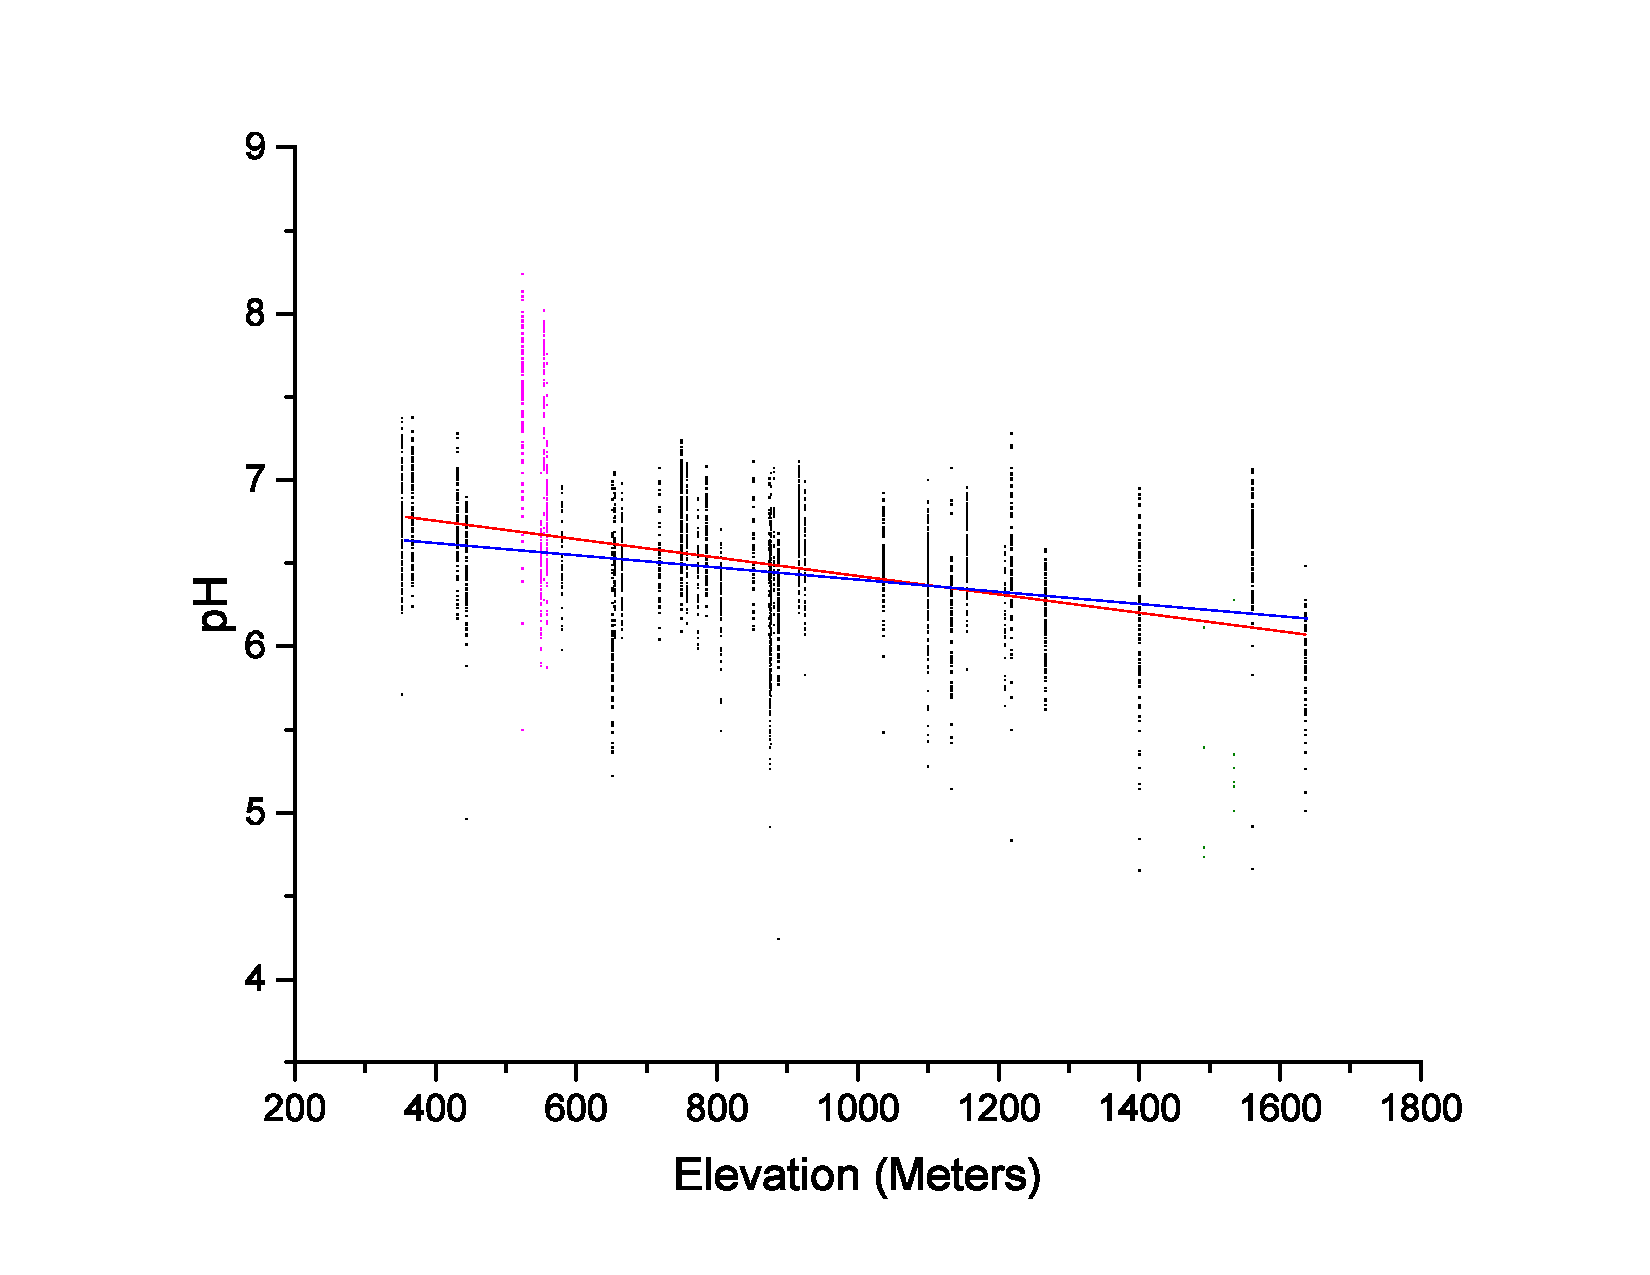
\includegraphics[width=6in]{pHdata}\\
  \caption{pH plotted vs. Elevation.  With and without outliers.}\label{fig:pHdata}
\end{figure}
\begin{verbatim}
Acid rain is believed to negatively affect The Great Smokey Mountain National Park.
Acid Deposition, more commonly known as Acid Rain, is a constant problem for the industrialized world. The amount of pollutants released into the atmosphere has risen since the industrial revolution.  The processes that industrial plants utilize excess sulfur oxides (SOx) and nitrogen oxides (NOx) into the atmosphere. This effluent production of chemicals creates problems for the world's environmental systems including acid deposition and other effects that can harm our health, our surface waters, our soils, and our structures.
Acid Deposition occurs when the emissions of sulfur oxides (SOx), and nitrogen oxides (NOx) react within the atmosphere and then the constituents and their newly created chemicals are deposited on the earth’s surface.  Acid Deposition has similar characteristics of regular precipitation but it has lower average pH of less than 4.5.  These pollutants can come down to ground in three ways: wet deposition (rain and snow), dry deposition (gases and particles), and fog or cloud deposition (occult).  Once the acid deposition constituents have entered in the environment they react with the surface waters, in the soil, and on man-made structures (Calvert, 1983).  This begins to acidify the surface waters which can harm any life forms that interact with it, it can acidify the soils and harm the plants, and it can degrade buildings.
Acid deposition greatly impacts surface water and the surrounding environment. The added pollutants affects the alkalinity of water, or its ability to buffer a change in acidity,  and results in a pH change.  As the pH level lowers, the ability of surface waters to sustain aquatic life also decline, this is called acidification. And while many factors affect the ability for the survival of aquatic life, acidification can be directly related to a lot of species survival.  
Acidification of bodies of water can be either chronic or episodic. Chronic acidification occurs when the body of water has constant low acid neutralizing capability (ANC); which creates a large area of  nearly un-inhabitable water where aquatic life would struggle to survive. Episodic acidification describes a rapid increase of acidity. Drastic acidification episodes result in large surges of nitrates and/or sulfates in surface waters. Episodes often occur during snow melts or heavy rains and are detrimental to aquatic life during the vulnerable early phases of life. (http://www.epa.gov/acidrain/effects/surface_water.html).
The Great Smoky Mountains National Park (GRSM) is located in the southern Appalachians straddling eastern Tennessee and western North Carolina.  While the second largest National Park in the eastern United States, comprising more than 220,000 hectares, it is the most-visited National Park with approximately 10 million visitors, twice the number of visitors to any other National Park, each year(Moore, 2001).  Furthermore GRSM is the largest undisturbed deciduous or coniferous forest-dominated area in the eastern United States (Delcourt and Delcourt, 1991).  The park is home to about 100 species of native trees, with the majority of the park is forest and nearly a quarter of that is old growth.  There are over 1,500 flowering plant species located in the GRSM along with 200 species of birds, 66 types of mammals, 50 native fish species, 39 kinds of reptiles, and 43 species of amphibians,  not to mention insects.  In recognition of the park's unique natural resources, the United Nations has designated GRSM as an International Biosphere Reserve, which are established to show a balance between people and nature (http://www.nps.gov/grsm/naturescience/index.htm). GRSM streams support a great number of fish species, amphibians, and benthic invertebrates; five streams in the GRSM have been designated as an Outstanding National Resource Waters (Neff, 2009).  The National Park Service (NPS) wishes to conserve the biodiversity of the park.Acid deposition negatively affects the 3,000 km of streams present in the GRSM and that impacts every living thing in the park which rely on the water quality in the park.  A literature review in (Neff 2007) approximates a pH of 6 for biological effects and a pH of 5 for mortality in trout for the park.  Exact threshold values are difficult to find because of the large number of influential factors such as species, age, egg versus fry versus adult, background water quality, exposure duration, etc.  While pH levels from 5 to 6 can be toxic in the presence of aluminum and can be harmful to eggs and fry in very soft waters in the lower end of the range.(Robinson 08).  
In order to monitor acid deposition the park has a program called the Inventory and Monitoring program.  An aspect of this program is a high elevation site, Noland Divide Watershed.  NDW is a small, 17.4 ha, watershed about 2 km east of Clingmans Dome, which is the second highest peak in the eastern US.  NDW contains sites to measure wet and dry deposition as well as "grab" samples to study in the lab.  This site is a continuation of the Integrated Forest Study (IFS) and was taken over by the park in 1991.  The IFS observed and quantified atmospheric deposition and nutrient cycling in forested watersheds.  The study demonstrated the upper elevations of the GRSM receive some of the highest loading rates of acidifying nitrogen and sulphur species in North America (Johnson and Lindberg, 1992).   The park wide Stream Survey is also part of the IFS and focuses on the park as a whole, this water quality monitoring network uses stream survey samples collected throughout the year in order to quantify water quality in the park.  Currently, samples are collected from 32 sites every two months and an additional 11 samples are collected twice per year.  These samples cover streams from 6 GRSM stream systems.  Every sample collected including NDW is processed in the lab for conductivity, pH, ANC, Chloride, Nitrate, Sulfate, Phosphate, Ammonium, Sodium, Potassium, Magnesium, Calcium, Aluminum, Copper, Iron, Manganese, Silicon, and Zinc.  Information leading to a bettering understanding of water quality conditions per watershed characteristics aids GRSM resource staff in managing the Park’s natural resources.  Other than chemistry the acidity of the park streams can be affected by geographical attributes such as geology and elevation. Stream acidification is more pronounced in higher elevation watersheds with underlying base-poor geology (Herligy et al. 1991, Hyer et al. 1995; Wigington et al. 1996a,b).  The acidification patterns along an elevational gradient occur throughout the Appalachian region similar to the data collected in the GRSM streams.  

Figure 1-1 
This figure shows all pH data from 1993 to 2012 vs. Elevation (m).  The red trend line includes abrams,  sites 237 and 252.  These outliers are removed for the blue trend line.

Figure 1 is a graph of all measured pH values for Stream Survey between the years of 1993 and 2012 graphed against the elevations they were collected.  Two notable figures are here, one that contains all pH data from 1993 to 2012 and another that has removed the outliers Abrams stream system along with sites 252 and 237.  The steeper sloped line represents the data set that still contains Abrams, sites 237, and 252.  This graph clearly illustrates pH trending downwards as elevation increases.  Increases in sulfate or nitrate in runoff and streams through acid deposition can cause an increase leaching of base cations, hydrogen ion, aluminum, and decreased ANC (Sullivan, 2004).  Leached aluminum can end up in streams and is toxic to fish (Driscoll 2003).  Rainfall and fog in the GRSM affect elevations above 4000 feet first higher elevations have steeper slopes which correlate to both thinner soils and base poor geology.  All these factors contribute to lower pH in higher elevations.  Neff et al. (2013) observed this trend, but found other basin factors correlate to chronic and episodic acidification.  Other basins factors include drainage area size, vegetation, and soil properties, which factors all are change within an elevational gradient.  
In support of GRSM natural resource management, stream water quality has been monitored since 1993, and this long-term dataset was recently statistically analyzed and commonly referred to as the “Biotic Effects Report” (Cai et al. 2013).  In this report, elevation was found to be a dominant driver for predicting water quality among the park’s stream.  Overall, results in this report found that stream pH and ANC decreased at -.32 units and -35.73 μeq L-1 respectively, per 1,000-ft elevation gain.  Conductivity, chloride, and base cations were also found to significantly decrease with elevation gain.  Sulfate showed no significant trend with elevation, however nitrate was found to significantly increase with elevation gain.  The GRSM 2011 Annual Water Quality Report compared pH trend lines representing the current 43 sites from 1993-2010 with 2011.  The data showed lines of similar slopes with different intercepts, which was interpreted to mean increasing pH at all elevations in GRSM streams.  Acid deposition increases with elevation in the GRSM and the higher elevation streams would experience increased sulfate, and prolonged acidification if soil desorption becomes a dominant geochemical watershed process which could occur if pH increased to 6.0 and sulfate dropped below 50 μeq L-1.  From a management perspective, the Biotic Effects Report contains limitations in the analyses to assess long-term changes because locations sampled have changed over time and most current sample locations are at lower elevations.

Table 1 shows the current historical elevation classes with the number of sites they include and the percent of sites in each band.  Although there were limitations, the biotic effects report provided essential information on how to improve future water quality and biological monitoring programs.
The National Park Service is currently developing a Vital Sign Monitoring Program for a number of national parks around the country, which includes the GRSM (Annual Administrative Report For Inventories and Vital Signs Monitoring FY 2010).  The goal of the GRSM Vital Sign Monitoring Program is to assess long-term changes in ecosystem health, including both terrestrial and aquatic environments. In addition, the program will integrate these environments and and include existing data on basin factors associated with water quality.   Although it is widely recognized that elevational gradient is important, a question about what elevation ranges are changing versus those that are not needs to be quantified in order to design an effective sampling program.  In addition, data must be collected at a set frequency to provide sufficient statistical power to make valid interpretations of change over time. 

Objectives of this study were to:
\begin{itemize}
\item  characterize time trends in stream pH and acidic anions among elevation ranges in order to assess whether conditions are improving or degrading, and 
\item characterize sampling variance based on available water quality data, within the context of time and elevation, to support development of the GRSM’s Vital Signs Monitoring Program.  In addition to supporting this Program, a cost analysis of selected water quality sampling schemes will be summarized.  The format of this thesis will follow these two objectives.  
\end{itemize}
\begin{itemize}
\item Has stream pH and acid anion concentrations changed among three time periods (1993-2002, 2003-2008, and 2009-2012), and among six elevation ranges (1000-2000ft, 2000-2500ft, 2500-3000ft, 3000-3500ft,3500-4500ft, 4500<)?
\begin{itemize}
 \item ANOVA
\item Time trends
\end{itemize}
\item What is the statistical power for water quality parameters based on frequency and elevational location based on historic data?
\begin{itemize}
\item Post Hoc Analysis
\item A Priori Analysis
\end{itemize}
\end{itemize}
The thesis is organized into two separate chapters following the two above research questions. Each chapter will follow the technical format of introduction, methods, results, and discussion.  
\end{verbatim}
    \chapter{Trend Analysis}\label{ch:TA}
\section{Methods}
\subsection{Introduction}
\begin{itemize}
	\item Trend analysis for Stream Survey has been done before and reported in \citep{robinson2008ph} and the Biotics effects report \citep{cai2012}
	\item A trend analysis of the data collected through the Stream Survey can be used to help determine the water quality of the streams
	\item The most important trend is the trend for pH
	\item {\bf Outline} The trend analysis will be conducted on Stream Survey data spanning the years 1993-2012 using the statistical program JMP 
	for determining outliers and the statistical program SPSS for the actual trend analysis.
\end{itemize}
\subsection{Body}
\begin{itemize}
    \item A trend analysis will answer the continuing question concerning the overall health of the park which is, "How are the streams doing?".  
    More specifically "Is the pH trending towards a higher pH or a lower pH?"
    \subsubsection{Data}
    \begin{itemize}
        \item The data comes from years of analyzing water samples collected through the Stream Survey and is tabulated into a running data set.
        \item A single trend line could be made to encompass all 20 years worth of water quality data, but this would make discovering the cause of the trends
        more difficult.
        \item Assuming ecosystems try to achieve equilibrium the change observed over all time should be zero.
        \item So in order to easier learn from this trend analysis, it will be logically broken up into smaller sets of years.
        \item Different sets may have different positive or negative trends for which separate hypothesis have been or can be formulated and tested in this trend
        analysis.
        \item The separate data sets are between time and between elevation classes.  There were three different time sets created.  The first time set covers the years 1993 to 2002, these are the same years analyzed in \citep{robinson2008ph}.  The remaining years were broken up at 2008, which was the year that the Kingston and Bull run power plants installed scrubbers onto their stacks.  So with the six different elevation classes and the three different time sets there are eighteen different data sets that are analyzed in this paper. 
\begin{table}[htbp]
\caption{These elevation classes were created to add more weight to the higher elevations}
\begin{tabular}{clcp{5cm}}
\toprule
Elevation Classes & Meters (Feet)                              & n & Site \# \\ 
\midrule
1                        & 304.8-609.6 (1000-2000)           & 5   & 13 ,23, 24, 30, 479 \\ 
2                        & 609.6-762 (2000-2500)              & 9   & 4, 311, 268, 480, 310, 483, 147, 148, 484 \\ 
3                        & 762-914.4 (2500-3000)              & 13 & 114, 481, 482, 149, 66, 492, 137, 293, 270, 493, 485, 144, 224 \\ 
4                        & 914.4-1066.8 (3000-3500)         & 4   & 143, 142, 73, 71 \\ 
5                        & 1066.8-1371.6 (3500-4500)       & 4   & 74, 221, 251, 233 \\ 
6                        & $1371.6< (4500<)$                    & 2   & 253, 234 \\ 
\bottomrule
\end{tabular}
\label{tab:ElevationBands}
\end{table}
\end{itemize}
    \end{itemize}
    \subsubsection{Instruments}
    \begin{itemize}
    	\item done usisng statistical programs.
        \item Outliler determination and trend hypothesis.
        \begin{itemize}
        	\item Plot pH on y-axis vs. all time.  This visually represents that the slope does not equal zero.  Check outliers in this plot.  If they can be explained then fix or delete them. 
        	\item Plot pH on y-axis vs. elevation.  Visually check for trend of decreasing pH as elevation increases.
        	\item Plot pH vs. month.  To check for seasonality.
        	\item Outliers found include Abrams, Anakeesta sites, and storm flow.  Abrams is consistently found as an out lier within GRSM water quality projects using stream survey data for statistical purposes.  Abrams is located in the Cades Cove area of the park and sits in natural limestone bedrock.  This limestone increases the ANC of the streams so much that many of  the measured Abrams pH values are high enough to be outliers and are thrown out of the data.
        	\item Water quality at sites 237 and 252 are heavily influenced by Anakeesta geology introduced into the streams through road cuts.
        	\item Storm flow is also usually seen as an out lier in past GRSM water quality projects.  Storms can bring high intensity rain fall which can very quickly raise the levels of nitrate and sulfate pollution in the streams.  The runoff can also carry any pollutants that have come to rest on vegetation or the ground.  The lowered pH of the streams caused by the storm flow can cause leeching of the surrounding mineral geology in affected areas. Healthy streams can rebound to normal pH values, unhealthy streams can have lowered ANC due to the leaching.  Measurements taken from storm flow can show uncharacteristically low pH values and high amounts of metals.  In this way storm flow is sometimes considered an out lier.  Much of the water quality data has been characterized as base flow and storm flow by Dr.Cai, but not all it.  Water quality data after 2010 has not been characterized.  Dismissing all of  storm flow as an out lier is complicated by this lack of information.  Either; storm flow and base flow would need to be determined for the 2011 and 2012 data,all of the 2011 and 2012 data could be left out, or 2011 and 2012 would need to be characterized as base flow or storm flow.  Throwing out the years 2011 and 2012 would leave the last time set with only two years of data.  The data was compared with and without storm flow observations.  It was determined to manually select out lier storm flow observations.  They can be removed on a case by case basis during the regression procedure.
	\item review output  for normality, heteroscedasticity, cook's D, DFBETAS, DFFITS.
	\item Find proposed out lier in original data
	\item Justify its removal, remove it and run the regression method again
	\item The outputs will change every time an observation is removed.
	\end{itemize}
	\begin{table}[htbp]
\caption{Equations created through step-wise variable selection}
\begin{tabular}{lp{7.5cm}cc}
\toprule
Dependent (n)     &Model                                                                                                                                                                                                                                                                                                                                                                                                       & Adjusted $r^2$  & Model p \\ 
\midrule
pH (3116)            &$.673\times\log_2(\text{Sum Base Cations}) + (-.368\times \text{NO}_3) + (.262\times \text{Julian Day}) + (-.266\times \text{SO}_4) + (-.050\times\cos(\theta))$                                                                                                                                       & 0.630                  & $<$0.001 \\
ANC (3116)         &$ (.415\times \text{Sum Base Cations}) + (-.185\times \text{SO}_4) + (.595\times \text{Conductivity}) + (-.102\times \text{NO}_3) + (.019\times \text{Julian Date}) + (.005\times \text{Cl}) + (.005\times \sin(\theta))$                                                & 0.984                  & 0.049 \\
NO$_3$ (3116)   &$(-.295\times \text{SO}_4) + (-3.183\times \text{ANC}) + (2.19\times \text{Conductivity}) + ( .923\times \text{Sum Base Cations}) + (.120\times \text{Julian Date}) + (.051\times \text{Cl}) + (.047\times \sin(\theta)) + (.031\times \cos(\theta))$ &0.498                   & 0.017 \\ 
SO$_4$ (3116)   &$ (-.166\times \text{NO}_3) + (2.318\times \text{Conductivity}) + (-3.229\times \text{ANC}) + (1.033\times \text{Sum Base Cations}) + (.042\times \text{Julian Date})$                                                                                                                               & 0.720                  & $<$0.001 \\ 
\bottomrule
\end{tabular}
\label{tab:stepwiseeq}
\end{table}

	\item The variable selected through this process were used to create fixed models to be used while discovering the Julian Date coefficient for each water quality variable in each data set.
	\item If the step-wise equation had at least one time variable in it(Julian date, $\sin(\theta), \cos(\theta)$) then the rest were added.  This is presented in \autoref{variables}.
	\item along with the step-wise regression method, another regression analysis was done using only time based variables.  These are the Julian Date, $\sin(\theta)$, and $\cos(\theta)$ time variables.  This method was used to find trends in the water quality variables that are related to time only.		
        \item IBM's SPSS was used to conduct this trend analysis.
        \item These options were chosen for regression and assumptions for this procedure include.(from notebook and textbook)
\end{itemize}

\section{Results}
\begin{itemize}
	\item In \citep{robinson2008ph} table 4 reports julian date coefficients for four water quality variables (pH, ANC, NO$_3$, SO$_4$) by each elevation band.
	\begin{itemize}
		\item A similar layout was used in \autoref{tab:Step-wise julian date} and \autoref{tab:time vars}.
		\item This was done for continuity and ease of comparison.
	\end{itemize}
	\item The first trend analysis was completed using the step-wise method for choosing predictors and the results are presented in \autoref{tab:Step-wise julian date}
	\item The second trend analysis uses only time based variables as predictors and these results are presented in \autoref{tab:time vars}
	\item Both tables are modeled after table 4 in \citep{robinson2008ph}
	\item Each table is further divided into three different time sets: 1993-2002, 2003-2008, 2009-2012.
	\item Each of these time sets are further divided into six elevation bands
	\item Each of elevation band has the results of four trend lines, one for each of the studied water quality variables (pH, ANC, NO$_3$, SO$_4$).
	\item Each trend line is represented by its Julian date coefficient, the r$^2$ value for the trend line, and it's statistical significance.
	\item 2 of the 72 trend lines in \autoref{tab:Step-wise julian date} are insignificant.  In contrast only 20 of the trend lines in \autoref{tab:time vars} are significant.
	\item Insignificance is determined  by receiving a p-value greater than .05, the $\alpha$ of the trend line.  A p-value greater than .05 rejects the hypothesis that $\beta$ $\neq$ 0.  There is greater than a 5$\%$ chance that $\beta$=0.  There is to much chance of no trend line for the scientific community.
	\item Repeat trends from previous thesis
	\item Compare to \citep{robinson2008ph}, his trends are negative.
\end{itemize}
\section{Discussion}
\begin{itemize}
	\item Why were the trends insignificant?
	\item Why are the water quality trends trending the way they are at separate time sets ( discuss comparisons between sets in the ANOVA bonferoni section).
	\item How should the water quality variables have behaved based on known properties and \citep{robinson2008ph}.
	\item Very generally speaking these results are different than \citep{robinson2008ph} predicted.
	\item Water quality will continue to get better.
	\begin{itemize}
		\item because pollution is being regulated
	\end{itemize}
	\item there are still unknowns and prediction is still hard.
\end{itemize}
	
    \chapter{Means Comparison}\label{ch:mc}

\section{Methods}

\subsection{Introduction}
Bull run and Kingston power plants installed scrubbers on their smokestacks in the year 2008 in order to decrease sulfate and nitrate emissions.
These scrubbers have significantly reduced the amount of sulfur dioxide emitted by the smoke stacks.
According to \autoref{fig:sulfateemissions}, which is a bar chart depicting the sum of sulfur dioxide emissions of Kingston and Bull run power plants,  the sulfur dioxide concentration dropped from 80 thousand tons in 2008 to about 15 thousand tons in 2009.

Noland divide is a high elevation site located just below Clingman's Dome, which is the highest point in the Great Smokey Mountains.  
It has been studied for acid deposition since the late 80's and contains three separate sample collection sites.
The through fall site collects deposition that has had a chance to fall through the trees and thus collects extra pollutants resting there.
There is also an open to air site which is designed to collect deposition that has not run through the trees and then grab samples are collected from two nearby streams.
Samples from Noland Divide are continuously collected and analyzed every two weeks with the same lab processes as the Stream Survey samples.

Interestingly the through fall SO$_4$ concentrations dramatically decline from about 115 $\mu$eq L$^{-1}$ in 2007 to about 30 $\mu$eq L$^{-1}$ in 2010.
\begin{figure}[h!]
  \centering
  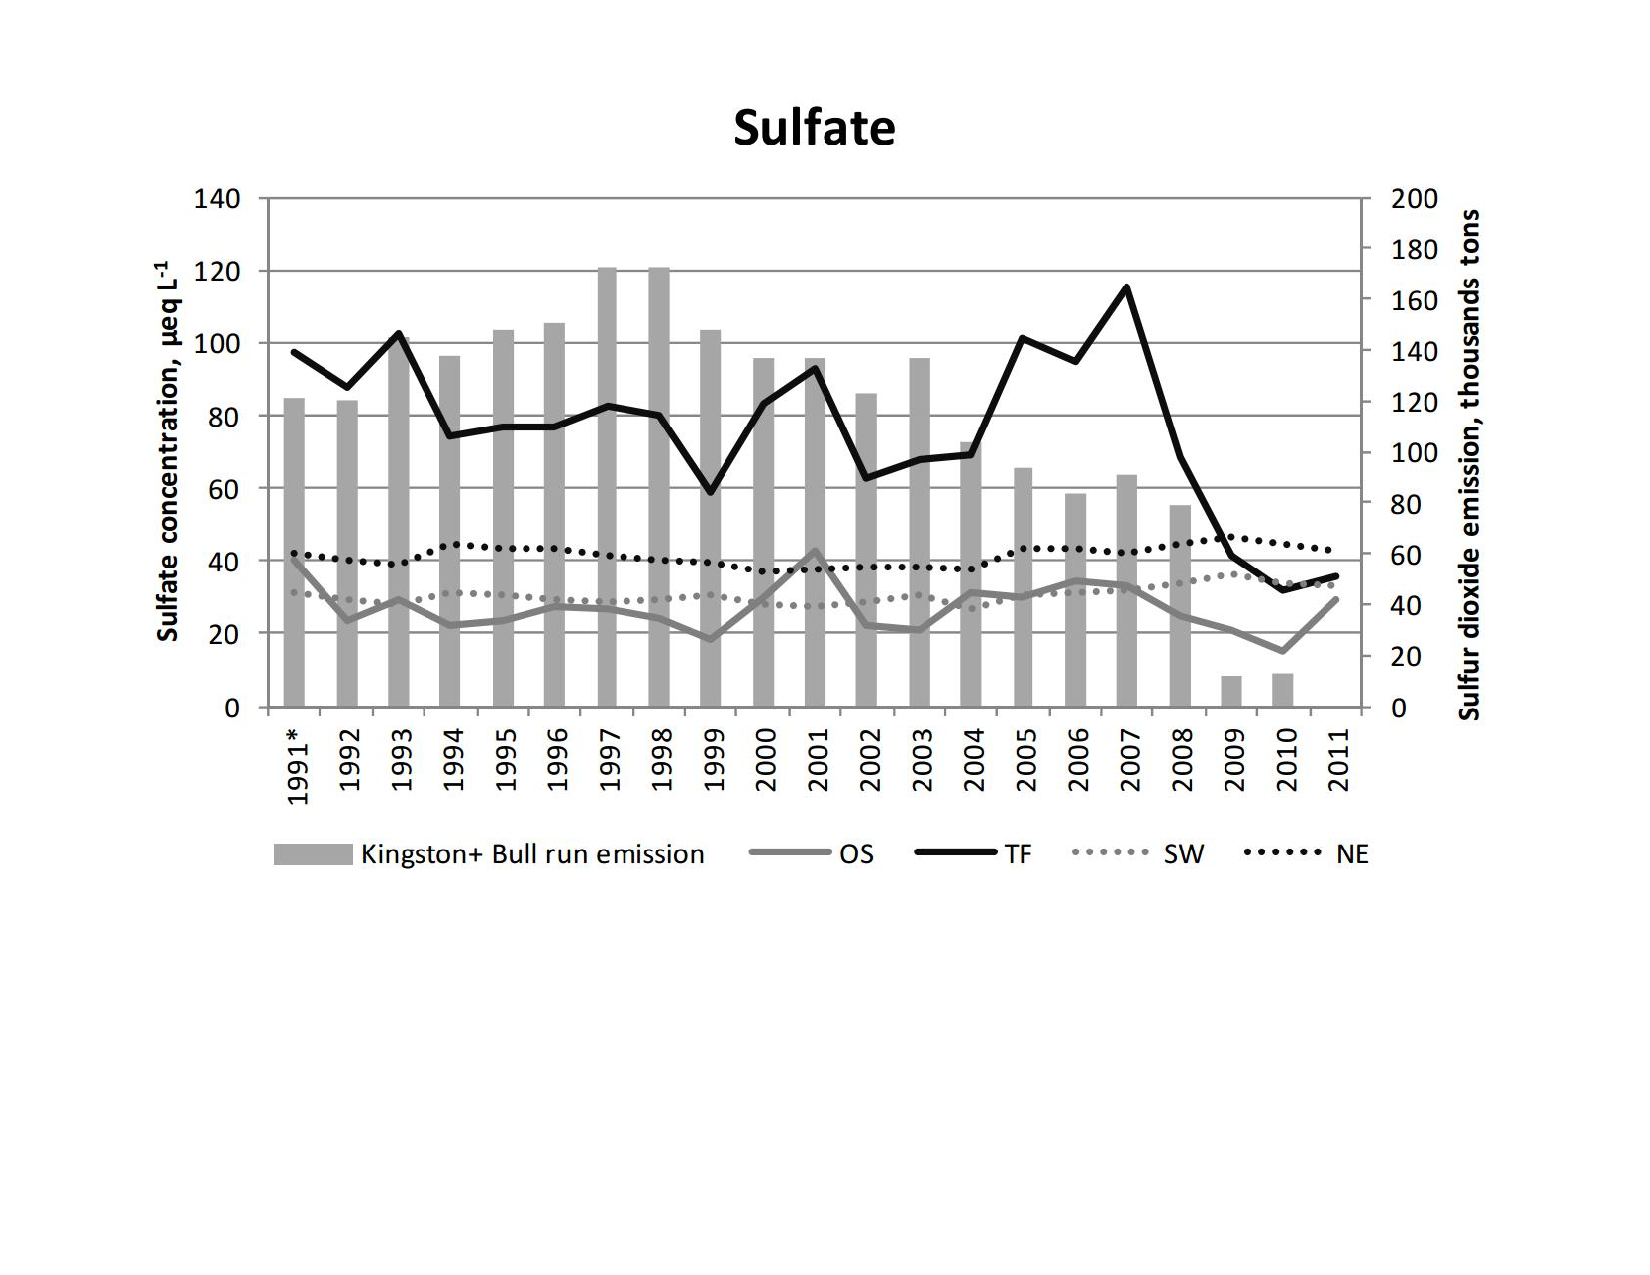
\includegraphics[width=6in]{SulfateEmissions}\\
  \caption{Sulfate emmisions of Kingstion and Bull run against those measured in Noland high elevation site \citep{annualreport2012}.}\label{fig:sulfateemissions}
\end{figure}
A decrease in sulfur dioxide emissions could correlate to the decrease in SO$_4$ concentrations measured in Noland Divide through fall.
The effects of air pollution will be more pronounced and easier to recognize at a high elevation site such as Noland Divide but one site cannot represent the whole park.
The geographical spread and number of sites contained within the Stream Survey can give a fuller representation of the affects of air pollution from local power plants.
And assuming that the sulfur dioxide emissions from Kingston and Bull run power plants affect the whole GRSM park then there may be signals for this affect in the data.
To explorer for these signals each water quality vector in each time set will be tested against each other by way of means comparison methods.
A significant difference between the data before and after the scrubbers were installed would indicate reason for further study.

\subsubsection{Instruments}
ANOVA is a common means comparison method, but it is not best when testing more than one hypothesis at once.
As more hypothesis are added the chances of finding a rare occurrence rises, which is the chance to reject the null hypothesis (the means being equal) when it is actually true (type I error).
The proposed analysis requires testing for the equality of three separate time sets and thus three separate hypothesis at once.
The Bonferroni adjustment solves this by dividing the alpha by the number of hypothesis being tested.
In this way multiple hypothesis are tested as if there is only one.

Two outputs are created by the Bonferroni method: one graphical and one numerical.
The graphical output presents a line graph showing the means of each group analyzed.
An observer can use this output to see the actual group means along with a visual representation of their differences.
The numerical output presents a table of pairwise listings of all the groups compared to each other.
Each pair listed is evaluated by their 95$\%$ confidence intervals and the significance associated with each comparison.
If the confidence interval includes zero then the groups are statistically the same or equal.

Using SPSS and the Bonferroni method three time sets (93-02, 03-08, 09-12) will be compared at six elevation class levels and across four water quality variables (pH, ANC, NO$_3$, and SO$_4 $).
Each group compared is the same data groups from the stream survey data analyzed in \autoref{ch:TA} and \autoref{ch:poweranslysis}.

\section{Results}

\begin{table}[htbp]
\caption{Bonferroni comparisons between multiple groups}
\begin{center}
\begin{tabular}{p{2cm}cccccccccccc}
\toprule
 Elevation Classes& \multicolumn{ 3}{c}{pH} & \multicolumn{ 3}{c}{ANC} & \multicolumn{ 3}{c}{Nitrate} & \multicolumn{ 3}{c}{Sulfate} \\ \cline{2-13}\noalign{\smallskip}
 & \multicolumn{ 1}{c}{1-2} & 1-3 & 2-3 & 1-2 & 1-3 & 2-3 & 1-2 & 1-3 & 2-3 & 1-2 & 1-3 & 2-3 \\  \cline{2-13}
\multicolumn{1}{c}{1} & \textbf{$\neq$} & \textbf{$\neq$} & \textbf{$\neq$} & \textbf{=} & \textbf{=} & \textbf{=} & \textbf{$\neq$} & \textbf{=} & \textbf{=} & \textbf{=} & \textbf{=} & \textbf{=} \\ 
\multicolumn{1}{c}{2} & \textbf{=} & \textbf{=} & \textbf{=} & \textbf{=} & \textbf{$\neq$} & \textbf{=} & \textbf{$\neq$} & \textbf{$\neq$} & \textbf{=} & \textbf{$\neq$} & \textbf{$\neq$} & \textbf{=} \\ 
\multicolumn{1}{c}{3} & \textbf{$\neq$} & \textbf{$\neq$} & \textbf{$\neq$} & \textbf{=} & \textbf{$\neq$} & \textbf{=} & \textbf{=} & \textbf{$\neq$} & \textbf{$\neq$} & \textbf{=} & \textbf{=} & \textbf{=} \\ 
\multicolumn{1}{c}{4} & \textbf{=} & \textbf{$\neq$} & \textbf{$\neq$} & \textbf{=} & \textbf{=} & \textbf{=} & \textbf{=} & \textbf{=} & \textbf{=} & \textbf{=} & \textbf{=} & \textbf{=} \\ 
\multicolumn{1}{c}{5} & \textbf{$\neq$} & \textbf{$\neq$} & \textbf{$\neq$} & \textbf{=} & \textbf{$\neq$} & \textbf{$\neq$} & \textbf{$\neq$} & \textbf{=} & \textbf{$\neq$} & \textbf{=} & \textbf{=} & \textbf{=} \\ 
\multicolumn{1}{c}{6} & \textbf{=} & \textbf{$\neq$} & \textbf{$\neq$} & \textbf{=} & \textbf{=} & \textbf{=} & \textbf{=} & \textbf{=} & \textbf{=} & \textbf{=} & \textbf{=} & \textbf{=} \\ 
\bottomrule
\end{tabular}
\end{center}
\label{tab:Bontable}
\end{table}
The group means comparisons are represented by equal signs and unequal signs and are taken from the 95$\%$ C.I. determined in the analysis.
In \autoref{tab:Bontable} there are three columns per water quality variable and each column represents the comparison of two groups of the same variable in different times.
All groups that were found to be equal were insignificant and all groups that were unequal are significant at the familywise 0.05 $\alpha$ level.

The line graphs can be helpful in comparing the sizes of mean differences between the three time sets.
These figures are not as definitive as the results in \autoref{tab:Bontable} because a noticeable visual difference does not always correspond to a significant difference, but they can still be useful as visual tools.
There are six figures for each of the water quality variables, one for each of the elevation classes.
They are presented in \autoref{app:bon}.

%For the most part the figures representing pH seem to be continuing a similar rate of change through the years, but this is also misleading because the time sets do not contain equal numbers of years.

The set comparisons for pH are the first comparisons presented, they contain more unequal sets than any other water quality variable.
Much of the comparisons are unequal except between elevation class 2 which are all equal and class 4 and 6 which show are equal in sets 1 and 2.
If a pronounced elevational trend existed for pH in the GRSM, this trend would be visible in the Bonferroni line graphs.
Following the means of each time set through the different elevation classes the largest mean should be in elevation class 1 and the smallest in elevation class 6.
Unfortunately elevation class 2 always contains the lowest means instead of Elevation class 6.
And elevation class 3 behaves as if it should be between elevation class 5 and 6.

In contrast to the pH line graphs, the ANC line graphs do not all have similar rates of change.
In the odd numbered classes ANC reached a peak in set 2 and dropped for set 3.
All of the ANC figures have a decreasing trend from set 2 to 3 except for class 2 which is steadily increasing. 
The set means presented in the ANC figures vary greatly in concentration.
Classes and 1 and 2 are more than double the means of the other classes.
The ANC concentrations of elevation class 2 are the lowest which helps explain why the pH of elevation class 2 is also the lowest.
It is important to note here that even though class 2's concentrations are the lowest, they are also the only concentrations that are increasing.
The analysis found more equality than inequality in ANC, and in fact all three time sets in elevation classes 1, 4, and 6 were are all found to be equal.  
Only 4 set comparisons were found to be unequal: comparisons between time sets 1 and 3 at elevation classes 2, 3, and 5, and the comparison between time sets 2 and 3 at elevation class 5.

NO$_3$ elevation classes 4 and 6 are equal across all time sets and elevation class 3 shows time sets 1 and 2 being equal while 3 is not.  
Elevation class 1 is the opposite of expected, which is all time sets being unequal with time set 3, showing all being equal except for sets 1 and 2.  
In elevation class 2 sets 3 and 2 are equal and in elevation class 5 sets 3 and 1 are equal.
The line graphs for the odd numbered elevation classes of NO$_3$ all have decreasing mean values from set 2 to 3.
In elevation classes 2 and 4 the mean values for set 3 are higher than those in set 2 but the difference of the means over times is decreasing.
Overall the NO$_3$ figures show mostly decreasing concentrations over time, except for class 6 which is always increasing.
And the odd classes all have decreasing negative trends from set 2 to set 3 while classes 2 and 4 have decreasing positive trends between set 2 and 3.

SO$_4$ points to all three time sets being equal across all elevation classes except for class 2, which shows equality for time sets 2 and 3.  
The line graphs can sometimes be misleading when visually comparing the time set mens and it is always best to have the confidence intervals on hand.
For example when looking at the SO$_4$ figures many of the means look different across the time sets, but according to the table, except for class 2, they are all equal across time sets.
All of the set 3 means for SO$_4$ are larger than their respective set 2 means except for those in class 2 which has negative trends throughout.

\section{Discussion}
This analysis was completed in expectation of patterns similar to time sets 1 and 2 having significantly different means from time set 3.
This expectation was based on the installation of scrubbers on the Kingston and Bull-run power plants and \autoref{fig:sulfateemissions}.
Overall these patterns were not noticed, the clearest evidence is the complete equality down the column of time sets 2 and 3 for SO$_4$.
Other outcomes were also unexpected such as the increase in pH over time and the abnormal ANC concentrations.
The apparent decrease in ANC overtime as indicated in the Bonferroni figures was unexpected both because this is in contrast to the Julian date coefficients for ANC and pH has an increasing trend overtime.
Because the Bonferroni method calculates significant means for the water quality vector the difference between the figures and the trends suggests error in the trend analysis models.

The focus of this chapter was to investigate the decline in sulfur dioxide emissions from the Kingston and Bull run power plants and how it may have impacted the decline in SO$_4$  concentrations in the through fall measurements of the Noland divide high elevation site.
If a correlation existed it would be apparent in the pH results, but especially in the SO$_4$ results.
A significant negative difference in means for set 3 compared to sets 1 and 2 would support the hypothesis.
The inequalities present between the sets of pH data display a possible connection to the decline in sulfur dioxide pollution but there are many other factors that effect stream pH.
The comparisons between the SO$_4$ sets are unfortunately mostly equal.
This suggests a bank of SO$_4$ where previous SO$_4$ pollution is collected and a steady concentration is being released into the steams which are being measured with grab samples.
In this way until that bank is depleted a significant difference in means may not be found.
%sulfate sequestration?

    \chapter{Power Analysis} \label{ch:poweranslysis}
\section{Methods}
\subsection{Introduction}
\begin{itemize}
	\item Statistics come with an inherent amount of error.
	\item The trend lines created in the trend analysis chapter have a defined error called type II error or $\beta$.
	%add a small table of error types
	\item $\beta$ describes failure to reject a false null hypothesis or failure to detect a trend in the data when there really is one.
	\item $\beta$ is usually described in terms of probability and it's opposite is called power(1-$\beta$)
	\item The power of a statistical test describes the probability that the test is true.
	\item The statistical test is the hypothesis test which tests if the coefficients of a regression line are zero.  So whether or not a trend exists.
	\item The power of the trend lines will state the "truth" of the slope of the trend.  A trend lilne with a power of 1.00 means that there is a 100$\%$ chance that the calculated slope is not zero.
	\item Using the earlier calculated trend lives as input, the power of each regression line was calculated with the help of G*power.  An a priori analysis was calculated to help determine the number of samples needed for desired levels of power.
\end{itemize}
\subsection{Body}
\begin{itemize}
	\item The objectives of the power analysis are to determine the power of the trend lines calculated from past observations and to determine an adaquate number of samples needed for different levels of power for the future.
	\item The inputs needed in the G*power program for a post hoc analysis are: number of observations (N), adjusted r$^2$, number of predictors, and Effect size.  N and adj.r$^2$ are  outputs from the trend analysis and effect size is calculated using G*power.  These values are reported in \autoref{tab:SWposthoc} and \autoref{tab:TVposthoc}.
	\item A post hoc analysis of the trend line data from \autoref{tab:TVposthoc} is not useful.  This is because most of the lines have terribly low r$^2$ values and are insignificant trend lines.  The power of an insignificant trend line is also insignificant.
	\item Post hoc analysis and a priori were  run on both methods for trend lines
	\item G*power is a free power analysis program written by four germen psychology professors.
	\item It runs the gamut in power analysis options and uses methods stated in \citep{cohen1992power}.
	\item G*power was used to calculate powers in the post hoc analysis and sample sizes for the a priori analysis.
	\item Excel was used along with results provided by G*power to create scenarios to finish up the a priori analysis.
\end{itemize}
\subsection{Procedures}
\subsubsection{Post hoc}
\begin{itemize}
	\item Data compiled in \autoref{tab:SWposthoc} and \autoref{tab:TVposthoc} give the inputs required for a post hoc power analysis on th previously created trend lines.
	\item required inputs for G*power include, ES(Effect Size), $\alpha$(alpha), number of observations, and number of predictors.
	\begin{itemize}
		\item ES is calculated in G*power by the Cohen method stated in \citep{cohen1992power} "A Power Primer".
		\item Alpha refers to the $\alpha$ of the trend lines (.05).
		\item Number of observations is given in trend line output from SPSS.
		\item Number of predictors is also stated in trend line output.
	\end{itemize}
	\item The calculate button will calculate the power
	\begin{itemize}
		\item This is all that is needed for a post hoc analysis.  It answers the question "What was the power of the survey ?" or "How strong are the trend lines that were computed?"
	\end{itemize}
	\item The calculated powers are reported along side their trend line inputs in \autoref{tab:SWposthoc} and \autoref{tab:TVposthoc}.
\end{itemize}
\subsubsection{A priori}
\begin{itemize}
	\item The a priori analysis can help survey planners to create a sampling survey that will produce trend lines with certain ES values and powers.
	\item There are two objectives to this analysis which are to create "power graphs", which are plots of power vs. sample size.  The other is to plan out an actual scenario for which samples can be added or subtracted to elevation bands for a desired power of .80 and an ES of .15.
	\item The power graphs are created in G*power using the "x-y plot for a range of values" button next to the "calculate" button.
	\item They-axis has the power values while the x-axis contains the number of observations or samples.  The power will increase with number of samples until it reaches 100.
	\item Four power graphs were created, one for each water quality variable.  If ES and power are set to .15 and .80 respectively for every presumed trend line then the only variable is number of predictors.  The number of predictors is set for each water quality variable (pH, ANC, NO$_3$,SO$_4$).  Taken from the earlier step-wise selection method (link to step-wise table).  Therefore only one "power graph" is needed for every trend line in each variable.
	\item ES and power can be chosen or kept constant based on reports by Cohen.
	\item Cohen's standardizations
	\item While the "power graphs" are useful in planning for the future of the stream survey, it can be shown that if ES and power are chosen, exact numbers of samples and sites can be added and subtracted from elevation bands.
	\begin{table}[htbp]
		\caption{A priori calculation in G*power when alpha, ES, and power are set to .05, .15, and .80 respectively.}
		\begin{center}
		\begin{tabular}{lcc}
		\hline\noalign{\smallskip}
		 & \multicolumn{1}{l}{Number of predictors} & N \\  \hline\noalign{\smallskip}
		pH & 6 & 98 \\ 
		ANC & 8 & 109 \\ 
		Nitrate & 8 & 109 \\ 
		Sulfate & 7 & 103 \\ 
		Time & 3 & 77 \\  \hline
		\end{tabular}
		\end{center}
		\label{APN}
		\end{table}%needs to be cleaned up
	\item The rest was done in excel
	\item This calculated number of observations can be divided by the number of samples collected in one year to get the number of years required to reach a power of .80.
	\item The analysis can be further conducted by calculating the number of samples per year to achieve a power of .80.  For this calculation all water quality variables were given the highest number of samples of 110 and 77 was used for the trends using only time variables.
		\begin{table}[htbp]
\caption{samples/year to achieve a power .80}
\begin{center}
\begin{tabular}{lrrrr}
\hline\noalign{\smallskip}
Years & 1 & 2 & 3 & 4 \\ \cline{2-5}\noalign{\smallskip}
Water Quality Variables & 110 & 55 & 37 & 28 \\ 
Time Variables & 77 & 39  & 26  & 19  \\ \hline\noalign{\smallskip}
\end{tabular}
\end{center}
\label{sytaapeighty}
\end{table}%needs to be cleaned up
	\item \autoref{sytaapeighty} is needed to calculate number of samples needed per elevation band to achieve a power of .80.  This number of samples can then be further divided to get a number of sites needed to achieve a power of .80.  If a trend line with a power of .80 is desired after one year ,for all water quality variables to be satisfied, 110 samples need to be collected.  If four years are waited then only 28 samples need to be collected per year.
	\item  To create this final table the number of samples per elevation  band was subtracted from the number of samples to achieve a power of .80 which gives us the number of samples needed in addition to what is currently collected to receive a power of .80.  These results are organized into samples needed per elevation band to achieve a power of .80 and seperated by years depending of how many years of data go into the trend lines.

\end{itemize}
\section{Results}
\subsection{Post hoc}
\begin{itemize}
	\item A post hoc power analysis was conducted for each of the two methods of trend analysis.
	\item \autoref{tab:SWposthoc} and \autoref{tab:TVposthoc} record the results of the post hoc analysis on the trend lines with variables created through the step-wise method and the trend lines created using only time variables respectively.  Included in these tables are the number of samples and r$^2$ variables from the trend analysis and effect size and power from the post hoc analysis.
	\item \autoref{tab:SWposthoc} and \autoref{tab:TVposthoc} are broken into the four analyzed water quality variables (pH, ANC, NO$_3$,SO$_4$) and divided into the tree time sets (93-02, 03-08, 09-12), and then further divided into the six elevation classes.
	\item use results from previous draft
	\item any similar power analysis?
\end{itemize}
\subsection{A priori}
\subsubsection{Power graphs}
\begin{itemize}
	\item The results of the a priori power analysis will be the most important for planning.
	\item The usual output is the "power graph" which plots power on the y-axis and total sample size on the x-axis.
	\item G*power outputs some very nice power graphs. The power graphs created from the a priori power analysis are presented in \autoref{fig:pHPowerGraph}, \autoref{fig:ANCnNPowerGraph}, \autoref{fig:SulfatePowerGraph}, and \autoref{fig:TVPowerGraph}.
	\item There were four power graphs created, three for the water quality variables and one for the time variables.  ANC and Nitrate both have the same number of predictors from the step-wise variable selection method and therefore create the same power graph. 
	\item each graph contains 3 lines representing 3 different ES choices: .15, .25, and .35.  These were chosen to mimic the choices of small, medium, and large effects standardized by Cohen in \citep{cohen1992power}.  Limitations of the G*power program left the best choices to be .15, .25, and .35.   A small effect of .02 was ignored because preliminary graph results showed it to be  not useful.	
\end{itemize}
\subsubsection{Planning with power analysis}
\begin{itemize}
	\item Using the ability of the a priori power analysis to compute a number of samples needed for a certain power, a scenario was played out to see how many sites needed to be added or could be removed from an elevation band in the stream survey.
	\begin{table}[htbp]
\caption{Years to acheive a power of .80}
\begin{tabular}{clccccc}
\toprule
\multicolumn{1}{p{2cm}}{Elevation Bands} & \multicolumn{1}{c}{Site \#} & \multicolumn{1}{p{2cm}}{Current n/yr} & pH &\multicolumn{1}{p{1cm}}{ ANC NO$_3$} & SO$_4$ & \multicolumn{1}{p{3cm}}{Time variables} \\  
\midrule
1 & 13 ,23, 24, 30, 479 & 26 & 3.77  & 4.19  & 3.96  & 2.96  \\ 
2 & \multicolumn{1}{p{4cm}}{4, 311, 268, 480, 310, 483, 147, 148, 484} & 34 & 2.88  & 3.21  & 3.03  & 2.26  \\ 
3 & \multicolumn{ 1}{p{4cm}}{114, 481, 482, 149, 66, 492, 137, 293, 270, 493, 485, 144, 224} & \multicolumn{ 1}{c}{62} & \multicolumn{ 1}{c}{1.58 } & \multicolumn{ 1}{c}{1.76 } & \multicolumn{ 1}{c}{1.66 } & \multicolumn{ 1}{c}{1.24} \\ 
4 & 143, 142, 73, 71 & 24 & 4.08  & 4.54  & 4.29  & 3.21  \\ 
5 & 74, 221, 251, 233 & 22 & 4.45  & 4.95  & 4.68  & 3.50  \\ 
6 & 253, 234 & 12 & 8.17  & 9.08  & 8.58  & 6.42  \\  
\bottomrule
\end{tabular}
\label{tab:currentyrsto.80}
\end{table}%needs to be cleaned
	\item This scenario was followed through with both methods of trend lines.
	\item \autoref{currentyrsto.80} records the six elevation bands along with the site numbers that belong to them.  In the column labeled ,current n per year, the amount of samples collected per elevation band in the year 2012 was tabulated.  The values in the remaining columns were calculated by dividing the number of samples given in \autoref{APN} by the current samples per year column in \autoref{currentyrsto.80}.
	\item Looking at the table there are 26  samples collected in elevation band one in one year.  In order to compute a trend line that receives a power of .80 with pH as the dependent  samples would need to be collected for 3.77 years before the trend line is computed.   The larges is elevation class for a trend line in ANC or NO$_3$ which requires 9.08 years.
	\begin{table}[htbp]
\caption{Necesary sites scenario for water quality variables}
\begin{tabular}{ccccc|ccccc}
\cline{2-9}
\multicolumn{1}{c}{} &   \multicolumn{4}{c}{ \#Samples required} & \multicolumn{4}{c}{\# sites required} \\ \cline{2-9}\noalign{\smallskip}
\multicolumn{1}{p{3cm}}{Elevation Bands}  & 1 yr  & 2 yrs   & 3 yrs    & 4 yrs   & 1 yr   & 2 yrs  & 3 yrs  & 4 yrs\\ \hline\noalign{\smallskip}
1 &  84 & 29 & 11   & 2    & 14 & 5  & 2   & 0 \\ 
2  & 76 & 21 & 3     & -7   & 13 & 4  & 0   & -1 \\ 
3 &  48 & -7  & -25 & -35 & 8   & -1 & -4 & -6 \\
4 &  86 & 31 & 13  & 4     & 14 & 5  & 2  & 1 \\ 
5 &  88 & 33 & 15  & 6     & 15 & 6  & 2  & 1 \\ 
6 &  98 & 43 & 25  & 16   & 16 & 7  & 4  & 3 \\ \hline
\end{tabular}
\label{tab:WQapsenario}
\end{table}%needs to be cleaned
	\begin{table}[htbp]
\centering
\caption{Necessary sites scenario for time variables}
\begin{tabular}{ccccc|ccccc}
\toprule
\multicolumn{1}{c}{} &  \multicolumn{4}{c}{ \#Samples required} & \multicolumn{4}{c}{\# sites required} \\ \cline{2-9}\noalign{\smallskip}
\multicolumn{1}{p{3cm}}{Elevation Bands}  & 1 yr   & 2 yrs  & 3 yrs     & 4 yrs   & 1 yr  & 2 yrs & 3 yrs  & 4 yrs \\ \midrule
1 &  51 & 13 & 0 & -7 & 9 & 2 & 0 & -1 \\ 
2 &  43 & 5 & -8 & -15 & 7 & 1 & -1 & -2 \\ 
3 &  15 & -24 & -36 & -43 & 3 & -4 & -6 & -7 \\ 
4 &  53 & 15 & 2 & -5 & 9 & 2 & 0 & -1 \\ 
5 &  55 & 17 & 4 & -3 & 9 & 3 & 1 & 0 \\ 
6 &  65 & 27 & 14 & 7 & 11 & 4 & 2 & 1 \\ \bottomrule
\end{tabular}
\label{tab:TVapsenario}
\end{table}
	\item The left side of both \autoref{WQapsenario} and \autoref{TVapsenario} show how many more samples are required to get a trend line with a power of .80. 
	\item  In \autoref{WQapsenario} for elevation class 3, 48 more samples need to be collected if a trend line with a power of .80 is to be created after one year.  But if a trend line can wait to be created after two years, then there is a surplus of seven samples per year.  If four years can be waited there is a surplus of 35 samples which on the right side of the table translates into a surplus of 6 whole site locations per year.
	\item \autoref{TVapsenario} works the same way as \autoref{WQapsenario} but of course it uses different variables for the trend lines.
	\item results from previous draft
	\item any other papers like this?
\end{itemize}
\section{Discussion}
\subsection{Post hoc}
\begin{itemize}
	\item The results presented in \autoref{tab:SWposthoc} and \autoref{tab:TVposthoc} show how the calculated power is highly affected by number of observations more than anything else.
	\item In \autoref{tab:SWposthoc}, even when the r$^2$ and ES values are relatively low if the N is greater than 100 then the power is excellent.
	\item \autoref{tab:TVposthoc} show the effect of the ES on power.  Other than these lines being insignificant, many of the ES values are small according to Cohen and when compared to \autoref{tab:SWposthoc}.  Low ES values and low observations create low powers.  Low ES values com from low r$^2$ values.  The low r$^2$ values can be blamed for the insignificance of the lines and the poor powers. 
	\item Some lines are just not well described by Julian Date,$\sin$($\theta$), and $\cos$($\theta$) only.
\end{itemize}
\subsection{A priori}
\begin{itemize}
	\item How can these results be used?
	\item How can these results be manipulated?	
	\item The results in \autoref{tab:WQapsenario} and \autoref{tab:TVapsenario} can help with both of the problems of The park wanting a cheaper survey and researchers wanting more high elevation sites.
	
	\item The table can be used to re-organize sites across bands.
	\begin{itemize}
		\item In the current SS scheme there is a surplus of sites in lower elevation bands and a deficit for sites in higher elevations.
		\item Looking at the right side of \autoref{tab:WQapsenario}, if trends are desired after four years of data with a power of .80 and an ES of .15, seven sites may be taken from elevation bands 2 and 3 and 5 would need to be added to elevation bands 4,5, and 6.
		\item After this re-arrangement two sites may be completely discontinued.
		\item This saves time, effort, and money, but it is a very specific scenario.		
	\end{itemize}
	\item The downside of an a priori power analysis is that once you pick all the variables that go into it, you can' t change them in the future
	\begin{itemize}
		\item Variables that can change include how you divide the sites into elevation bands
		\item Trend line creation (alpha, variable selection)
		\item Power analysis ( power, and ES)
	\end{itemize}
	\item If during the hypothetical situation in which four years are waited to do another trend analysis, a better model is found, then the survey would need to be re-evaluated to reflect the new model.
	\begin{itemize}
		\item the model could require a different number of sites
	\end{itemize}
	\item Choices for power and ES could change
	\item planning with the a priori power analysis requires guessing the trends for the future.  % Thesis Conclusion?
	\item This guess will probably be based on the past , such as this one.
	\item This guess assumes that trends of the past will continue into the future
	\item The ANOVA/Bonferoni and the comparison between \citep{robinson2008ph} and the current trends shows that this is difficult.
	\item better understanding is needed
	\item At the end of the day the trends are positive!
\end{itemize}
	
    %%%%%%%%%%%%%%%%%%%%%%%%%%%%%%%%%%%%%%%%%%%%%%%%%%%%%%%%%%%%%%%%%%%%%%%%%%%%%%%%%%%%%%%%%%%%%%%%%%%%%
    % BIBLIOGRAPHY
    %%%%%%%%%%%%%%%%%%%%%%%%%%%%%%%%%%%%%%%%%%%%%%%%%%%%%%%%%%%%%%%%%%%%%%%%%%%%%%%%%%%%%%%%%%%%%%%%%%%%%
    \makeBibliographyPage % make the bibliography title page - can be edited in ut-thesis-template.tex
    \bibliographystyle{apalike} % bibliography style - recommend using apalike-doi as it hyperlinks DOIs
    \bibliography{references/references-dissertation} % references.bib included in the references directory
    %%%%%%%%%%%%%%%%%%%%%%%%%%%%%%%%%%%%%%%%%%%%%%%%%%%%%%%%%%%%%%%%%%%%%%%%%%%%%%%%%%%%%%%%%%%%%%%%%%%%%
    % APPENDIX - OPTIONAL - COMMENT IF NOT NEEDED
    %%%%%%%%%%%%%%%%%%%%%%%%%%%%%%%%%%%%%%%%%%%%%%%%%%%%%%%%%%%%%%%%%%%%%%%%%%%%%%%%%%%%%%%%%%%%%%%%%%%%%
    \makeAppendixPage   % make the appendix title page - can be edited in ut-thesis-template.tex
    \appendix
    %try to get all of the titles on the same page as the table or graph
\chapter{Site Data}\pagebreak

	\section{Site Data}
		\begin{table}[h]\scriptsize
\centering
\caption{GRSM Stream Survey site descriptions}
\begin{tabular}{ccll}
\toprule
      & Site ID & Site Description                                                   &Watershed\\ 
\midrule
1   & 173       & Mill Creek above Abrams Creek                             & Abrams\\
2   & 174       & Abrams Creek below Cades Cove                         & Abrams \\ 
3   & 488       & Mill Creek at Pumphouse on Forge Creek Road     & Abrams \\ 
4   & 489       & Abrams Creek 300 m below trailhead bridge         & Abrams \\ 
5   & 142       & Beech Creek above Lost Bottom Creek                 & Cataloochee \\ 
6   & 143       & Lost Bottom Creek (Cataloochee Creek)               & Cataloochee \\ 
7   & 144       & Palmer Creek above Pretty Hollow Creek              & Cataloochee \\ 
8   & 147       & Lower Cataloochee Creek                                      & Cataloochee \\ 
9   & 148       & Lower Little Cataloochee Creek                             & Cataloochee \\ 
10 & 149       & Middle Cataloochee Creek at bridge                      & Cataloochee \\ 
11 & 293       & Rough Fork at Caldwell House                               & Cataloochee \\ 
12 & 493       & Palmer Creek at Davidson Branch Trail                  & Cataloochee \\ 
13 & 4           & Lower Rock Creek                                                  & Cosby \\ 
14 & 114       & Cosby Creek at log bridge                                     & Cosby \\ 
15 & 137       & Upper Rock Creek (Cosby Creek)                          & Cosby \\ 
16 & 492       & Camel Hump Creek off Low Gap Trail                     & Cosby \\ 
17 & 221       & Hazel Creek above cascades                                 & Hazel \\ 
18 & 224       & Hazel Creek just below Proctor Creek Confluence & Hazel \\ 
19 & 310       & Bone Valley Creek (Hazel Creek)                            & Hazel \\ 
20 & 311       & Hazel Creek below Haw Gap Creek                        & Hazel \\ 
21 & 479       & Hazel Creek at Campsite 86                                   & Hazel \\ 
22 & 480       & Haw Gap Creek at bridge near Campsite 84          & Hazel \\ 
23 & 481       & Little Fork above Sugar Fork Trail                           & Hazel \\ 
24 & 482       & Sugar Fork above Little Fork                                  & Hazel \\  
25 & 483       & Sugar Fork above Haw Gap Creek                         & Hazel \\ 
26 & 484       & Hazel Creek at Cold Spring Gap Trail                      & Hazel \\ 
27 & 485       & Walker Creek above Hazel Creek Trail                   & Hazel \\ 
28 & 13         & Little River at boundary                                         & Little \\ 
29 & 23         & Lower Middle Prong Little River                              & Little \\ 
30 & 24         & Lower West Prong Little River                                & Little \\ 
31 & 30         & West Prong Little Pigeon at Headquarters             & Little\\ 
32 & 66         & West Prong Little Pigeon at Chimneys Picnic Area & Little \\ 
33 & 71         & Road Prong above barrier cascade                        & Little \\ 
34 & 73         & Walker Camp Prong above Road Prong                 & Little \\ 
35 & 74         & Walker Camp Prong above Alum Cave Creek        & Little \\ 
36 & 233       & Walker Camp Prong above Alum Cave                  & Little \\ 
37 & 234       & Upper Road Prong                                                 & Little \\ 
38 & 237       & Walker Camp Prong at last bridge                         & Little \\ 
39 & 251       & Beech Flats above US 441 loop                             & Oconaluftee \\ 
40 & 252       & Beech Flats below roadcut                                    & Oconaluftee \\ 
41 & 253       & Beech Flats above roadcut                                   & Oconaluftee \\ 
42 & 268       & Oconaluftee River below Smokemont                   & Oconaluftee \\ 
43 & 270       & Beech Flats at Kephart Footbridge                       & Oconaluftee \\  
\bottomrule
\end{tabular}
\label{tab:Site Data}
\end{table}\pagebreak

		\begin{table}[p]\scriptsize
\centering
\caption{GRSM site data continued}
\begin{tabular}{ccccccccc}
\toprule
    & \multicolumn{ 1}{p{1cm}}{Site ID} & \multicolumn{ 1}{p{1.4cm}}{Elevation (ft)} & \multicolumn{ 1}{p{1.4cm}}{Elevation (m)} & slope & Latitude   & Longitude  & \multicolumn{ 1}{p{2cm}}{Historical Elevation Classes} & \multicolumn{ 1}{p{1.4cm}}{New elevation classes} \\  
\midrule
1   & 173                                                 & 1715                                                          & 522.73                                                       & 35.68 & 35.59104 & -83.85361 & 3                                                                                      & 3 \\ 
2   & 174                                                 & 1715                                                          & 522.73                                                       & 10.27 & 35.59186 & -83.85308 & 3                                                                                      & 3 \\ 
3   & 488                                                 & 1790                                                          & 545.59                                                       & 4.04   & 35.58349 & -83.83446 & 4                                                                                      & 1 \\ 
4   & 489                                                 & 1710                                                          & 521.21                                                       & 32.78 & 35.59145 & -83.85397 & 4                                                                                      & 1 \\ 
5   & 142                                                 & 3300                                                          & 1005.84                                                     & 32.42 & 35.63565 & -83.14537 & 5                                                                                      & 2 \\ 
6   & 143                                                 & 3280                                                          & 999.74                                                       & 35.69 & 35.63625 & -83.14481 & 6                                                                                      & 2 \\ 
7   & 144                                                 & 2990                                                          & 911.35                                                       & 35.66 & 35.63900 & -83.13078 & 5                                                                                      & 2 \\ 
8   & 147                                                 & 2460                                                          & 749.81                                                       & 16.84 & 35.66688 & -83.07277 & 4                                                                                      & 3 \\ 
9   & 148                                                 & 2475                                                          & 754.38                                                       & 7.58   & 35.66913 & -83.07283 & 4                                                                                      & 3 \\ 
10 & 149                                                 & 2550                                                          & 777.24                                                       & 4.45   & 35.64627 & -83.07554 & 5                                                                                      & 3 \\ 
11 & 293                                                 & 2755                                                          & 839.72                                                       & 18.73 & 35.62442 & -83.11391 & 5                                                                                      & 4 \\ 
12 & 493                                                 & 2840                                                          & 865.63                                                       & 33.10 & 35.63462 & -83.11943 & 6                                                                                      & 6 \\ 
13 & 4                                                     & 2080                                                          & 633.98                                                       & 6.11   & 35.76133 & -83.21044 & 3                                                                                      & 1 \\ 
14 & 114                                                 & 2510                                                          & 765.05                                                       & 13.71 & 35.74863 & -83.20066 & 5                                                                                      & 2 \\ 
15 & 137                                                 & 2750                                                          & 838.20                                                       & 22.92 & 35.74616 & -83.21630 & 5                                                                                      & 2 \\ 
16 & 492                                                 & 2730                                                          & 832.10                                                       & 25.86 & 35.74457 & -83.19876 & 5                                                                                      & 6 \\ 
17 & 221                                                 & 4000                                                          & 1219.20                                                     & 30.02 & 35.54632 & -83.58283 & 8                                                                                      & 3 \\ 
18 & 224                                                 & 2999                                                          & 914.00                                                       & 17.92 & 35.53212 & -83.62234 & 6                                                                                      & 3 \\ 
19 & 310                                                 & 2240                                                          & 682.75                                                       & 19.63 & 35.49994 & -83.68014 & 4                                                                                      & 4 \\ 
20 & 311                                                 & 2155                                                          & 656.84                                                       & 26.20 & 35.49377 & -83.68852 & 4                                                                                      & 5 \\ 
21 & 479                                                 & 1740                                                          & 530.35                                                       & 39.70 & 35.47233 & -83.71933 & 3                                                                                      & 5 \\ 
22 & 480                                                 & 2201                                                          & 671.00                                                       & 10.07 & 35.49474 & -83.68873 & 4                                                                                      & 5 \\ 
23 & 481                                                 & 2540                                                          & 774.19                                                       & 30.90 & 35.50256 & -83.70835 & 5                                                                                      & 5 \\ 
24 & 482                                                 & 2540                                                          & 774.19                                                       & 38.66 & 35.50236 & -83.70859 & 5                                                                                      & 6 \\ 
25 & 483                                                 & 2320                                                          & 707.14                                                       & 34.29 & 35.49947 & -83.69494 & 4                                                                                      & 6 \\ 
26 & 484                                                 & 2475                                                          & 754.38                                                       & 9.11   & 35.50331 & -83.65930 & 5                                                                                      & 1 \\ 
27 & 485                                                 & 2860                                                          & 871.73                                                       & 5.17   & 35.52249 & -83.63101 & 6                                                                                      & 1 \\ 
28 & 13                                                   & 1100                                                          & 335.28                                                       & 44.21 & 35.66763 & -83.71450 & 2                                                                                      & 1 \\ 
29 & 23                                                   & 1150                                                          & 350.52                                                       & 5.96   & 35.65724 & -83.70979 & 2                                                                                      & 1 \\ 
30 & 24                                                   & 1150                                                          & 350.52                                                       & 31.60 & 35.65682 & -83.71017 & 2                                                                                      & 1 \\ 
31 & 30                                                   & 1430                                                          & 435.86                                                       & 2.17   & 35.68819 & -83.53672 & 2                                                                                      & 1 \\ 
32 & 66                                                   & 2680                                                          & 816.86                                                       & 17.92 & 35.63723 & -83.49484 & 5                                                                                      & 2 \\ 
33 & 71                                                   & 3400                                                          & 1036.32                                                     & 31.28 & 35.63440 & -83.47032 & 6                                                                                      & 2 \\ 
34 & 73                                                   & 3360                                                          & 1024.13                                                     & 28.98 & 35.63476 & -83.46931 & 6                                                                                      & 2 \\ 
35 & 74                                                   & 3820                                                          & 1164.34                                                     & 18.07 & 35.62912 & -83.45102 & 7                                                                                      & 2 \\ 
36 & 233                                                 & 4255                                                          & 1296.92                                                     & 21.86 & 35.61830 & -83.42718 & 8                                                                                      & 3 \\ 
37 & 234                                                 & 5000                                                          & 1524.00                                                     & 23.93 & 35.60975 & -83.45043 & 10                                                                                    & 3 \\ 
38 & 237                                                 & 4520                                                          & 1377.70                                                     & 30.21 & 35.62409 & -83.41692 & 9                                                                                      & 3 \\ 
39 & 251                                                 & 4010                                                          & 1222.25                                                     & 19.03 & 35.60226 & -83.41533 & 8                                                                                      & 3 \\ 
40 & 252                                                 & 4680                                                          & 1426.46                                                     & 33.32 & 35.60666 & -83.43391 & 9                                                                                      & 3 \\ 
41 & 253                                                 & 4760                                                          & 1450.85                                                     & 26.42 & 35.60682 & -83.43510 & 9                                                                                      & 3 \\ 
42 & 268                                                 & 2169                                                          & 661.00                                                       & 3.31   & 35.55293 & -83.30937 & 4                                                                                      & 4 \\ 
43 & 270                                                 & 2799                                                          & 853.00                                                       & 22.92 & 35.58641 & -83.36400 & 5                                                                                      & 4 \\  
\bottomrule
\end{tabular}
\label{tab:Site Data}
\end{table}\pagebreak


\chapter{Descriptive Statistics}\label{sec:DescriptiveStats}\pagebreak
	
	\section{pH}
		% Table generated by Excel2LaTeX from sheet 'Descriptive Stats'
\begin{table}[htbp]
  \centering
	\caption{pH Descriptive Statistics}
    \begin{tabular}{rrlcccc}
    \toprule
    Set                                                                                                                                     & Class                           & Elevation m (ft)                                                 & N     & Minimum & Maximum & Mean \\
    \midrule
    \multicolumn{1}{c}{\multirow{6}[2]{*}{\begin{sideways}1993-2002\end{sideways}}} & \multicolumn{1}{c}{1} & \multicolumn{1}{l}{304.8-609.6 (1000-2000)} & 327   & 4.96  & 7.90  & 6.57  \\
    \multicolumn{1}{c}{}                                                                                                         & \multicolumn{1}{c}{2} & \multicolumn{1}{l}{609.6-762 (2000-2500)}    & 393   & 5.32  & 7.00  & 6.25  \\
    \multicolumn{1}{c}{}                                                                                                         & \multicolumn{1}{c}{3} & \multicolumn{1}{l}{762-914.4 (2500-3000)} & 400   & 4.65  & 8.24  & 6.44  \\
    \multicolumn{1}{c}{}                                                                                                         & \multicolumn{1}{c}{4} & \multicolumn{1}{l}{914.4-1066.8 (3000-3500)} & 121   & 6.18  & 7.11  & 6.50  \\
    \multicolumn{1}{c}{}                                                                                                         & \multicolumn{1}{c}{5} & \multicolumn{1}{l}{1066.8-1371.6 (3500-4500)} & 116   & 6.07  & 7.05  & 6.50  \\
    \multicolumn{1}{c}{}                                                                                                         & \multicolumn{1}{c}{6} & \multicolumn{1}{l}{1371.6$<$ (4500$<$)} & 110   & 5.77  & 7.06  & 6.41  \\
\midrule
    \multicolumn{1}{c}{\multirow{6}[2]{*}{\begin{sideways}2003-2008\end{sideways}}} & \multicolumn{1}{c}{1} & \multicolumn{1}{l}{304.8-609.6 (1000-2000)} & 255   & 5.22  & 7.95  & 6.65  \\
    \multicolumn{1}{c}{}                                                                                                         & \multicolumn{1}{c}{2} & \multicolumn{1}{l}{609.6-762 (2000-2500)} & 289   & 4.83  & 7.07  & 6.32  \\
    \multicolumn{1}{c}{} & \multicolumn{1}{c}{3} & \multicolumn{1}{l}{762-914.4 (2500-3000)} & 299   & 4.65  & 8.10  & 6.55  \\
    \multicolumn{1}{c}{} & \multicolumn{1}{c}{4} & \multicolumn{1}{l}{914.4-1066.8 (3000-3500)} & 119   & 5.95  & 7.06  & 6.58  \\
    \multicolumn{1}{c}{} & \multicolumn{1}{c}{5} & \multicolumn{1}{l}{1066.8-1371.6 (3500-4500)} & 35    & 5.98  & 7.03  & 6.50  \\
    \multicolumn{1}{c}{} & \multicolumn{1}{c}{6} & \multicolumn{1}{l}{1371.6$<$ (4500$<$)} & 97    & 5.79  & 7.05  & 6.44  \\
\midrule
    \multicolumn{1}{c}{\multirow{6}[2]{*}{\begin{sideways}2009-2012\end{sideways}}} & \multicolumn{1}{c}{1} & \multicolumn{1}{l}{304.8-609.6 (1000-2000)} & 191   & 5.42  & 8.02  & 6.77  \\
    \multicolumn{1}{c}{} & \multicolumn{1}{c}{2} & \multicolumn{1}{l}{609.6-762 (2000-2500)} & 212   & 4.91  & 7.28  & 6.47  \\
    \multicolumn{1}{c}{} & \multicolumn{1}{c}{3} & \multicolumn{1}{l}{762-914.4 (2500-3000)} & 228   & 4.73  & 7.96  & 6.68  \\
    \multicolumn{1}{c}{} & \multicolumn{1}{c}{4} & \multicolumn{1}{l}{914.4-1066.8 (3000-3500)} & 97    & 6.20  & 7.08  & 6.68  \\
    \multicolumn{1}{c}{} & \multicolumn{1}{c}{5} & \multicolumn{1}{l}{1066.8-1371.6 (3500-4500)} & 29    & 6.30  & 7.11  & 6.77  \\
    \multicolumn{1}{c}{} & \multicolumn{1}{c}{6} & \multicolumn{1}{l}{1371.6$<$ (4500$<$)} & 76    & 4.24  & 7.09  & 6.52  \\
    \bottomrule
    \end{tabular}%
  \label{tab:DSpH}%
\end{table}%
\pagebreak

	\section{ANC}
		% Table generated by Excel2LaTeX from sheet 'Descriptive Stats'
\begin{table}[htbp]
  \centering
	\caption{ANC Descriptive Statistics}
    \begin{tabular}{rrlcccc}
    \toprule
    Set   & Class & Elevation m (ft) & N     & Minimum & Maximum & Mean \\
    \midrule
    \multicolumn{1}{c}{\multirow{6}[2]{*}{\begin{sideways}1993-2002\end{sideways}}} & \multicolumn{1}{c}{1} & \multicolumn{1}{l}{304.8-609.6 (1000-2000)} & 327   & -20.74  & 1534.47  & 149.76  \\
    \multicolumn{1}{c}{} & \multicolumn{1}{c}{2} & \multicolumn{1}{l}{609.6-762 (2000-2500)} & 392   & -7.43  & 182.95  & 40.75  \\
    \multicolumn{1}{c}{} & \multicolumn{1}{c}{3} & \multicolumn{1}{l}{762-914.4 (2500-3000)} & 398   & -19.97  & 1624.49  & 158.44  \\
    \multicolumn{1}{c}{} & \multicolumn{1}{c}{4} & \multicolumn{1}{l}{914.4-1066.8 (3000-3500)} & 120   & 24.45  & 178.00  & 75.84  \\
    \multicolumn{1}{c}{} & \multicolumn{1}{c}{5} & \multicolumn{1}{l}{1066.8-1371.6 (3500-4500)} & 116   & 41.34  & 162.76  & 77.06  \\
    \multicolumn{1}{c}{} & \multicolumn{1}{c}{6} & \multicolumn{1}{l}{1371.6$< (4500<$)} & 110   & 15.64  & 165.02  & 68.01  \\\midrule
    \multicolumn{1}{c}{\multirow{6}[2]{*}{\begin{sideways}2003-2008\end{sideways}}} & \multicolumn{1}{c}{1} & \multicolumn{1}{l}{304.8-609.6 (1000-2000)} & 255   & -37.09  & 1314.56  & 173.48  \\
    \multicolumn{1}{c}{} & \multicolumn{1}{c}{2} & \multicolumn{1}{l}{609.6-762 (2000-2500)} & 289   & -1.88  & 145.95  & 42.20  \\
    \multicolumn{1}{c}{} & \multicolumn{1}{c}{3} & \multicolumn{1}{l}{762-914.4 (2500-3000)} & 299   & -26.45  & 1591.06  & 172.82  \\
    \multicolumn{1}{c}{} & \multicolumn{1}{c}{4} & \multicolumn{1}{l}{914.4-1066.8 (3000-3500)} & 119   & 23.36  & 128.28  & 69.90  \\
    \multicolumn{1}{c}{} & \multicolumn{1}{c}{5} & \multicolumn{1}{l}{1066.8-1371.6 (3500-4500)} & 35    & 36.37  & 115.80  & 77.84  \\
    \multicolumn{1}{c}{} & \multicolumn{1}{c}{6} & \multicolumn{1}{l}{1371.6$< (4500<$)} & 97    & 6.73  & 130.63  & 55.68  \\\midrule
    \multicolumn{1}{c}{\multirow{6}[2]{*}{\begin{sideways}2009-2012\end{sideways}}} & \multicolumn{1}{c}{1} & \multicolumn{1}{l}{304.8-609.6 (1000-2000)} & 191   & -0.02  & 1377.93  & 164.72  \\
    \multicolumn{1}{c}{} & \multicolumn{1}{c}{2} & \multicolumn{1}{l}{609.6-762 (2000-2500)} & 212   & -11.74  & 174.52  & 44.45  \\
    \multicolumn{1}{c}{} & \multicolumn{1}{c}{3} & \multicolumn{1}{l}{762-914.4 (2500-3000)} & 228   & -18.28  & 1535.69  & 160.14  \\
    \multicolumn{1}{c}{} & \multicolumn{1}{c}{4} & \multicolumn{1}{l}{914.4-1066.8 (3000-3500)} & 97    & 25.70  & 107.58  & 64.13  \\
    \multicolumn{1}{c}{} & \multicolumn{1}{c}{5} & \multicolumn{1}{l}{1066.8-1371.6 (3500-4500)} & 29    & 40.10  & 115.94  & 73.55  \\
    \multicolumn{1}{c}{} & \multicolumn{1}{c}{6} & \multicolumn{1}{l}{1371.6$< (4500<$)} & 76    & -3.92  & 114.28  & 46.15  \\
    \bottomrule
    \end{tabular}%
  \label{tab:DSANC}%
\end{table}%
\pagebreak

	\section{Nitrate}
		% Table generated by Excel2LaTeX from sheet 'Descriptive Stats'
\begin{table}[htbp]
  \centering
	\caption{Nitrate Descriptive Statistics}
    \begin{tabular}{rrlcccc}
    \toprule
    Set   & Class & Elevation m (ft) & N     & Minimum & Maximum & Mean \\
    \midrule
    \multicolumn{1}{c}{\multirow{6}[2]{*}{\begin{sideways}1993-2002\end{sideways}}} & \multicolumn{1}{c}{1} & \multicolumn{1}{l}{304.8-609.6 (1000-2000)} & 275   & 0.00  & 49.94  & 12.04  \\
    \multicolumn{1}{c}{} & \multicolumn{1}{c}{2} & \multicolumn{1}{l}{609.6-762 (2000-2500)} & 377   & 1.37  & 73.76  & 26.62  \\
    \multicolumn{1}{c}{} & \multicolumn{1}{c}{3} & \multicolumn{1}{l}{762-914.4 (2500-3000)} & 365   & 0.00  & 96.13  & 26.14  \\
    \multicolumn{1}{c}{} & \multicolumn{1}{c}{4} & \multicolumn{1}{l}{914.4-1066.8 (3000-3500)} & 105   & 2.16  & 28.29  & 11.90  \\
    \multicolumn{1}{c}{} & \multicolumn{1}{c}{5} & \multicolumn{1}{l}{1066.8-1371.6 (3500-4500)} & 66    & 1.23  & 10.55  & 4.35  \\
    \multicolumn{1}{c}{} & \multicolumn{1}{c}{6} & \multicolumn{1}{l}{1371.6$< (4500<$)} & 81    & 1.56  & 60.46  & 21.13  \\\midrule
    \multicolumn{1}{c}{\multirow{6}[2]{*}{\begin{sideways}2003-2008\end{sideways}}} & \multicolumn{1}{c}{1} & \multicolumn{1}{l}{304.8-609.6 (1000-2000)} & 252   & 0.50  & 62.75  & 16.56  \\
    \multicolumn{1}{c}{} & \multicolumn{1}{c}{2} & \multicolumn{1}{l}{609.6-762 (2000-2500)} & 296   & 0.62  & 67.12  & 29.20  \\
    \multicolumn{1}{c}{} & \multicolumn{1}{c}{3} & \multicolumn{1}{l}{762-914.4 (2500-3000)} & 297   & 0.13  & 95.72  & 27.69  \\
    \multicolumn{1}{c}{} & \multicolumn{1}{c}{4} & \multicolumn{1}{l}{914.4-1066.8 (3000-3500)} & 121   & 1.87  & 55.67  & 17.51  \\
    \multicolumn{1}{c}{} & \multicolumn{1}{c}{5} & \multicolumn{1}{l}{1066.8-1371.6 (3500-4500)} & 30    & 1.45  & 26.48  & 7.59  \\
    \multicolumn{1}{c}{} & \multicolumn{1}{c}{6} & \multicolumn{1}{l}{1371.6$< (4500<$)} & 98    & 1.09  & 72.79  & 24.88  \\\midrule
    \multicolumn{1}{c}{\multirow{6}[2]{*}{\begin{sideways}2009-2012\end{sideways}}} & \multicolumn{1}{c}{1} & \multicolumn{1}{l}{304.8-609.6 (1000-2000)} & 191   & 0.22  & 62.14  & 16.31  \\
    \multicolumn{1}{c}{} & \multicolumn{1}{c}{2} & \multicolumn{1}{l}{609.6-762 (2000-2500)} & 212   & 4.43  & 72.17  & 30.08  \\
    \multicolumn{1}{c}{} & \multicolumn{1}{c}{3} & \multicolumn{1}{l}{762-914.4 (2500-3000)} & 228   & 1.04  & 72.16  & 26.23  \\
    \multicolumn{1}{c}{} & \multicolumn{1}{c}{4} & \multicolumn{1}{l}{914.4-1066.8 (3000-3500)} & 97    & 0.54  & 34.67  & 18.72  \\
    \multicolumn{1}{c}{} & \multicolumn{1}{c}{5} & \multicolumn{1}{l}{1066.8-1371.6 (3500-4500)} & 29    & 0.21  & 83.68  & 6.44  \\
    \multicolumn{1}{c}{} & \multicolumn{1}{c}{6} & \multicolumn{1}{l}{1371.6$< (4500<$)} & 76    & 0.16  & 79.04  & 32.17  \\
    \bottomrule
    \end{tabular}%
  \label{tab:DSNO3}%
\end{table}%
\pagebreak

	\section{Sulfate}
		% Table generated by Excel2LaTeX from sheet 'Descriptive Stats'
\begin{table}[htbp]
  \centering
	\caption{Sulfate Descriptive Statistics}
    \begin{tabular}{rrlcccc}
    \toprule
    Set   & Class & Elevation m (ft) & N     & Minimum & Maximum & Mean \\
    \midrule
    \multicolumn{1}{c}{\multirow{6}[2]{*}{\begin{sideways}1993-2002\end{sideways}}} & \multicolumn{1}{c}{1} & \multicolumn{1}{l}{304.8-609.6 (1000-2000)} & 325   & 12.32  & 85.01  & 36.09  \\
    \multicolumn{1}{c}{} & \multicolumn{1}{c}{2} & \multicolumn{1}{l}{609.6-762 (2000-2500)} & 390   & 0.00  & 159.51  & 51.68  \\
    \multicolumn{1}{c}{} & \multicolumn{1}{c}{3} & \multicolumn{1}{l}{762-914.4 (2500-3000)} & 391   & 0.00  & 262.37  & 54.00  \\
    \multicolumn{1}{c}{} & \multicolumn{1}{c}{4} & \multicolumn{1}{l}{914.4-1066.8 (3000-3500)} & 119   & 12.34  & 77.74  & 25.16  \\
    \multicolumn{1}{c}{} & \multicolumn{1}{c}{5} & \multicolumn{1}{l}{1066.8-1371.6 (3500-4500)} & 116   & 7.51  & 79.98  & 26.14  \\
    \multicolumn{1}{c}{} & \multicolumn{1}{c}{6} & \multicolumn{1}{l}{1371.6$< (4500<$)} & 110   & 14.71  & 61.16  & 28.35  \\\midrule
    \multicolumn{1}{c}{\multirow{6}[2]{*}{\begin{sideways}2003-2008\end{sideways}}} & \multicolumn{1}{c}{1} & \multicolumn{1}{l}{304.8-609.6 (1000-2000)} & 261   & 10.00  & 93.23  & 38.85  \\
    \multicolumn{1}{c}{} & \multicolumn{1}{c}{2} & \multicolumn{1}{l}{609.6-762 (2000-2500)} & 298   & 11.64  & 152.55  & 48.19  \\
    \multicolumn{1}{c}{} & \multicolumn{1}{c}{3} & \multicolumn{1}{l}{762-914.4 (2500-3000)} & 308   & 10.44  & 490.01  & 54.25  \\
    \multicolumn{1}{c}{} & \multicolumn{1}{c}{4} & \multicolumn{1}{l}{914.4-1066.8 (3000-3500)} & 123   & 13.88  & 61.31  & 29.04  \\
    \multicolumn{1}{c}{} & \multicolumn{1}{c}{5} & \multicolumn{1}{l}{1066.8-1371.6 (3500-4500)} & 37    & 12.18  & 117.46  & 30.54  \\
    \multicolumn{1}{c}{} & \multicolumn{1}{c}{6} & \multicolumn{1}{l}{1371.6$< (4500<$)} & 101   & 10.02  & 65.53  & 34.31  \\\midrule
    \multicolumn{1}{c}{\multirow{6}[2]{*}{\begin{sideways}2009-2012\end{sideways}}} & \multicolumn{1}{c}{1} & \multicolumn{1}{l}{304.8-609.6 (1000-2000)} & 190   & 14.61  & 113.83  & 39.63  \\
    \multicolumn{1}{c}{} & \multicolumn{1}{c}{2} & \multicolumn{1}{l}{609.6-762 (2000-2500)} & 212   & 13.45  & 125.36  & 47.41  \\
    \multicolumn{1}{c}{} & \multicolumn{1}{c}{3} & \multicolumn{1}{l}{762-914.4 (2500-3000)} & 228   & 13.59  & 317.63  & 58.15  \\
    \multicolumn{1}{c}{} & \multicolumn{1}{c}{4} & \multicolumn{1}{l}{914.4-1066.8 (3000-3500)} & 97    & 19.89  & 46.66  & 29.33  \\
    \multicolumn{1}{c}{} & \multicolumn{1}{c}{5} & \multicolumn{1}{l}{1066.8-1371.6 (3500-4500)} & 29    & 16.78  & 109.18  & 36.16  \\
    \multicolumn{1}{c}{} & \multicolumn{1}{c}{6} & \multicolumn{1}{l}{1371.6$< (4500<$)} & 76    & 15.72  & 63.32  & 37.05  \\
    \bottomrule
    \end{tabular}%
  \label{tab:DSSO4}%
\end{table}%
\pagebreak

\chapter{Julian Date Coefficients}\pagebreak

	\section{Step-wise Method}\label{sec:SWJD}

		\subsection{Set 1: 1993-2002}
		 % Table generated by Excel2LaTeX from sheet 'Julilan Date Coefficient'
\begin{table}[htbp]
  \centering
  \caption{Julian date coefficients from step-wise regression for set 1.}
    \begin{tabular}{ccccccc}
    \toprule
    \multirow{3}[4]{2cm}{Elevation class} & \multirow{3}[4]{2.5cm}{Elevation range m (ft)} & \multirow{3}[4]{2cm}{Number of sites} & \multicolumn{4}{c}{\multirow{2}[2]{7cm}{Julian date coefficient, $\mu$eq/L or pH units (model adjusted r$^2$) (p-value)}} \\ 
          &       &       & \multicolumn{4}{c}{}\bigstrut\\\cline{4-7}\noalign{\smallskip}
          &       &       & pH    & ANC   & Nitrate & Sulfate \\
\midrule
    \multirow{3}[2]{*}{1} & \multirow{3}[2]{2.5cm}{304.8-609.6 (1000-2000)} & \multirow{3}[2]{*}{5} & 0.069  & 0.007  & 0.034  & -0.096  \\
          &       &       & 0.712  & 0.985  & 0.503  & 0.569  \\
          &       &       & 0.000  & 0.000  & 0.000  & 0.000  \bigstrut\\\cline{4-7}\noalign{\smallskip}
    \multirow{3}[2]{*}{2} & \multirow{3}[2]{2.5cm}{609.6-762 (2000-2500)} & \multirow{3}[2]{*}{9} & -0.091  & -0.036  & -0.037  & 0.019  \\
          &       &       & 0.388  & 0.603  & 0.699  & 0.766  \\
          &       &       & 0.000  & 0.000  & 0.000  & 0.000  \bigstrut\\\cline{4-7}\noalign{\smallskip}
    \multirow{3}[2]{*}{3} & \multirow{3}[2]{2.5cm}{762-914.4 (2500-3000)} & \multirow{3}[2]{*}{13} & -0.010  & 0.008  & -0.013  & 0.024  \\
          &       &       & 0.693  & 0.971  & 0.359  & 0.590  \\
          &       &       & 0.000  & 0.000  & 0.000  & 0.000  \bigstrut\\\cline{4-7}\noalign{\smallskip}
    \multirow{3}[2]{*}{4} & \multirow{3}[2]{2.5cm}{914.4-1066.8 (3500-3500)} & \multirow{3}[2]{*}{4} & 0.019  & 0.015  & 0.058  & 0.061  \\
          &       &       & 0.205  & 0.709  & 0.410  & 0.402  \\
          &       &       & 0.000  & 0.000  & 0.000  & 0.000  \bigstrut\\\cline{4-7}\noalign{\smallskip}
    \multirow{3}[2]{*}{5} & \multirow{3}[2]{2.5cm}{1066.8-1371.6 (3500-4500)} & \multirow{3}[2]{*}{4} & -0.157  & -0.082  & 0.288  & -0.133  \\
          &       &       & 0.165  & 0.760  & 0.328  & 0.566  \\
          &       &       & 0.010  & 0.000  & 0.000  & 0.000  \bigstrut\\\cline{4-7}\noalign{\smallskip}
    \multirow{3}[2]{*}{6} & \multirow{3}[2]{2.5cm}{1371.6$< (4500<$)} & \multirow{3}[2]{*}{2} & 0.218  & 0.067  & -0.011  & 0.092  \\
          &       &       & 0.505  & 0.802  & 0.871  & 0.716  \\
          &       &       & 0.000  & 0.000  & 0.000  & 0.000  \\
    \bottomrule
    \end{tabular}%
  \label{tab:Set1SWJD}%
\end{table}%
\pagebreak

		\subsection{Set 2: 2003-2008}
		 % Table generated by Excel2LaTeX from sheet 'Julilan Date Coefficient'
\begin{table}[htbp]
  \centering
  \caption{Julian date coefficients from step-wise regression for set 2.}
    \begin{tabular}{ccccccc}
    \toprule
    \multirow{3}[4]{2cm}{Elevation class} & \multirow{3}[4]{2.5cm}{Elevation range m (ft)} & \multirow{3}[4]{2cm}{Number of sites} & \multicolumn{4}{c}{\multirow{2}[2]{7cm}{Julian date coefficient, $\mu$eq/L or pH units (model adjusted r$^2$) (p-value)}} \\
          &       &       & \multicolumn{4}{c}{}\bigstrut\\\cline{4-7}\noalign{\smallskip}
          &       &       & pH    & ANC   & Nitrate & Sulfate \\
\midrule
    \multirow{3}[2]{*}{1} & \multirow{3}[2]{2.5cm}{304.8-609.6 (1000-2000)} & \multirow{3}[2]{*}{5} & 0.150  & -0.004  & 0.038  & 0.039  \\
          &       &       & 0.781  & 0.996  & 0.551  & 0.673  \\
          &       &       & 0.000  & 0.000  & 0.000  & 0.000  \bigstrut\\\cline{4-7}\noalign{\smallskip}
    \multirow{3}[2]{*}{2} & \multirow{3}[2]{2.5cm}{609.6-762 (2000-2500)} & \multirow{3}[2]{*}{9} & 0.275  & 0.033  & 0.044  & 0.044  \\
          &       &       & 0.348  & 0.779  & 0.816  & 0.893  \\
          &       &       & 0.000  & 0.000  & 0.000  & 0.000  \bigstrut\\\cline{4-7}\noalign{\smallskip}
    \multirow{3}[2]{*}{3} & \multirow{3}[2]{2.5cm}{762-914.4 (2500-3000)} & \multirow{3}[2]{*}{13} & 0.156  & 0.005  & 0.072  & 0.034  \\
          &       &       & 0.663  & 0.996  & 0.637  & 0.923  \\
          &       &       & 0.000  & 0.000  & 0.000  & 0.000  \bigstrut\\\cline{4-7}\noalign{\smallskip}
    \multirow{3}[2]{*}{4} & \multirow{3}[2]{2.5cm}{914.4-1066.8 (3500-3500)} & \multirow{3}[2]{*}{4} & 0.249  & -0.028  & 0.092  & 0.110  \\
          &       &       & 0.400  & 0.779  & 0.405  & 0.343  \\
          &       &       & 0.000  & 0.000  & 0.000  & 0.000  \bigstrut\\\cline{4-7}\noalign{\smallskip}
    \multirow{3}[2]{*}{5} & \multirow{3}[2]{2.5cm}{1066.8-1371.6 (3500-4500)} & \multirow{3}[2]{*}{4} & 0.137  & -0.020  & 0.204  & 0.135  \\
          &       &       & 0.300  & 0.739  & 0.562  & 0.884  \\
          &       &       & 0.027  & 0.000  & 0.001  & 0.000  \bigstrut\\\cline{4-7}\noalign{\smallskip}
    \multirow{3}[2]{*}{6} & \multirow{3}[2]{2.5cm}{1371.6$< (4500<$)} & \multirow{3}[2]{*}{2} & 0.359  & 0.127  & 0.074  & 0.161  \\
          &       &       & 0.317  & 0.812  & 0.832  & 0.844  \\
          &       &       & 0.000  & 0.000  & 0.000  & 0.000  \\
    \bottomrule
    \end{tabular}%
  \label{tab:Set2SWJDl}%
\end{table}%
\pagebreak

		\subsection{Set 3: 2009-2012}
		 % Table generated by Excel2LaTeX from sheet 'Julilan Date Coefficient'
\begin{table}[htbp]
  \centering
  \caption{Julian date coefficients from step-wise regression for set 3.}
    \begin{tabular}{ccccccc}
    \toprule
    \multirow{3}[4]{2cm}{Elevation class} & \multirow{3}[4]{2.5cm}{Elevation range m (ft)} & \multirow{3}[4]{2cm}{Number of sites} & \multicolumn{4}{c}{\multirow{2}[2]{7cm}{Julian date coefficient, $\mu$eq/L or pH units (model adjusted r$^2$) (p-value)}} \\
          &       &       & \multicolumn{4}{c}{} \bigstrut\\\cline{4-7}\noalign{\smallskip}
          &       &       & pH    & ANC   & Nitrate & Sulfate \\
\midrule
    \multirow{3}[2]{*}{1} & \multirow{3}[2]{2.5cm}{304.8-609.6 (1000-2000)} & \multirow{3}[2]{*}{5} & 0.106  & -0.002  & 0.026  & -0.052  \\
          &       &       & 0.894  & 0.989  & 0.376  & 0.536  \\
          &       &       & 0.000  & 0.000  & 0.000  & 0.000 \bigstrut\\\cline{4-7}\noalign{\smallskip}
    \multirow{3}[2]{*}{2} & \multirow{3}[2]{2.5cm}{609.6-762 (2000-2500)} & \multirow{3}[2]{*}{9} & 0.218  & 0.069  & 0.121  & 0.039  \\
          &       &       & 0.606  & 0.862  & 0.735  & 0.887  \\
          &       &       & 0.000  & 0.000  & 0.000  & 0.000 \bigstrut\\\cline{4-7}\noalign{\smallskip}
    \multirow{3}[2]{*}{3} & \multirow{3}[2]{2.5cm}{762-914.4 (2500-3000)} & \multirow{3}[2]{*}{13} & 0.056  & 0.007  & 0.019  & 0.050  \\
          &       &       & 0.766  & 0.997  & 0.598  & 0.915  \\
          &       &       & 0.000  & 0.000  & 0.000  & 0.000  \bigstrut\\\cline{4-7}\noalign{\smallskip}
    \multirow{3}[2]{*}{4} & \multirow{3}[2]{2.5cm}{914.4-1066.8 (3500-3500)} & \multirow{3}[2]{*}{4} & 0.413  & -0.006  & -0.013  & -0.068  \\
          &       &       & 0.593  & 0.772  & 0.635  & 0.529  \\
          &       &       & 0.000  & 0.000  & 0.000  & 0.000  \bigstrut\\\cline{4-7}\noalign{\smallskip}
    \multirow{3}[2]{*}{5} & \multirow{3}[2]{2.5cm}{1066.8-1371.6 (3500-4500)} & \multirow{3}[2]{*}{4} & \textbf{-0.115 } & 0.901  & \textbf{0.098 } & 0.015  \\
          &       &       & \textbf{0.158 } & 0.540  & \textbf{-0.272 } & 0.658  \\
          &       &       & \textbf{0.130 } & 0.001  & \textbf{0.975 } & 0.000  \bigstrut\\\cline{4-7}\noalign{\smallskip}
    \multirow{3}[2]{*}{6} & \multirow{3}[2]{2.5cm}{1371.6$< (4500<$)} & \multirow{3}[2]{*}{2} & 0.289  & 0.059  & 0.097  & -0.059  \\
          &       &       & 0.286  & 0.809  & 0.881  & 0.861  \\
          &       &       & 0.000  & 0.000  & 0.000  & 0.000  \\
    \bottomrule
    \end{tabular}%
  \label{tab:Set3SWJDl}%
\end{table}%
\pagebreak

	\section{Temporal Variables}\label{sec:TVJD}

		\subsection{Set 1: 1993-2002}
		 % Table generated by Excel2LaTeX from sheet 'Julilan Date Coefficient'
\begin{table}[htbp]
  \centering
  \caption{Julian date coefficients from the time variable equations for set 1.}
    \begin{tabular}{rrrcccc}
\toprule
    \multirow{3}[4]{2cm}{Elevation class} & \multirow{3}[4]{2.5cm}{Elevation range m (ft)} & \multirow{3}[4]{2cm}{Number of sites} & \multicolumn{4}{c}{\multirow{2}[2]{7cm}{Julian date coefficient, $\mu$eq/L or pH units (model adjusted r$^2$) (p-value)}} \\ 
          &       &       & \multicolumn{4}{c}{}\bigstrut\\\cline{4-7}\noalign{\smallskip}
          &       &       & pH    & ANC   & Nitrate & Sulfate \\
\midrule
    \multicolumn{1}{c}{\multirow{3}[2]{*}{1}} & \multicolumn{1}{c}{\multirow{3}[2]{2.5cm}{304.8-609.6 (1000-2000)}} & \multicolumn{1}{c}{\multirow{3}[2]{*}{5}} & \textbf{0.054 } & \textbf{0.089 } & -0.138  & -0.190  \\
    \multicolumn{1}{c}{} & \multicolumn{1}{c}{} & \multicolumn{1}{c}{} & \textbf{0.047 } & \textbf{0.024 } & 0.016  & 0.045  \\
    \multicolumn{1}{c}{} & \multicolumn{1}{c}{} & \multicolumn{1}{c}{} & \textbf{0.321 } & \textbf{0.106 } & 0.022  & 0.001  \bigstrut\\\cline{4-7}\noalign{\smallskip}
    \multicolumn{1}{c}{\multirow{3}[2]{*}{2}} & \multicolumn{1}{c}{\multirow{3}[2]{2.5cm}{609.6-762 (2000-2500)}} & \multicolumn{1}{c}{\multirow{3}[2]{*}{9}} & \textbf{-0.090 } & \textbf{-0.060 } & \textbf{-0.060 } & \textbf{-0.075 } \\
    \multicolumn{1}{c}{} & \multicolumn{1}{c}{} & \multicolumn{1}{c}{} & \textbf{0.128 } & \textbf{0.189 } & \textbf{0.017 } & \textbf{0.009 } \\
    \multicolumn{1}{c}{} & \multicolumn{1}{c}{} & \multicolumn{1}{c}{} & \textbf{0.060 } & \textbf{0.195 } & \textbf{0.248 } & \textbf{0.142 } \bigstrut\\\cline{4-7}\noalign{\smallskip}
    \multicolumn{1}{c}{\multirow{3}[2]{*}{3}} & \multicolumn{1}{c}{\multirow{3}[2]{2.5cm}{762-914.4 (2500-3000)}} & \multicolumn{1}{c}{\multirow{3}[2]{*}{13}} & \textbf{-0.012 } & \textbf{-0.030 } & \textbf{-0.048 } & \textbf{-0.047 } \\
    \multicolumn{1}{c}{} & \multicolumn{1}{c}{} & \multicolumn{1}{c}{} & \textbf{0.013 } & \textbf{0.000 } & \textbf{-0.004 } & \textbf{-0.004 } \\
    \multicolumn{1}{c}{} & \multicolumn{1}{c}{} & \multicolumn{1}{c}{} & \textbf{0.817 } & \textbf{0.550 } & \textbf{0.365 } & \textbf{0.355 } \bigstrut\\\cline{4-7}\noalign{\smallskip}
    \multicolumn{1}{c}{\multirow{3}[2]{*}{4}} & \multicolumn{1}{c}{\multirow{3}[2]{2.5cm}{914.4-1066.8 (3500-3500)}} & \multicolumn{1}{c}{\multirow{3}[2]{*}{4}} & \textbf{-0.047 } & \textbf{-0.151 } & \textbf{-0.009 } & \textbf{0.095 } \\
    \multicolumn{1}{c}{} & \multicolumn{1}{c}{} & \multicolumn{1}{c}{} & \textbf{0.059 } & \textbf{0.294 } & \textbf{-0.027 } & \textbf{-0.016 } \\
    \multicolumn{1}{c}{} & \multicolumn{1}{c}{} & \multicolumn{1}{c}{} & \textbf{0.597 } & \textbf{0.055 } & \textbf{0.926 } & \textbf{0.313 } \bigstrut\\\cline{4-7}\noalign{\smallskip}
    \multicolumn{1}{c}{\multirow{3}[2]{*}{5}} & \multicolumn{1}{c}{\multirow{3}[2]{2.5cm}{1066.8-1371.6 (3500-4500)}} & \multicolumn{1}{c}{\multirow{3}[2]{*}{4}} & \textbf{-0.151 } & -0.148  & 0.330  & \textbf{0.092 } \\
    \multicolumn{1}{c}{} & \multicolumn{1}{c}{} & \multicolumn{1}{c}{} & \textbf{0.051 } & 0.381  & 0.120  & \textbf{-0.010 } \\
    \multicolumn{1}{c}{} & \multicolumn{1}{c}{} & \multicolumn{1}{c}{} & \textbf{0.100 } & 0.047  & 0.006  & \textbf{0.331 } \bigstrut\\\cline{4-7}\noalign{\smallskip}
    \multicolumn{1}{c}{\multirow{3}[2]{*}{6}} & \multicolumn{1}{c}{\multirow{3}[2]{2.5cm}{1371.6$< (4500<$)}} & \multicolumn{1}{c}{\multirow{3}[2]{*}{2}} & \textbf{0.156 } & \textbf{-0.016 } & \textbf{-0.208 } & \textbf{-0.036 } \\
    \multicolumn{1}{c}{} & \multicolumn{1}{c}{} & \multicolumn{1}{c}{} & \textbf{0.096 } & \textbf{0.075 } & \textbf{0.092 } & \textbf{-0.009 } \\
    \multicolumn{1}{c}{} & \multicolumn{1}{c}{} & \multicolumn{1}{c}{} & \textbf{0.092 } & \textbf{0.863 } & \textbf{0.058 } & \textbf{0.707 } \\
    \bottomrule
    \end{tabular}%
  \label{tab:Set1TVJD}%
\end{table}%
\pagebreak

		\subsection{Set 2: 2003-2008}
		 % Table generated by Excel2LaTeX from sheet 'Julilan Date Coefficient'
\begin{table}[htbp]
  \centering
  \caption{Julian date coefficients from the time variable equations for set 2.}
    \begin{tabular}{rrrcccc}
    \toprule
    \multirow{3}[4]{2cm}{Elevation class} & \multirow{3}[4]{2.5cm}{Elevation range m (ft)} & \multirow{3}[4]{2cm}{Number of sites} & \multicolumn{4}{c}{\multirow{2}[2]{7cm}{Julian date coefficient, $\mu$eq/L or pH units (model adjusted r$^2$) (p-value)}} \\ 
          &       &       & \multicolumn{4}{c}{}\bigstrut\\\cline{4-7}\noalign{\smallskip}
          &       &       & pH    & ANC   & Nitrate & Sulfate \\
\midrule
    \multicolumn{1}{c}{\multirow{3}[2]{*}{1}} & \multicolumn{1}{c}{\multirow{3}[2]{2.5cm}{304.8-609.6 (1000-2000)}} & \multicolumn{1}{c}{\multirow{3}[2]{*}{5}} & 0.139  & \textbf{0.009 } & 0.155  & 0.192  \\
    \multicolumn{1}{c}{} & \multicolumn{1}{c}{} & \multicolumn{1}{c}{} & 0.040  & \textbf{0.001 } & 0.061  & 0.043  \\
    \multicolumn{1}{c}{} & \multicolumn{1}{c}{} & \multicolumn{1}{c}{} & 0.025  & \textbf{0.888 } & 0.012  & 0.002 \bigstrut\\\cline{4-7}\noalign{\smallskip}
    \multicolumn{1}{c}{\multirow{3}[2]{*}{2}} & \multicolumn{1}{c}{\multirow{3}[2]{2.5cm}{609.6-762 (2000-2500)}} & \multicolumn{1}{c}{\multirow{3}[2]{*}{9}} & 0.145  & \textbf{-0.090 } & 0.178  & 0.138  \\
    \multicolumn{1}{c}{} & \multicolumn{1}{c}{} & \multicolumn{1}{c}{} & 0.061  & \textbf{0.081 } & 0.043  & 0.014  \\
    \multicolumn{1}{c}{} & \multicolumn{1}{c}{} & \multicolumn{1}{c}{} & 0.012  & \textbf{0.114 } & 0.002  & 0.017 \bigstrut\\\cline{4-7}\noalign{\smallskip}
    \multicolumn{1}{c}{\multirow{3}[2]{*}{3}} & \multicolumn{1}{c}{\multirow{3}[2]{2.5cm}{762-914.4 (2500-3000)}} & \multicolumn{1}{c}{\multirow{3}[2]{*}{13}} & \textbf{0.103 } & \textbf{-0.006 } & \textbf{0.047 } & \textbf{0.099 } \\
    \multicolumn{1}{c}{} & \multicolumn{1}{c}{} & \multicolumn{1}{c}{} & \textbf{0.020 } & \textbf{-0.003 } & \textbf{-0.003 } & \textbf{0.006 } \\
    \multicolumn{1}{c}{} & \multicolumn{1}{c}{} & \multicolumn{1}{c}{} & \textbf{0.075 } & \textbf{0.925 } & \textbf{0.418 } & \textbf{0.085 } \bigstrut\\\cline{4-7}\noalign{\smallskip}
    \multicolumn{1}{c}{\multirow{3}[2]{*}{4}} & \multicolumn{1}{c}{\multirow{3}[2]{2.5cm}{914.4-1066.8 (3500-3500)}} & \multicolumn{1}{c}{\multirow{3}[2]{*}{4}} & 0.235  & \textbf{-0.029 } & 0.193  & 0.192  \\
    \multicolumn{1}{c}{} & \multicolumn{1}{c}{} & \multicolumn{1}{c}{} & 0.148  & \textbf{0.180 } & 0.086  & 0.023  \\
    \multicolumn{1}{c}{} & \multicolumn{1}{c}{} & \multicolumn{1}{c}{} & 0.007  & \textbf{0.728 } & 0.030  & 0.035  \bigstrut\\\cline{4-7}\noalign{\smallskip}
    \multicolumn{1}{c}{\multirow{3}[2]{*}{5}} & \multicolumn{1}{c}{\multirow{3}[2]{2.5cm}{1066.8-1371.6 (3500-4500)}} & \multicolumn{1}{c}{\multirow{3}[2]{*}{4}} & \textbf{0.135 } & \textbf{-0.112 } & \textbf{-0.176 } & \textbf{0.067 } \\
    \multicolumn{1}{c}{} & \multicolumn{1}{c}{} & \multicolumn{1}{c}{} & \textbf{-0.069 } & \textbf{0.337 } & \textbf{-0.082 } & \textbf{-0.024 } \\
    \multicolumn{1}{c}{} & \multicolumn{1}{c}{} & \multicolumn{1}{c}{} & \textbf{0.466 } & \textbf{0.443 } & \textbf{0.401 } & \textbf{0.701 } \bigstrut\\\cline{4-7}\noalign{\smallskip}
    \multicolumn{1}{c}{\multirow{3}[2]{*}{6}} & \multicolumn{1}{c}{\multirow{3}[2]{2.5cm}{1371.6$< (4500<$)}} & \multicolumn{1}{c}{\multirow{3}[2]{*}{2}} & 0.204  & \textbf{-0.108 } & 0.236  & 0.307  \\
    \multicolumn{1}{c}{} & \multicolumn{1}{c}{} & \multicolumn{1}{c}{} & 0.081  & \textbf{0.094 } & 0.046  & 0.074  \\
    \multicolumn{1}{c}{} & \multicolumn{1}{c}{} & \multicolumn{1}{c}{} & 0.041  & \textbf{0.274 } & 0.020  & 0.002  \\
    \bottomrule
    \end{tabular}%
  \label{tab:Set2TVJD}%
\end{table}%
\pagebreak

		\subsection{Set 3: 2009-2012}
		 % Table generated by Excel2LaTeX from sheet 'Julilan Date Coefficient'
\begin{table}[htbp]
  \centering
  \caption{Julian date coefficients from the time variable equations for set 3.}
    \begin{tabular}{rrrcccc}
     \toprule
    \multirow{3}[4]{2cm}{Elevation class} & \multirow{3}[4]{2.5cm}{Elevation range m (ft)} & \multirow{3}[4]{2cm}{Number of sites} & \multicolumn{4}{c}{\multirow{2}[2]{7cm}{Julian date coefficient, $\mu$eq/L or pH units (model adjusted r$^2$) (p-value)}} \\ 
          &       &       & \multicolumn{4}{c}{}\bigstrut\\\cline{4-7}\noalign{\smallskip}
          &       &       & pH    & ANC   & Nitrate & Sulfate \\
\midrule
    \multicolumn{1}{c}{\multirow{3}[2]{*}{1}} & \multicolumn{1}{c}{\multirow{3}[2]{2.5cm}{304.8-609.6 (1000-2000)}} & \multicolumn{1}{c}{\multirow{3}[2]{*}{5}} & \textbf{0.111 } & \textbf{0.026 } & \textbf{-0.036 } & \textbf{-0.092 } \\
    \multicolumn{1}{c}{} & \multicolumn{1}{c}{} & \multicolumn{1}{c}{} & \textbf{0.028 } & \textbf{0.000 } & \textbf{0.018 } & \textbf{0.005 } \\
    \multicolumn{1}{c}{} & \multicolumn{1}{c}{} & \multicolumn{1}{c}{} & \textbf{0.122 } & \textbf{0.718 } & \textbf{0.619 } & \textbf{0.207 }\bigstrut\\\cline{4-7}\noalign{\smallskip}
    \multicolumn{1}{c}{\multirow{3}[2]{*}{2}} & \multicolumn{1}{c}{\multirow{3}[2]{2.5cm}{609.6-762 (2000-2500)}} & \multicolumn{1}{c}{\multirow{3}[2]{*}{9}} & 0.141  & \textbf{0.017 } & \textbf{0.020 } & \textbf{-0.062 } \\
    \multicolumn{1}{c}{} & \multicolumn{1}{c}{} & \multicolumn{1}{c}{} & 0.052  & \textbf{0.056 } & \textbf{0.011 } & \textbf{-0.010 } \\
    \multicolumn{1}{c}{} & \multicolumn{1}{c}{} & \multicolumn{1}{c}{} & 0.037  & \textbf{0.800 } & \textbf{0.767 } & \textbf{0.376 }\bigstrut\\\cline{4-7}\noalign{\smallskip}
    \multicolumn{1}{c}{\multirow{3}[2]{*}{3}} & \multicolumn{1}{c}{\multirow{3}[2]{2.5cm}{762-914.4 (2500-3000)}} & \multicolumn{1}{c}{\multirow{3}[2]{*}{13}} & \textbf{-0.034 } & \textbf{-0.027 } & \textbf{-0.036 } & \textbf{0.078 } \\
    \multicolumn{1}{c}{} & \multicolumn{1}{c}{} & \multicolumn{1}{c}{} & \textbf{-0.009 } & \textbf{-0.002 } & \textbf{-0.004 } & \textbf{-0.007 } \\
    \multicolumn{1}{c}{} & \multicolumn{1}{c}{} & \multicolumn{1}{c}{} & \textbf{0.611 } & \textbf{0.684 } & \textbf{0.592 } & \textbf{0.246 } \bigstrut\\\cline{4-7}\noalign{\smallskip}
    \multicolumn{1}{c}{\multirow{3}[2]{*}{4}} & \multicolumn{1}{c}{\multirow{3}[2]{2.5cm}{914.4-1066.8 (3500-3500)}} & \multicolumn{1}{c}{\multirow{3}[2]{*}{4}} & 0.405  & \textbf{0.032 } & \textbf{-0.067 } & \textbf{-0.129 } \\
    \multicolumn{1}{c}{} & \multicolumn{1}{c}{} & \multicolumn{1}{c}{} & 0.200  & \textbf{0.161 } & \textbf{-0.016 } & \textbf{-0.011 } \\
    \multicolumn{1}{c}{} & \multicolumn{1}{c}{} & \multicolumn{1}{c}{} & 0.000  & \textbf{0.733 } & \textbf{0.518 } & \textbf{0.215 } \bigstrut\\\cline{4-7}\noalign{\smallskip}
    \multicolumn{1}{c}{\multirow{3}[2]{*}{5}} & \multicolumn{1}{c}{\multirow{3}[2]{2.5cm}{1066.8-1371.6 (3500-4500)}} & \multicolumn{1}{c}{\multirow{3}[2]{*}{4}} & \textbf{-0.031 } & 0.891  & \textbf{0.052 } & \textbf{-0.414 } \\
    \multicolumn{1}{c}{} & \multicolumn{1}{c}{} & \multicolumn{1}{c}{} & \textbf{0.218 } & 0.466  & \textbf{-0.039 } & \textbf{-0.076 } \\
    \multicolumn{1}{c}{} & \multicolumn{1}{c}{} & \multicolumn{1}{c}{} & \textbf{0.934 } & 0.007  & \textbf{0.904 } & \textbf{0.347 } \bigstrut\\\cline{4-7}\noalign{\smallskip}
    \multicolumn{1}{c}{\multirow{3}[2]{*}{6}} & \multicolumn{1}{c}{\multirow{3}[2]{2.5cm}{1371.6$< (4500<$)}} & \multicolumn{1}{c}{\multirow{3}[2]{*}{2}} & 0.264  & \textbf{0.083 } & \textbf{-0.021 } & \textbf{-0.214 } \\
    \multicolumn{1}{c}{} & \multicolumn{1}{c}{} & \multicolumn{1}{c}{} & 0.039  & \textbf{0.058 } & \textbf{-0.016 } & \textbf{0.007 } \\
    \multicolumn{1}{c}{} & \multicolumn{1}{c}{} & \multicolumn{1}{c}{} & 0.023  & \textbf{0.462 } & \textbf{0.859 } & \textbf{0.068 } \\
    \bottomrule
    \end{tabular}%
  \label{tab:Set3TVJD}%
\end{table}%
\pagebreak


\chapter{Bonferoni}\pagebreak
	\section{pH}\label{app:bon}
		 \begin{minipage}{\linewidth}
      \begin{minipage}{0.45\linewidth}
          \begin{figure}[H]\centering
		\caption{pH set means, class 1}
           	\begin{tikzpicture}
		\begin{axis}[xlabel = Time Set,ylabel = Means,small,xtick = {1,2,3}, ytick=data, grid=both]
		\addplot coordinates{(1,6.57) (2,6.65) (3,6.77)};
		\end{axis}
	\end{tikzpicture}
	\label{fig:ANOVApH1}
          \end{figure}
      \end{minipage}
      \hspace{0.05\linewidth}
      \begin{minipage}{0.45\linewidth}
          \begin{figure}[H]\centering
		\caption{pH set means, class 2}
 		\begin{tikzpicture}
		\begin{axis}[xlabel = Time Set,ylabel = Means,small,xtick = {1,2,3}, ytick=data, grid=both]
		\addplot coordinates{(1,6.25) (2,6.32) (3,6.47)};
		\end{axis}
	\end{tikzpicture}
	\label{fig:ANOVApH2}
          \end{figure}
      \end{minipage}
   \hspace{0.05\linewidth}
      \begin{minipage}{0.45\linewidth}
          \begin{figure}[H]\centering
	\caption{pH set means, class 3}
        	\begin{tikzpicture}	
		\begin{axis}[xlabel = Time Set,ylabel =Means,small,xtick = {1,2,3}, ytick=data, grid=both]
		\addplot coordinates{(1,6.45) (2,6.55) (3,6.68)};
		\end{axis}
	\end{tikzpicture}
	\label{fig:ANOVApH3}
          \end{figure}
      \end{minipage}
   \hspace{0.05\linewidth}
      \begin{minipage}{0.45\linewidth}
          \begin{figure}[H]\centering
	\caption{pH set means, class 4}
        \begin{tikzpicture}
		\begin{axis}[xlabel = Time Set,ylabel = Means,small,xtick = {1,2,3}, ytick=data, grid=both]
		\addplot coordinates{(1,6.50) (2,6.58) (3,6.68)};
		\end{axis}
	\end{tikzpicture}
	\label{fig:ANOVApH4}
          \end{figure}
      \end{minipage}
   \hspace{0.05\linewidth}
      \begin{minipage}{0.45\linewidth}
          \begin{figure}[H]\centering
	\caption{pH set means, class 5}
        \begin{tikzpicture}
		\begin{axis}[xlabel = Time Set,ylabel =Means,small,xtick = {1,2,3}, ytick=data, grid=both]
		\addplot coordinates{(1,6.50) (2,6.50) (3,6.77)};
		\end{axis}
	\end{tikzpicture}
	\label{fig:ANOVApH5}
          \end{figure}
      \end{minipage}
   \hspace{0.05\linewidth}
      \begin{minipage}{0.45\linewidth}
          \begin{figure}[H]\centering
	\caption{pH set means, class 6}
        \begin{tikzpicture}	
		\begin{axis}[xlabel = Time Set,ylabel =Means,small,xtick = {1,2,3}, ytick=data, grid=both]
		\addplot coordinates{(1,6.41) (2,6.44) (3,6.52)};
		\end{axis}
	\end{tikzpicture}
	\label{fig:ANOVApH6}
          \end{figure}
      \end{minipage}
  \end{minipage}
  
%  \newpage
%\section{Figures}
%\subsection{Single figures}
%For more information, check: \href{http://en.wikibooks.org/wiki/LaTeX/Floats,_Figures_and_Captions}{http://en.wikibooks.org/wiki/LaTeX/Floats,\_Figures\_and\_Captions}
%\begin{verbatim}
    %\begin{figure}[t for top, b for bottom, h for here, ! to force placement]
        % Requires \usepackage{graphicx}
        %\centering % center the figure
        %\includegraphics[width=5in or 127mm etc...]{figure-name}\\
        %\caption{figure caption}\label{figure label}
    %\end{figure}
%\end{verbatim}
%\begin{figure}[h!]
  % Requires \usepackage{graphicx}
  %\centering
  %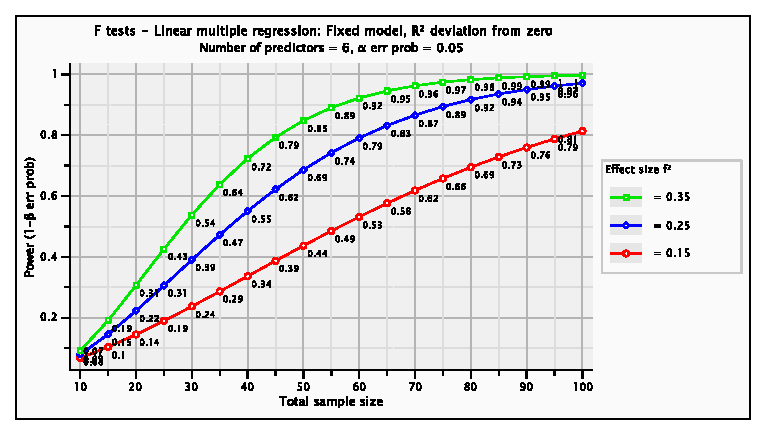
\includegraphics[width=3in]{pH}\\
  %\caption{Sample caption.}\label{label}
%\end{figure}
%\newpage
%\subsection{Multipart figures}
%For multipart figures, you need to use the package "subfig". here's an example
%\begin{verbatim}
%\begin{figure}
    %\centering
    %\subfloat[figure a]{\label{fig:figure-a} \includegraphics[width=w]{fig02a}}
    %\subfloat[figure b]{\label{fig:figure-b} \includegraphics[width=w]{fig02b}}
	%\subfloat[figure d]{\label{fig:figure-d} 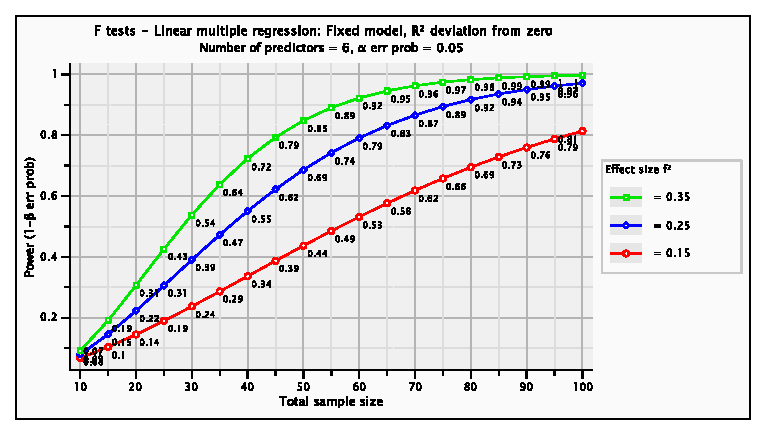
\includegraphics[width=w]{pH}}
    %\caption{Sample of a multipart figure} \label{fig:multipart-figure}
%\end{figure}
%\end{verbatim}
%\begin{figure}[h!]
    %    \centering
        %\subfloat[Circle]{\label{fig:figure-a}
\includegraphics[width=1.1in]{fig02a-circle}}
        %\subfloat[Rectangle]{\label{fig:figure-b}
\includegraphics[width=1.1in]{fig02b-rectangle}}
        %\subfloat[Cube]{\label{fig:figure-c}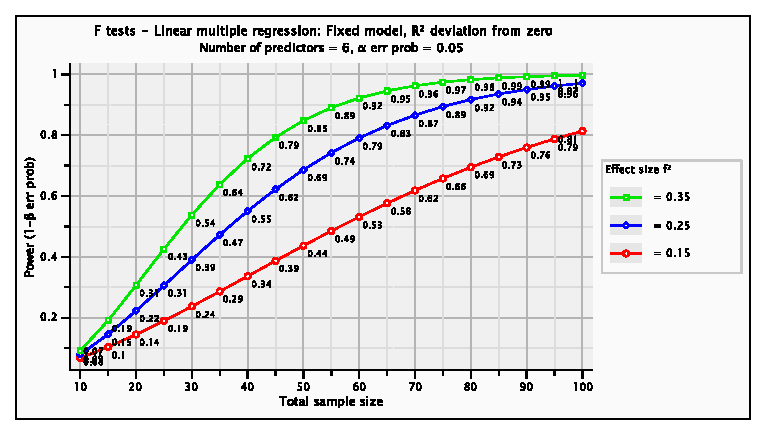
\includegraphics[width=1.1in]{pH}}
        %\caption{Geometric shapes.}
        %\label{fig:multipart-figure}
%\end{figure}
%To add some space between the figures above, one can use the usual spacing commands such as ``qquad''
%\begin{figure}[h!]
    %    \centering
        %\subfloat[Circle]{\label{fig:figure-a}
\includegraphics[width=1.1in]{fig02a-circle}} \qquad
        %\subfloat[Rectangle]{\label{fig:figure-b}
\includegraphics[width=1.1in]{fig02b-rectangle}}\qquad
        %\subfloat[Cube]{\label{fig:figure-c}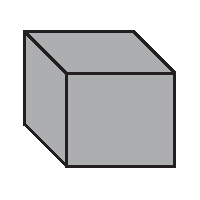
\includegraphics[width=1.1in]{fig02c-cube}}\qquad
        %\caption{Geometric shapes.}
        %\label{fig:multipart-figure}
%\end{figure} 
 
	\section{ANC}%decreasing ANC trends in Bonferoni
		  \begin{minipage}{\linewidth}
      \begin{minipage}{0.45\linewidth}
          \begin{figure}[H]
		\caption{ANC set means, class 1}
           	\begin{tikzpicture}
		\begin{axis}[xlabel = Time Set,ylabel = Means,small,xtick = {1,2,3}, ytick=data, grid=both]
		\addplot coordinates{(1,149.76) (2,173.07) (3,165.56)};
		\end{axis}
	\end{tikzpicture}
	\label{fig:ANOVAANC1}
          \end{figure}
      \end{minipage}
      \hspace{0.05\linewidth}
      \begin{minipage}{0.45\linewidth}
          \begin{figure}[H]
		\caption{ANC set means, class 2}
 		\begin{tikzpicture}
		\begin{axis}[xlabel = Time Set,ylabel = Means,small,xtick = {1,2,3}, ytick=data, grid=both]
		\addplot coordinates{(1,40.75) (2,42.20) (3,44.45)};
		\end{axis}
	\end{tikzpicture}
	\label{fig:ANOVAANC2}
          \end{figure}
      \end{minipage}
   \hspace{0.05\linewidth}
      \begin{minipage}{0.45\linewidth}
          \begin{figure}[H]
	\caption{ANC set means, class 3}
        	\begin{tikzpicture}
		\begin{axis}[xlabel = Time Set,ylabel =Means,small,xtick = {1,2,3}, ytick=data, grid=both]
		\addplot coordinates{(1,170.03) (2,172.82) (3,161.81)};
		\end{axis}
	\end{tikzpicture}
	\label{fig:ANOVAANC3}
          \end{figure}
      \end{minipage}
   \hspace{0.05\linewidth}
      \begin{minipage}{0.45\linewidth}
          \begin{figure}[H]
	\caption{ANC set means, class 4}
        \begin{tikzpicture}
		\begin{axis}[xlabel = Time Set,ylabel = Means,small,xtick = {1,2,3}, ytick=data, grid=both]
		\addplot coordinates{(1,75.52) (2,69.90) (3,64.13)};
		\end{axis}
	\end{tikzpicture}
	\label{fig:ANOVAANC4}
          \end{figure}
      \end{minipage}
   \hspace{0.05\linewidth}
      \begin{minipage}{0.45\linewidth}
          \begin{figure}[H]
	\caption{ANC set means, class 5}
        \begin{tikzpicture}
		\begin{axis}[xlabel = Time Set,ylabel =Means,small,xtick = {1,2,3}, ytick=data, grid=both]
		\addplot coordinates{(1,76.96) (2,77.84) (3,73.55)};
		\end{axis}
	\end{tikzpicture}
	\label{fig:ANOVAANC5}
          \end{figure}
      \end{minipage}
   \hspace{0.05\linewidth}
      \begin{minipage}{0.45\linewidth}
          \begin{figure}[H]
	\caption{ANC set means, class 6}
        \begin{tikzpicture}
		\begin{axis}[xlabel = Time Set,ylabel =Means,small,xtick = {1,2,3}, ytick=data, grid=both]
		\addplot coordinates{(1,68.01) (2,55.68) (3,46.80)};
		\end{axis}
	\end{tikzpicture}
	\label{fig:ANOVAANC6}
          \end{figure}
      \end{minipage}
  \end{minipage}

	\section{Nitrate}
		  \begin{minipage}{\linewidth}
      \begin{minipage}{0.45\linewidth}
          \begin{figure}[H]
           	\begin{tikzpicture}
		\begin{axis}[title=Elevation class 1, xlabel = Time Set,ylabel = Means,small,xtick = {1,2,3}]
		\addplot coordinates{(1,12.03733) (2,16.77264) (3,16.28445)};
		\end{axis}
	\end{tikzpicture}
	\label{fig:ANOVANO31}
          \end{figure}
      \end{minipage}
      \hspace{0.05\linewidth}
      \begin{minipage}{0.45\linewidth}
          \begin{figure}[H]
 		\begin{tikzpicture}
		\begin{axis}[title=Elevation class 2 , xlabel = Time Set,ylabel = Means,small,xtick = {1,2,3}]
		\addplot coordinates{(1,26.61657) (2,29.20006) (3,30.07626)};
		\end{axis}
	\end{tikzpicture}
	\label{fig:ANOVANO32}
          \end{figure}
      \end{minipage}
   \hspace{0.05\linewidth}
      \begin{minipage}{0.45\linewidth}
          \begin{figure}[H]
        	\begin{tikzpicture}
		\begin{axis}[title=Elevation class 3,xlabel = Time Set,ylabel =Means,small,xtick = {1,2,3}]
		\addplot coordinates{(1,25.97658) (2,27.68893) (3,26.17686)};
		\end{axis}
	\end{tikzpicture}
	\label{fig:ANOVANO33}
          \end{figure}
      \end{minipage}
   \hspace{0.05\linewidth}
      \begin{minipage}{0.45\linewidth}
          \begin{figure}[H]
        \begin{tikzpicture}
		\begin{axis}[title=Elevation class 4,xlabel = Time Set,ylabel = Means,small,xtick = {1,2,3}]
		\addplot coordinates{(1,12.55250) (2,17.50807) (3,18.71509)};
		\end{axis}
	\end{tikzpicture}
	\label{fig:ANOVANO34}
          \end{figure}
      \end{minipage}
   \hspace{0.05\linewidth}
      \begin{minipage}{0.45\linewidth}
          \begin{figure}[H]
        \begin{tikzpicture}
		\begin{axis}[title=Elevation class 5,xlabel = Time Set,ylabel =Means,small,xtick = {1,2,3}]
		\addplot coordinates{(1,4.35218) (2,7.43691) (3,6.44408)};
		\end{axis}
	\end{tikzpicture}
	\label{fig:ANOVANO35}
          \end{figure}
      \end{minipage}
   \hspace{0.05\linewidth}
      \begin{minipage}{0.45\linewidth}
          \begin{figure}[H]
        \begin{tikzpicture}
		\begin{axis}[title=Elevation class 6,xlabel = Time Set,ylabel =Means,small,xtick = {1,2,3}]
		\addplot coordinates{(1,21.13072) (2,24.87664) (3,31.77411)};
		\end{axis}
	\end{tikzpicture}
	\label{fig:ANOVANO36}
          \end{figure}
      \end{minipage}
  \end{minipage}

	\section{Sulfate}
		  \begin{minipage}{\linewidth}
      \begin{minipage}{0.45\linewidth}
          \begin{figure}[H]
           	\begin{tikzpicture}
		\begin{axis}[title=Elevation class 1, xlabel = Time Set,ylabel = Means,small,xtick = {1,2,3}]
		\addplot coordinates{(1,36.09) (2,39.23) (3,39.70)};
		\end{axis}
	\end{tikzpicture}
	\label{fig:ANOVASO41}
          \end{figure}
      \end{minipage}
      \hspace{0.05\linewidth}
      \begin{minipage}{0.45\linewidth}
          \begin{figure}[H]
 		\begin{tikzpicture}
		\begin{axis}[title=Elevation class 2 , xlabel = Time Set,ylabel = Means,small,xtick = {1,2,3}]
		\addplot coordinates{(1,51.68) (2,48.19) (3,47.41)};
		\end{axis}
	\end{tikzpicture}
	\label{fig:ANOVASO42}
          \end{figure}
      \end{minipage}
   \hspace{0.05\linewidth}
      \begin{minipage}{0.45\linewidth}
          \begin{figure}[H]
        	\begin{tikzpicture}
		\begin{axis}[title=Elevation class 3,xlabel = Time Set,ylabel =Means,small,xtick = {1,2,3}]
		\addplot coordinates{(1,53.98) (2,54.25) (3,58.22)};
		\end{axis}
	\end{tikzpicture}
	\label{fig:ANOVASO43}
          \end{figure}
      \end{minipage}
   \hspace{0.05\linewidth}
      \begin{minipage}{0.45\linewidth}
          \begin{figure}[H]
        \begin{tikzpicture}
		\begin{axis}[title=Elevation class 4,xlabel = Time Set,ylabel = Means,small,xtick = {1,2,3}]
		\addplot coordinates{(1,25.53) (2,29.04) (3,29.33)};
		\end{axis}
	\end{tikzpicture}
	\label{fig:ANOVASO44}
          \end{figure}
      \end{minipage}
   \hspace{0.05\linewidth}
      \begin{minipage}{0.45\linewidth}
          \begin{figure}[H]
        \begin{tikzpicture}
		\begin{axis}[title=Elevation class 5,xlabel = Time Set,ylabel =Means,small,xtick = {1,2,3}]
		\addplot coordinates{(1,27.11) (2,30.43) (3,36.16)};
		\end{axis}
	\end{tikzpicture}
	\label{fig:ANOVASO45}
          \end{figure}
      \end{minipage}
   \hspace{0.05\linewidth}
      \begin{minipage}{0.45\linewidth}
          \begin{figure}[H]
        \begin{tikzpicture}
		\begin{axis}[title=Elevation class 6,xlabel = Time Set,ylabel =Means,small,xtick = {1,2,3}]
		\addplot coordinates{(1,28.35) (2,34.31) (3,36.86)};
		\end{axis}
	\end{tikzpicture}
	\label{fig:ANOVASO46}
          \end{figure}
      \end{minipage}
  \end{minipage}


\chapter{Post Hoc Power Analsysis}\pagebreak
	\section{Step-Wise Variables}\label{sec:SWPHPA}
Post hoc power analysis using G*power and a calculated ES, $\alpha$ is .05. \textbf{Bold} results are insignificant.
		\subsection{pH}
			% Table generated by Excel2LaTeX from sheet 'Post Hoc Power analysis'
\begin{table}[htbp]
  \centering
	\caption{pH Step-Wise Post Hoc Power Analysis Results}
    \begin{tabular}{rrcrrr}
    \toprule
    Set   & Class & N     & Adjusted r$^2$ & Effect Size & Actual Power \\
    \midrule
    \multicolumn{1}{c}{\multirow{6}[1]{*}{\begin{sideways}1993-2002\end{sideways}}} & \multicolumn{1}{c}{1} & \multicolumn{1}{c}{327} & \multicolumn{1}{c}{0.712} & \multicolumn{1}{r}{2.47 } & \multicolumn{1}{c}{1.00 } \\
    \multicolumn{1}{c}{} & \multicolumn{1}{c}{2} & \multicolumn{1}{c}{393} & \multicolumn{1}{c}{0.388 } & \multicolumn{1}{r}{0.63 } & \multicolumn{1}{c}{1.00 } \\
    \multicolumn{1}{c}{} & \multicolumn{1}{c}{3} & \multicolumn{1}{c}{400} & \multicolumn{1}{c}{0.693 } & \multicolumn{1}{r}{2.26 } & \multicolumn{1}{c}{1.00 } \\
    \multicolumn{1}{c}{} & \multicolumn{1}{c}{4} & \multicolumn{1}{c}{121} & \multicolumn{1}{c}{0.205 } & \multicolumn{1}{r}{0.26 } & \multicolumn{1}{c}{0.99 } \\
    \multicolumn{1}{c}{} & \multicolumn{1}{c}{5} & \multicolumn{1}{c}{116} & \multicolumn{1}{c}{0.165 } & \multicolumn{1}{r}{0.20 } & \multicolumn{1}{c}{0.96 } \\
    \multicolumn{1}{c}{} & \multicolumn{1}{c}{6} & \multicolumn{1}{c}{110} & \multicolumn{1}{c}{0.505} & \multicolumn{1}{r}{1.02 } & \multicolumn{1}{c}{1.00 } \\\midrule
    \multicolumn{1}{c}{\multirow{6}[2]{*}{\begin{sideways}2003-2008\end{sideways}}} & \multicolumn{1}{c}{1} & \multicolumn{1}{c}{255} & \multicolumn{1}{c}{0.781 } & \multicolumn{1}{r}{3.57 } & \multicolumn{1}{c}{1.00 } \\
    \multicolumn{1}{c}{} & \multicolumn{1}{c}{2} & \multicolumn{1}{c}{289} & \multicolumn{1}{c}{0.348 } & \multicolumn{1}{r}{0.53 } & \multicolumn{1}{c}{1.00 } \\
    \multicolumn{1}{c}{} & \multicolumn{1}{c}{3} & \multicolumn{1}{c}{299} & \multicolumn{1}{c}{0.663 } & \multicolumn{1}{r}{1.97 } & \multicolumn{1}{c}{1.00 } \\
    \multicolumn{1}{c}{} & \multicolumn{1}{c}{4} & \multicolumn{1}{c}{119} & \multicolumn{1}{c}{0.400 } & \multicolumn{1}{r}{0.67 } & \multicolumn{1}{c}{1.00 } \\
    \multicolumn{1}{c}{} & \multicolumn{1}{c}{5} & \multicolumn{1}{c}{35} & \multicolumn{1}{c}{0.300 } & \multicolumn{1}{r}{0.43 } & \multicolumn{1}{c}{0.74 } \\
    \multicolumn{1}{c}{} & \multicolumn{1}{c}{6} & \multicolumn{1}{c}{97} & \multicolumn{1}{c}{0.317} & \multicolumn{1}{r}{0.46 } & \multicolumn{1}{c}{1.00 } \\\midrule
    \multicolumn{1}{c}{\multirow{6}[2]{*}{\begin{sideways}2009-2012\end{sideways}}} & \multicolumn{1}{c}{1} & \multicolumn{1}{c}{191} & \multicolumn{1}{c}{0.894 } & \multicolumn{1}{r}{8.43 } & \multicolumn{1}{c}{1.00 } \\
    \multicolumn{1}{c}{} & \multicolumn{1}{c}{2} & \multicolumn{1}{c}{212} & \multicolumn{1}{c}{0.606 } & \multicolumn{1}{r}{1.54 } & \multicolumn{1}{c}{1.00 } \\
    \multicolumn{1}{c}{} & \multicolumn{1}{c}{3} & \multicolumn{1}{c}{228} & \multicolumn{1}{c}{0.766 } & \multicolumn{1}{r}{3.27 } & \multicolumn{1}{c}{1.00 } \\
    \multicolumn{1}{c}{} & \multicolumn{1}{c}{4} & \multicolumn{1}{c}{97} & \multicolumn{1}{c}{0.593 } & \multicolumn{1}{r}{1.46 } & \multicolumn{1}{c}{1.00 } \\
    \multicolumn{1}{c}{} & \multicolumn{1}{c}{5} & \multicolumn{1}{c}{29} & \multicolumn{1}{c}{\textbf{0.158 }} & \multicolumn{1}{r}{0.19 } & \multicolumn{1}{c}{0.28 } \\
    \multicolumn{1}{c}{} & \multicolumn{1}{c}{6} & \multicolumn{1}{c}{76} & \multicolumn{1}{c}{0.286} & \multicolumn{1}{r}{0.40 } & \multicolumn{1}{c}{0.99 } \\
    \bottomrule
    \end{tabular}%
  \label{tab:pHSWPHPA}%
\end{table}%
\pagebreak%needs cleaning

		\subsection{ANC}
			% Table generated by Excel2LaTeX from sheet 'Post Hoc Power analysis'
\begin{table}[htbp]
  \centering
	\caption{ANC Step-Wise Post Hoc Power Analysis Results}
    \begin{tabular}{rrcrrr}
    \toprule
    Set   & Class & N     & Adjusted r$^2$ & Effect Size & Actual Power \\
    \midrule
    \multicolumn{1}{c}{\multirow{6}[1]{*}{\begin{sideways}1993-2002\end{sideways}}} & \multicolumn{1}{c}{1} & \multicolumn{1}{c}{327} & \multicolumn{1}{c}{0.985 } & \multicolumn{1}{r}{65.67 } & \multicolumn{1}{c}{1.00 } \\
    \multicolumn{1}{c}{} & \multicolumn{1}{c}{2} & \multicolumn{1}{c}{392} & \multicolumn{1}{c}{0.603 } & \multicolumn{1}{r}{1.52 } & \multicolumn{1}{c}{1.00 } \\
    \multicolumn{1}{c}{} & \multicolumn{1}{c}{3} & \multicolumn{1}{c}{398} & \multicolumn{1}{c}{0.971 } & \multicolumn{1}{r}{33.48 } & \multicolumn{1}{c}{1.00 } \\
    \multicolumn{1}{c}{} & \multicolumn{1}{c}{4} & \multicolumn{1}{c}{120} & \multicolumn{1}{c}{0.709 } & \multicolumn{1}{r}{2.44 } & \multicolumn{1}{c}{1.00 } \\
    \multicolumn{1}{c}{} & \multicolumn{1}{c}{5} & \multicolumn{1}{c}{116} & \multicolumn{1}{c}{0.760 } & \multicolumn{1}{r}{3.17 } & \multicolumn{1}{c}{1.00 } \\
    \multicolumn{1}{c}{} & \multicolumn{1}{c}{6} & \multicolumn{1}{c}{110} & \multicolumn{1}{c}{0.802} & \multicolumn{1}{r}{4.05 } & \multicolumn{1}{c}{1.00 } \\\midrule
    \multicolumn{1}{c}{\multirow{6}[2]{*}{\begin{sideways}2003-2008\end{sideways}}} & \multicolumn{1}{c}{1} & \multicolumn{1}{c}{255} & \multicolumn{1}{c}{0.996 } & \multicolumn{1}{r}{249.00 } & \multicolumn{1}{c}{1.00 } \\
    \multicolumn{1}{c}{} & \multicolumn{1}{c}{2} & \multicolumn{1}{c}{289} & \multicolumn{1}{c}{0.779 } & \multicolumn{1}{r}{3.52 } & \multicolumn{1}{c}{1.00 } \\
    \multicolumn{1}{c}{} & \multicolumn{1}{c}{3} & \multicolumn{1}{c}{299} & \multicolumn{1}{c}{0.996 } & \multicolumn{1}{r}{249.00 } & \multicolumn{1}{c}{1.00 } \\
    \multicolumn{1}{c}{} & \multicolumn{1}{c}{4} & \multicolumn{1}{c}{119} & \multicolumn{1}{c}{0.779 } & \multicolumn{1}{r}{3.52 } & \multicolumn{1}{c}{1.00 } \\
    \multicolumn{1}{c}{} & \multicolumn{1}{c}{5} & \multicolumn{1}{c}{35} & \multicolumn{1}{c}{0.739 } & \multicolumn{1}{r}{2.83 } & \multicolumn{1}{c}{1.00 } \\
    \multicolumn{1}{c}{} & \multicolumn{1}{c}{6} & \multicolumn{1}{c}{97} & \multicolumn{1}{c}{0.812} & \multicolumn{1}{r}{4.32 } & \multicolumn{1}{c}{1.00 } \\\midrule
    \multicolumn{1}{c}{\multirow{6}[2]{*}{\begin{sideways}2009-2012\end{sideways}}} & \multicolumn{1}{c}{1} & \multicolumn{1}{c}{191} & \multicolumn{1}{c}{0.989 } & \multicolumn{1}{r}{89.91 } & \multicolumn{1}{c}{1.00 } \\
    \multicolumn{1}{c}{} & \multicolumn{1}{c}{2} & \multicolumn{1}{c}{212} & \multicolumn{1}{c}{0.862 } & \multicolumn{1}{r}{6.25 } & \multicolumn{1}{c}{1.00 } \\
    \multicolumn{1}{c}{} & \multicolumn{1}{c}{3} & \multicolumn{1}{c}{228} & \multicolumn{1}{c}{0.997 } & \multicolumn{1}{r}{332.33 } & \multicolumn{1}{c}{1.00 } \\
    \multicolumn{1}{c}{} & \multicolumn{1}{c}{4} & \multicolumn{1}{c}{97} & \multicolumn{1}{c}{0.772 } & \multicolumn{1}{r}{3.39 } & \multicolumn{1}{c}{1.00 } \\
    \multicolumn{1}{c}{} & \multicolumn{1}{c}{5} & \multicolumn{1}{c}{29} & \multicolumn{1}{c}{0.540 } & \multicolumn{1}{r}{1.17 } & \multicolumn{1}{c}{0.96 } \\
    \multicolumn{1}{c}{} & \multicolumn{1}{c}{6} & \multicolumn{1}{c}{76} & \multicolumn{1}{c}{0.809} & \multicolumn{1}{r}{4.24 } & \multicolumn{1}{c}{1.00 } \\
    \bottomrule
    \end{tabular}%
  \label{tab:ANCSWPHPA}%
\end{table}%
\pagebreak

		\subsection{NO3}
			% Table generated by Excel2LaTeX from sheet 'Post Hoc Power analysis'
\begin{table}[htbp]
  \centering
	\caption{Nitrate Step-Wise Post Hoc Power Analysis Results}
    \begin{tabular}{rrcrrr}
    \toprule
    Set   & Class & N     & Adjusted r$^2$ & Effect Size & Actual Power \\
    \midrule
    \multicolumn{1}{c}{\multirow{6}[1]{*}{\begin{sideways}1993-2002\end{sideways}}} & \multicolumn{1}{c}{1} & \multicolumn{1}{c}{275} & \multicolumn{1}{c}{0.503 } & \multicolumn{1}{r}{1.01 } & \multicolumn{1}{c}{1.00 } \\
    \multicolumn{1}{c}{} & \multicolumn{1}{c}{2} & \multicolumn{1}{c}{377} & \multicolumn{1}{c}{0.699 } & \multicolumn{1}{r}{2.32 } & \multicolumn{1}{c}{1.00 } \\
    \multicolumn{1}{c}{} & \multicolumn{1}{c}{3} & \multicolumn{1}{c}{365} & \multicolumn{1}{c}{0.359 } & \multicolumn{1}{r}{0.56 } & \multicolumn{1}{c}{1.00 } \\
    \multicolumn{1}{c}{} & \multicolumn{1}{c}{4} & \multicolumn{1}{c}{105} & \multicolumn{1}{c}{0.410 } & \multicolumn{1}{r}{0.69 } & \multicolumn{1}{c}{1.00 } \\
    \multicolumn{1}{c}{} & \multicolumn{1}{c}{5} & \multicolumn{1}{c}{66} & \multicolumn{1}{c}{0.328 } & \multicolumn{1}{r}{0.49 } & \multicolumn{1}{c}{0.98 } \\
    \multicolumn{1}{c}{} & \multicolumn{1}{c}{6} & \multicolumn{1}{c}{81} & \multicolumn{1}{c}{0.871 } & \multicolumn{1}{r}{6.75 } & \multicolumn{1}{c}{1.00 } \\\midrule
    \multicolumn{1}{c}{\multirow{6}[2]{*}{\begin{sideways}2003-2008\end{sideways}}} & \multicolumn{1}{c}{1} & \multicolumn{1}{c}{252} & \multicolumn{1}{c}{0.551 } & \multicolumn{1}{r}{1.23 } & \multicolumn{1}{c}{1.00 } \\
    \multicolumn{1}{c}{} & \multicolumn{1}{c}{2} & \multicolumn{1}{c}{296} & \multicolumn{1}{c}{0.816 } & \multicolumn{1}{r}{4.43 } & \multicolumn{1}{c}{1.00 } \\
    \multicolumn{1}{c}{} & \multicolumn{1}{c}{3} & \multicolumn{1}{c}{297} & \multicolumn{1}{c}{0.637 } & \multicolumn{1}{r}{1.75 } & \multicolumn{1}{c}{1.00 } \\
    \multicolumn{1}{c}{} & \multicolumn{1}{c}{4} & \multicolumn{1}{c}{121} & \multicolumn{1}{c}{0.405 } & \multicolumn{1}{r}{0.68 } & \multicolumn{1}{c}{1.00 } \\
    \multicolumn{1}{c}{} & \multicolumn{1}{c}{5} & \multicolumn{1}{c}{30} & \multicolumn{1}{c}{0.562 } & \multicolumn{1}{r}{1.28 } & \multicolumn{1}{c}{0.98 } \\
    \multicolumn{1}{c}{} & \multicolumn{1}{c}{6} & \multicolumn{1}{c}{98} & \multicolumn{1}{c}{0.832 } & \multicolumn{1}{r}{4.95 } & \multicolumn{1}{c}{1.00 } \\\midrule
    \multicolumn{1}{c}{\multirow{6}[2]{*}{\begin{sideways}2009-2012\end{sideways}}} & \multicolumn{1}{c}{1} & \multicolumn{1}{c}{191} & \multicolumn{1}{c}{0.376 } & \multicolumn{1}{r}{0.60 } & \multicolumn{1}{c}{1.00 } \\
    \multicolumn{1}{c}{} & \multicolumn{1}{c}{2} & \multicolumn{1}{c}{212} & \multicolumn{1}{c}{0.735 } & \multicolumn{1}{r}{2.77 } & \multicolumn{1}{c}{1.00 } \\
    \multicolumn{1}{c}{} & \multicolumn{1}{c}{3} & \multicolumn{1}{c}{228} & \multicolumn{1}{c}{0.598 } & \multicolumn{1}{r}{1.49 } & \multicolumn{1}{c}{1.00 } \\
    \multicolumn{1}{c}{} & \multicolumn{1}{c}{4} & \multicolumn{1}{c}{97} & \multicolumn{1}{c}{0.635 } & \multicolumn{1}{r}{1.74 } & \multicolumn{1}{c}{1.00 } \\
    \multicolumn{1}{c}{} & \multicolumn{1}{c}{5} & \multicolumn{1}{c}{29} & \multicolumn{1}{c}{\textbf{-0.272 }} & \multicolumn{1}{r}{NA} & \multicolumn{1}{c}{NA} \\
    \multicolumn{1}{c}{} & \multicolumn{1}{c}{6} & \multicolumn{1}{c}{76} & \multicolumn{1}{c}{0.881 } & \multicolumn{1}{r}{7.40 } & \multicolumn{1}{c}{1.00 } \\
    \bottomrule
    \end{tabular}%
  \label{tab:NO3SWPHPA}%
\end{table}%
\pagebreak

		\subsection{SO4}
			% Table generated by Excel2LaTeX from sheet 'Post Hoc Power analysis'
\begin{table}[htbp]
  \centering
	  \caption{Sulfate Step-Wise Post Hoc Power Analysis Results}
    \begin{tabular}{rrcrrr}
    \toprule
    Set   & Class & N     & Adjusted r$^2$ & Effect Size & Actual Power \\
    \midrule
    \multicolumn{1}{c}{\multirow{6}[1]{*}{\begin{sideways}1993-2002\end{sideways}}} & \multicolumn{1}{c}{1} & \multicolumn{1}{c}{325} & \multicolumn{1}{c}{0.569 } & \multicolumn{1}{r}{1.32 } & \multicolumn{1}{c}{1.00 } \\
    \multicolumn{1}{c}{} & \multicolumn{1}{c}{2} & \multicolumn{1}{c}{390} & \multicolumn{1}{c}{0.766 } & \multicolumn{1}{r}{3.27 } & \multicolumn{1}{c}{1.00 } \\
    \multicolumn{1}{c}{} & \multicolumn{1}{c}{3} & \multicolumn{1}{c}{391} & \multicolumn{1}{c}{0.590 } & \multicolumn{1}{r}{1.44 } & \multicolumn{1}{c}{1.00 } \\
    \multicolumn{1}{c}{} & \multicolumn{1}{c}{4} & \multicolumn{1}{c}{119} & \multicolumn{1}{c}{0.402 } & \multicolumn{1}{r}{0.67 } & \multicolumn{1}{c}{1.00 } \\
    \multicolumn{1}{c}{} & \multicolumn{1}{c}{5} & \multicolumn{1}{c}{116} & \multicolumn{1}{c}{0.566 } & \multicolumn{1}{r}{1.30 } & \multicolumn{1}{c}{1.00 } \\
    \multicolumn{1}{c}{} & \multicolumn{1}{c}{6} & \multicolumn{1}{c}{110} & \multicolumn{1}{c}{0.716 } & \multicolumn{1}{r}{2.52 } & \multicolumn{1}{c}{1.00 } \\\midrule
    \multicolumn{1}{c}{\multirow{6}[2]{*}{\begin{sideways}2003-2008\end{sideways}}} & \multicolumn{1}{c}{1} & \multicolumn{1}{c}{261} & \multicolumn{1}{c}{0.673 } & \multicolumn{1}{r}{2.06 } & \multicolumn{1}{c}{1.00 } \\
    \multicolumn{1}{c}{} & \multicolumn{1}{c}{2} & \multicolumn{1}{c}{298} & \multicolumn{1}{c}{0.893 } & \multicolumn{1}{r}{8.35 } & \multicolumn{1}{c}{1.00 } \\
    \multicolumn{1}{c}{} & \multicolumn{1}{c}{3} & \multicolumn{1}{c}{308} & \multicolumn{1}{c}{0.923 } & \multicolumn{1}{r}{11.99 } & \multicolumn{1}{c}{1.00 } \\
    \multicolumn{1}{c}{} & \multicolumn{1}{c}{4} & \multicolumn{1}{c}{123} & \multicolumn{1}{c}{0.343 } & \multicolumn{1}{r}{0.52 } & \multicolumn{1}{c}{1.00 } \\
    \multicolumn{1}{c}{} & \multicolumn{1}{c}{5} & \multicolumn{1}{c}{37} & \multicolumn{1}{c}{0.884 } & \multicolumn{1}{r}{7.62 } & \multicolumn{1}{c}{1.00 } \\
    \multicolumn{1}{c}{} & \multicolumn{1}{c}{6} & \multicolumn{1}{c}{101} & \multicolumn{1}{c}{0.844 } & \multicolumn{1}{r}{5.41 } & \multicolumn{1}{c}{1.00 } \\\midrule
    \multicolumn{1}{c}{\multirow{6}[2]{*}{\begin{sideways}2009-2012\end{sideways}}} & \multicolumn{1}{c}{1} & \multicolumn{1}{r}{190} & \multicolumn{1}{c}{0.536 } & \multicolumn{1}{r}{1.16 } & \multicolumn{1}{c}{1.00 } \\
    \multicolumn{1}{c}{} & \multicolumn{1}{c}{2} & \multicolumn{1}{c}{212} & \multicolumn{1}{c}{0.887 } & \multicolumn{1}{r}{7.85 } & \multicolumn{1}{c}{1.00 } \\
    \multicolumn{1}{c}{} & \multicolumn{1}{c}{3} & \multicolumn{1}{c}{228} & \multicolumn{1}{c}{0.915 } & \multicolumn{1}{r}{10.76 } & \multicolumn{1}{c}{1.00 } \\
    \multicolumn{1}{c}{} & \multicolumn{1}{c}{4} & \multicolumn{1}{c}{97} & \multicolumn{1}{c}{0.529 } & \multicolumn{1}{r}{1.12 } & \multicolumn{1}{c}{1.00 } \\
    \multicolumn{1}{c}{} & \multicolumn{1}{c}{5} & \multicolumn{1}{c}{29} & \multicolumn{1}{c}{0.658 } & \multicolumn{1}{r}{1.92 } & \multicolumn{1}{c}{1.00 } \\
    \multicolumn{1}{c}{} & \multicolumn{1}{c}{6} & \multicolumn{1}{c}{76} & \multicolumn{1}{c}{0.861 } & \multicolumn{1}{r}{6.19 } & \multicolumn{1}{c}{1.00 } \\
    \bottomrule
    \end{tabular}%
  \label{tab:SO4SWPHPA}%
\end{table}%
\pagebreak


	\section{Temperol variables}\label{sec:TVPHPA}
Post hoc power analysis using G*power a calculated ES, an alpha of .05 with the variables: $\sin(\theta)$, $\cos(\theta)$, and Julian date only.   \textbf{Bold} results are insignificant.
		\subsection{pH}
			% Table generated by Excel2LaTeX from sheet 'Post Hoc Power analysis'
\begin{table}[htbp]
  \centering
  \caption{pH Time Variable Post Hoc Power Analysis Results}
    \begin{tabular}{rrrrrr}
    \toprule
    Set   & Class & N     & Adjusted r$^2$ & Effect Size & Actual Power \\
    \midrule
    \multicolumn{1}{c}{\multirow{6}[1]{*}{\begin{sideways}1993-2002\end{sideways}}} & \multicolumn{1}{c}{1} & \multicolumn{1}{c}{327} & \multicolumn{1}{c}{\textbf{0.047 }} & \multicolumn{1}{c}{0.049 } & \multicolumn{1}{c}{0.93 } \\
    \multicolumn{1}{c}{} & \multicolumn{1}{c}{2} & \multicolumn{1}{c}{393} & \multicolumn{1}{c}{\textbf{0.128 }} & \multicolumn{1}{c}{0.15 } & \multicolumn{1}{c}{1.00 } \\
    \multicolumn{1}{c}{} & \multicolumn{1}{c}{3} & \multicolumn{1}{c}{400} & \multicolumn{1}{c}{\textbf{0.013 }} & \multicolumn{1}{c}{0.01 } & \multicolumn{1}{c}{0.46 } \\
    \multicolumn{1}{c}{} & \multicolumn{1}{c}{4} & \multicolumn{1}{c}{121} & \multicolumn{1}{c}{\textbf{0.059 }} & \multicolumn{1}{c}{0.06 } & \multicolumn{1}{c}{0.61 } \\
    \multicolumn{1}{c}{} & \multicolumn{1}{c}{5} & \multicolumn{1}{c}{116} & \multicolumn{1}{c}{\textbf{0.051 }} & \multicolumn{1}{c}{0.05 } & \multicolumn{1}{c}{0.52 } \\
    \multicolumn{1}{c}{} & \multicolumn{1}{c}{6} & \multicolumn{1}{c}{110} & \multicolumn{1}{c}{\textbf{0.096 }} & \multicolumn{1}{c}{0.11 } & \multicolumn{1}{c}{0.81 } \\\midrule
    \multicolumn{1}{c}{\multirow{6}[2]{*}{\begin{sideways}2003-2008\end{sideways}}} & \multicolumn{1}{c}{1} & \multicolumn{1}{c}{255} & \multicolumn{1}{c}{0.040 } & \multicolumn{1}{c}{0.04 } & \multicolumn{1}{c}{0.78 } \\
    \multicolumn{1}{c}{} & \multicolumn{1}{c}{2} & \multicolumn{1}{c}{289} & \multicolumn{1}{c}{0.061 } & \multicolumn{1}{c}{0.06 } & \multicolumn{1}{c}{0.96 } \\
    \multicolumn{1}{c}{} & \multicolumn{1}{c}{3} & \multicolumn{1}{c}{299} & \multicolumn{1}{c}{\textbf{0.020 }} & \multicolumn{1}{c}{0.02 } & \multicolumn{1}{c}{0.52 } \\
    \multicolumn{1}{c}{} & \multicolumn{1}{c}{4} & \multicolumn{1}{c}{119} & \multicolumn{1}{c}{0.148 } & \multicolumn{1}{c}{0.17 } & \multicolumn{1}{c}{0.97 } \\
    \multicolumn{1}{c}{} & \multicolumn{1}{c}{5} & \multicolumn{1}{c}{35} & \multicolumn{1}{c}{\textbf{-0.069 }} & \multicolumn{1}{c}{NA} & \multicolumn{1}{c}{NA} \\
    \multicolumn{1}{c}{} & \multicolumn{1}{c}{6} & \multicolumn{1}{c}{97} & \multicolumn{1}{c}{0.081 } & \multicolumn{1}{c}{0.09 } & \multicolumn{1}{c}{0.67 } \\\midrule
    \multicolumn{1}{c}{\multirow{6}[2]{*}{\begin{sideways}2009-2012\end{sideways}}} & \multicolumn{1}{c}{1} & \multicolumn{1}{c}{191} & \multicolumn{1}{c}{\textbf{0.028 }} & \multicolumn{1}{c}{0.03 } & \multicolumn{1}{c}{0.47 } \\
    \multicolumn{1}{c}{} & \multicolumn{1}{c}{2} & \multicolumn{1}{c}{212} & \multicolumn{1}{c}{0.052 } & \multicolumn{1}{c}{0.05 } & \multicolumn{1}{c}{0.82 } \\
    \multicolumn{1}{c}{} & \multicolumn{1}{c}{3} & \multicolumn{1}{c}{228} & \multicolumn{1}{c}{\textbf{-0.009 }} & \multicolumn{1}{c}{NA} & \multicolumn{1}{c}{NA} \\
    \multicolumn{1}{c}{} & \multicolumn{1}{c}{4} & \multicolumn{1}{c}{97} & \multicolumn{1}{c}{0.200 } & \multicolumn{1}{c}{0.25 } & \multicolumn{1}{c}{0.99 } \\
    \multicolumn{1}{c}{} & \multicolumn{1}{c}{5} & \multicolumn{1}{c}{29} & \multicolumn{1}{c}{\textbf{0.218 }} & \multicolumn{1}{c}{0.28 } & \multicolumn{1}{c}{0.58 } \\
    \multicolumn{1}{c}{} & \multicolumn{1}{c}{6} & \multicolumn{1}{c}{76} & \multicolumn{1}{c}{0.039 } & \multicolumn{1}{c}{0.04 } & \multicolumn{1}{c}{0.27 } \\
    \bottomrule
    \end{tabular}%
  \label{tab:pHTVPHPA}%
\end{table}%
\pagebreak%needs cleaning

		\subsection{ANC}
			% Table generated by Excel2LaTeX from sheet 'Post Hoc Power analysis'
\begin{table}[htbp]
  \centering
	  \caption{ANC Time Variable Post Hoc Power Analysis Results}
    \begin{tabular}{rrrrrr}
    \toprule
    Set   & Class & N     & Adjusted r$^2$ & Effect Size & Actual Power \\
    \midrule
    \multicolumn{1}{c}{\multirow{6}[1]{*}{\begin{sideways}1993-2002\end{sideways}}} & \multicolumn{1}{c}{1} & \multicolumn{1}{c}{327} & \multicolumn{1}{c}{\textbf{0.024 }} & \multicolumn{1}{c}{0.02 } & \multicolumn{1}{c}{0.65 } \\
    \multicolumn{1}{c}{} & \multicolumn{1}{c}{2} & \multicolumn{1}{c}{392} & \multicolumn{1}{c}{\textbf{0.189 }} & \multicolumn{1}{c}{0.23 } & \multicolumn{1}{c}{1.00 } \\
    \multicolumn{1}{c}{} & \multicolumn{1}{c}{3} & \multicolumn{1}{c}{398} & \multicolumn{1}{c}{\textbf{0.000 }} & \multicolumn{1}{c}{0.00 } & \multicolumn{1}{c}{0.06 } \\
    \multicolumn{1}{c}{} & \multicolumn{1}{c}{4} & \multicolumn{1}{c}{120} & \multicolumn{1}{c}{\textbf{0.294 }} & \multicolumn{1}{c}{0.42 } & \multicolumn{1}{c}{1.00 } \\
    \multicolumn{1}{c}{} & \multicolumn{1}{c}{5} & \multicolumn{1}{c}{116} & \multicolumn{1}{c}{0.381 } & \multicolumn{1}{c}{0.62 } & \multicolumn{1}{c}{1.00 } \\
    \multicolumn{1}{c}{} & \multicolumn{1}{c}{6} & \multicolumn{1}{c}{110} & \multicolumn{1}{c}{\textbf{0.075 }} & \multicolumn{1}{c}{0.08 } & \multicolumn{1}{c}{0.69 } \\\midrule
    \multicolumn{1}{c}{\multirow{6}[2]{*}{\begin{sideways}2003-2008\end{sideways}}} & \multicolumn{1}{c}{1} & \multicolumn{1}{c}{255} & \multicolumn{1}{c}{\textbf{0.001 }} & \multicolumn{1}{c}{0.00 } & \multicolumn{1}{c}{0.07 } \\
    \multicolumn{1}{c}{} & \multicolumn{1}{c}{2} & \multicolumn{1}{c}{289} & \multicolumn{1}{c}{\textbf{0.081 }} & \multicolumn{1}{c}{0.09 } & \multicolumn{1}{c}{0.99 } \\
    \multicolumn{1}{c}{} & \multicolumn{1}{c}{3} & \multicolumn{1}{c}{299} & \multicolumn{1}{c}{\textbf{-0.003 }} & \multicolumn{1}{c}{NA} & \multicolumn{1}{c}{NA} \\
    \multicolumn{1}{c}{} & \multicolumn{1}{c}{4} & \multicolumn{1}{c}{119} & \multicolumn{1}{c}{\textbf{0.180 }} & \multicolumn{1}{c}{0.22 } & \multicolumn{1}{c}{0.99 } \\
    \multicolumn{1}{c}{} & \multicolumn{1}{c}{5} & \multicolumn{1}{c}{35} & \multicolumn{1}{c}{\textbf{0.337 }} & \multicolumn{1}{c}{0.51 } & \multicolumn{1}{c}{0.93 } \\
    \multicolumn{1}{c}{} & \multicolumn{1}{c}{6} & \multicolumn{1}{c}{97} & \multicolumn{1}{c}{\textbf{0.094 }} & \multicolumn{1}{c}{0.10 } & \multicolumn{1}{c}{0.74 } \\\midrule
    \multicolumn{1}{c}{\multirow{6}[2]{*}{\begin{sideways}2009-2012\end{sideways}}} & \multicolumn{1}{c}{1} & \multicolumn{1}{c}{191} & \multicolumn{1}{c}{\textbf{0.000 }} & \multicolumn{1}{c}{0.00 } & \multicolumn{1}{c}{0.05 } \\
    \multicolumn{1}{c}{} & \multicolumn{1}{c}{2} & \multicolumn{1}{c}{212} & \multicolumn{1}{c}{\textbf{0.056 }} & \multicolumn{1}{c}{0.06 } & \multicolumn{1}{c}{0.85 } \\
    \multicolumn{1}{c}{} & \multicolumn{1}{c}{3} & \multicolumn{1}{c}{228} & \multicolumn{1}{c}{\textbf{-0.002 }} & \multicolumn{1}{c}{NA} & \multicolumn{1}{c}{NA} \\
    \multicolumn{1}{c}{} & \multicolumn{1}{c}{4} & \multicolumn{1}{c}{97} & \multicolumn{1}{c}{\textbf{0.161 }} & \multicolumn{1}{c}{0.19 } & \multicolumn{1}{c}{0.96 } \\
    \multicolumn{1}{c}{} & \multicolumn{1}{c}{5} & \multicolumn{1}{c}{29} & \multicolumn{1}{c}{0.466 } & \multicolumn{1}{c}{0.87 } & \multicolumn{1}{c}{0.98 } \\
    \multicolumn{1}{c}{} & \multicolumn{1}{c}{6} & \multicolumn{1}{c}{76} & \multicolumn{1}{c}{\textbf{0.058 }} & \multicolumn{1}{c}{0.06 } & \multicolumn{1}{c}{0.39 } \\
    \bottomrule
    \end{tabular}%
  \label{tab:ANCTVPHPA}%
\end{table}%
\pagebreak

		\subsection{NO3}
			% Table generated by Excel2LaTeX from sheet 'Post Hoc Power analysis'
\begin{table}[htbp]
  \centering
  \caption{Nitrate Time Variable Post Hoc Power Analysis Results}
    \begin{tabular}{rrrrrr}
    \toprule
    Set   & Class & N     & Adjusted r$^2$ & Effect Size & Actual Power \\
    \midrule
    \multicolumn{1}{c}{\multirow{6}[1]{*}{\begin{sideways}1993-2002\end{sideways}}} & \multicolumn{1}{c}{1} & \multicolumn{1}{c}{275} & \multicolumn{1}{c}{0.016 } & \multicolumn{1}{c}{0.02 } & \multicolumn{1}{c}{0.39 } \\
    \multicolumn{1}{c}{} & \multicolumn{1}{c}{2} & \multicolumn{1}{c}{377} & \multicolumn{1}{c}{\textbf{0.017 }} & \multicolumn{1}{c}{0.02 } & \multicolumn{1}{c}{0.55 } \\
    \multicolumn{1}{c}{} & \multicolumn{1}{c}{3} & \multicolumn{1}{c}{365} & \multicolumn{1}{c}{\textbf{-0.004 }} & \multicolumn{1}{c}{NA} & \multicolumn{1}{c}{NA} \\
    \multicolumn{1}{c}{} & \multicolumn{1}{c}{4} & \multicolumn{1}{c}{105} & \multicolumn{1}{c}{\textbf{-0.027 }} & \multicolumn{1}{c}{NA} & \multicolumn{1}{c}{NA} \\
    \multicolumn{1}{c}{} & \multicolumn{1}{c}{5} & \multicolumn{1}{c}{66} & \multicolumn{1}{c}{0.120 } & \multicolumn{1}{c}{0.14 } & \multicolumn{1}{c}{0.68 } \\
    \multicolumn{1}{c}{} & \multicolumn{1}{c}{6} & \multicolumn{1}{c}{81} & \multicolumn{1}{c}{\textbf{0.092 }} & \multicolumn{1}{c}{0.10 } & \multicolumn{1}{c}{0.64 } \\\midrule
    \multicolumn{1}{c}{\multirow{6}[2]{*}{\begin{sideways}2003-2008\end{sideways}}} & \multicolumn{1}{c}{1} & \multicolumn{1}{c}{252} & \multicolumn{1}{c}{0.061 } & \multicolumn{1}{c}{0.06 } & \multicolumn{1}{c}{0.94 } \\
    \multicolumn{1}{c}{} & \multicolumn{1}{c}{2} & \multicolumn{1}{c}{296} & \multicolumn{1}{c}{0.043 } & \multicolumn{1}{c}{0.04 } & \multicolumn{1}{c}{0.87 } \\
    \multicolumn{1}{c}{} & \multicolumn{1}{c}{3} & \multicolumn{1}{c}{297} & \multicolumn{1}{c}{\textbf{-0.003 }} & \multicolumn{1}{c}{NA} & \multicolumn{1}{c}{NA} \\
    \multicolumn{1}{c}{} & \multicolumn{1}{c}{4} & \multicolumn{1}{c}{121} & \multicolumn{1}{c}{0.086 } & \multicolumn{1}{c}{0.09 } & \multicolumn{1}{c}{0.80 } \\
    \multicolumn{1}{c}{} & \multicolumn{1}{c}{5} & \multicolumn{1}{c}{30} & \multicolumn{1}{c}{\textbf{-0.082 }} & \multicolumn{1}{c}{NA} & \multicolumn{1}{c}{NA} \\
    \multicolumn{1}{c}{} & \multicolumn{1}{c}{6} & \multicolumn{1}{c}{98} & \multicolumn{1}{c}{0.046 } & \multicolumn{1}{c}{0.05 } & \multicolumn{1}{c}{0.40 } \\\midrule
    \multicolumn{1}{c}{\multirow{6}[2]{*}{\begin{sideways}2009-2012\end{sideways}}} & \multicolumn{1}{c}{1} & \multicolumn{1}{c}{191} & \multicolumn{1}{c}{\textbf{0.018 }} & \multicolumn{1}{c}{0.02 } & \multicolumn{1}{c}{0.31 } \\
    \multicolumn{1}{c}{} & \multicolumn{1}{c}{2} & \multicolumn{1}{c}{212} & \multicolumn{1}{c}{\textbf{0.011 }} & \multicolumn{1}{c}{0.01 } & \multicolumn{1}{c}{0.22 } \\
    \multicolumn{1}{c}{} & \multicolumn{1}{c}{3} & \multicolumn{1}{c}{228} & \multicolumn{1}{c}{\textbf{-0.004 }} & \multicolumn{1}{c}{NA} & \multicolumn{1}{c}{NA} \\
    \multicolumn{1}{c}{} & \multicolumn{1}{c}{4} & \multicolumn{1}{c}{97} & \multicolumn{1}{c}{\textbf{-0.016 }} & \multicolumn{1}{c}{NA} & \multicolumn{1}{c}{NA} \\
    \multicolumn{1}{c}{} & \multicolumn{1}{c}{5} & \multicolumn{1}{c}{29} & \multicolumn{1}{c}{\textbf{-0.039 }} & \multicolumn{1}{c}{NA} & \multicolumn{1}{c}{NA} \\
    \multicolumn{1}{c}{} & \multicolumn{1}{c}{6} & \multicolumn{1}{c}{76} & \multicolumn{1}{c}{\textbf{-0.016 }} & \multicolumn{1}{c}{NA} & \multicolumn{1}{c}{NA} \\
    \bottomrule
    \end{tabular}%
  \label{tab:NO3TVPHPA}%
\end{table}%
\pagebreak

		\subsection{SO4}
			% Table generated by Excel2LaTeX from sheet 'Post Hoc Power analysis'
\begin{table}[htbp]
  \centering
  \caption{Sulfate Time Variable Post Hoc Power Analysis Results}
    \begin{tabular}{rrrrrr}
    \toprule
    Set   & Class & N     & Adjusted r$^2$ & Effect Size & Actual Power \\
    \midrule
    \multicolumn{1}{c}{\multirow{6}[1]{*}{\begin{sideways}1993-2002\end{sideways}}} & \multicolumn{1}{c}{1} & \multicolumn{1}{c}{325} & \multicolumn{1}{c}{0.045 } & \multicolumn{1}{c}{0.05 } & \multicolumn{1}{c}{0.92 } \\
    \multicolumn{1}{c}{} & \multicolumn{1}{c}{2} & \multicolumn{1}{c}{390} & \multicolumn{1}{c}{\textbf{0.009 }} & \multicolumn{1}{c}{0.01 } & \multicolumn{1}{c}{0.32 } \\
    \multicolumn{1}{c}{} & \multicolumn{1}{c}{3} & \multicolumn{1}{c}{391} & \multicolumn{1}{c}{\textbf{-0.004 }} & \multicolumn{1}{c}{ NA} & \multicolumn{1}{c}{NA} \\
    \multicolumn{1}{c}{} & \multicolumn{1}{c}{4} & \multicolumn{1}{c}{119} & \multicolumn{1}{c}{\textbf{-0.016 }} & \multicolumn{1}{c}{NA} & \multicolumn{1}{c}{NA} \\
    \multicolumn{1}{c}{} & \multicolumn{1}{c}{5} & \multicolumn{1}{c}{116} & \multicolumn{1}{c}{\textbf{-0.010 }} & \multicolumn{1}{c}{NA} & \multicolumn{1}{c}{NA} \\
    \multicolumn{1}{c}{} & \multicolumn{1}{c}{6} & \multicolumn{1}{c}{110} & \multicolumn{1}{c}{\textbf{-0.009 }} & \multicolumn{1}{c}{NA} & \multicolumn{1}{c}{NA} \\\midrule
    \multicolumn{1}{c}{\multirow{6}[2]{*}{\begin{sideways}2003-2008\end{sideways}}} & \multicolumn{1}{c}{1} & \multicolumn{1}{c}{261} & \multicolumn{1}{c}{0.043 } & \multicolumn{1}{c}{0.04 } & \multicolumn{1}{c}{0.82 } \\
    \multicolumn{1}{c}{} & \multicolumn{1}{c}{2} & \multicolumn{1}{c}{298} & \multicolumn{1}{c}{0.014 } & \multicolumn{1}{c}{0.01 } & \multicolumn{1}{c}{0.37 } \\
    \multicolumn{1}{c}{} & \multicolumn{1}{c}{3} & \multicolumn{1}{c}{308} & \multicolumn{1}{c}{\textbf{0.006 }} & \multicolumn{1}{c}{0.01 } & \multicolumn{1}{c}{0.18 } \\
    \multicolumn{1}{c}{} & \multicolumn{1}{c}{4} & \multicolumn{1}{c}{123} & \multicolumn{1}{c}{0.023 } & \multicolumn{1}{c}{0.02 } & \multicolumn{1}{c}{0.26 } \\
    \multicolumn{1}{c}{} & \multicolumn{1}{c}{5} & \multicolumn{1}{c}{37} & \multicolumn{1}{c}{\textbf{-0.024 }} & \multicolumn{1}{c}{NA} & \multicolumn{1}{c}{NA} \\
    \multicolumn{1}{c}{} & \multicolumn{1}{c}{6} & \multicolumn{1}{c}{101} & \multicolumn{1}{c}{0.074 } & \multicolumn{1}{c}{0.08 } & \multicolumn{1}{c}{0.64 } \\\midrule
    \multicolumn{1}{c}{\multirow{6}[2]{*}{\begin{sideways}2009-2012\end{sideways}}} & \multicolumn{1}{c}{1} & \multicolumn{1}{c}{190} & \multicolumn{1}{c}{\textbf{0.005 }} & \multicolumn{1}{c}{0.01 } & \multicolumn{1}{c}{0.11 } \\
    \multicolumn{1}{c}{} & \multicolumn{1}{c}{2} & \multicolumn{1}{c}{212} & \multicolumn{1}{c}{\textbf{-0.010 }} & \multicolumn{1}{c}{NA} & \multicolumn{1}{c}{NA} \\
    \multicolumn{1}{c}{} & \multicolumn{1}{c}{3} & \multicolumn{1}{c}{228} & \multicolumn{1}{c}{\textbf{-0.007 }} & \multicolumn{1}{c}{NA} & \multicolumn{1}{c}{NA} \\
    \multicolumn{1}{c}{} & \multicolumn{1}{c}{4} & \multicolumn{1}{c}{97} & \multicolumn{1}{c}{\textbf{-0.011 }} & \multicolumn{1}{c}{NA} & \multicolumn{1}{c}{NA} \\
    \multicolumn{1}{c}{} & \multicolumn{1}{c}{5} & \multicolumn{1}{c}{29} & \multicolumn{1}{c}{\textbf{-0.076 }} & \multicolumn{1}{c}{NA} & \multicolumn{1}{c}{NA} \\
    \multicolumn{1}{c}{} & \multicolumn{1}{c}{6} & \multicolumn{1}{c}{76} & \multicolumn{1}{c}{\textbf{0.007 }} & \multicolumn{1}{c}{0.01 } & \multicolumn{1}{c}{0.08 } \\
    \bottomrule
    \end{tabular}%
  \label{tab:SO4TVPHPA}%
\end{table}%
\pagebreak

\chapter{A priori analysis power graphs}\label{ch:APA}\pagebreak

	\section{pH}
		\begin{figure}
\begin{tikzpicture}
	\begin{axis}[grid=major,xlabel=Sample Size,ylabel=Power,scale=1.8, legend pos = south east]

\addplot coordinates {
(67.7774,	0.60)
(68.9775,	0.61)
(70.196,	0.62)
(71.4343,	0.63)
(72.6936	,0.64)
(73.9752,	0.65)
(75.2807,	0.66)
(76.6116,	0.67)
(77.9697,	0.68)
(79.3569,	0.69)
(80.7752,	0.70)
(82.2269,	0.71)
(83.7145,	0.72)
(85.2407,	0.73)
(86.8085	,0.74)
(88.4213,	0.75)
(90.0829	,0.76)
(91.7974,	0.77)
(93.5697	,0.78)
(95.4052,	0.79)
(97.31,	0.80)
(99.2912,	0.81)
(101.357,	0.82)
(103.517,	0.83)
(105.783,	0.84)
(108.167,	0.85)
(110.686,	0.86)
(113.36,	0.87)
(116.212,	0.88)
(119.273,	0.89)
(122.583	,0.90)
(126.19,	0.91)
(130.165	,0.92)
(134.602,	0.93)
(139.639,	0.94)
(145.49	,0.95)};
\addlegendentry{ES = .15}

\addplot coordinates{
(33.0406	,0.60)
(33.5515	,0.61)
(34.0702	,0.62)
(34.5975	,0.63)
(35.1338,	0.64)
(35.6797	,0.65)
(36.2358,	0.66)
(36.8028,	0.67)
(37.3815,	0.68)
(37.9727,	0.69)
(38.5772,	0.70)
(39.196,	0.71)
(39.8303,	0.72)
(40.481,	0.73)
(41.1496,	0.74)
(41.8375	,0.75)
(42.5462,	0.76)
(43.2777,	0.77)
(44.0338,	0.78)
(44.817,	0.79)
(45.6299,	0.80)
(46.4756,	0.81)
(47.3574,	0.82)
(48.2795,	0.83)
(49.2468,	0.84)
(50.265,	0.85)
(51.3408,	0.86)
(52.4828,	0.87)
(53.7013	,0.88)
(55.0092,	0.89)
(56.423	,0.90)
(57.9647	,0.91)
(59.6634,	0.92)
(61.5598,	0.93)
(63.7132,	0.94)
(66.2148,	0.95)};
\addlegendentry{ES = .35}

\end{axis}
\end{tikzpicture}
\caption[pH Power Graph]{pH Power Graph.  The power is shown as a function of pH}
\label{fig:pHPowerGraph}
\end{figure}\pagebreak%maybe transfer to table notation instead of coordinates

	\section{ANC and Nitrate}
		\begin{figure}[htbp]
\centering
\caption[A priori ANC and Nitrate Power Graph]{A priori ANC and Nitrate Power Graph.  The power graphs for ANC and Nitrate are the same because they both have the same number of predictors.}
\begin{tikzpicture}
	\begin{axis}[grid=major,xlabel=Sample Size,ylabel=Power,scale=1.8, legend pos= south east] 
\addplot coordinates{
(76.2911	,0.60)
(77.592,	0.61)
(78.9124,	0.62)
(80.2534	,0.63)
(81.6164	,0.64)
(83.0029	,0.65)
(84.4146,	0.66)
(85.853	,0.67)
(87.32,	0.68)
(88.8177,	0.69)
(90.3482,	0.70)
(91.914,	0.71)
(93.5176,	0.72)
(95.162,	0.73)
(96.8504	,0.74)
(98.5864,	0.75)
(100.374,	0.76)
(102.218,	0.77)
(104.122,	0.78)
(106.094,0.79)
(108.139,	0.80)
(110.265,	0.81)
(112.48,	0.82)
(114.795,	0.83)
(117.222,	0.84)
(119.775	,0.85)
(122.471,	0.86)
(125.33,	0.87)
(128.378,	0.88)
(131.647,	0.89)
(135.179,	0.90)
(139.027,	0.91)
(143.263,	0.92)
(147.987,	0.93)
(153.347,	0.94)
(159.566,	0.95)};
\addlegendentry{ES = .15}

\addplot coordinates{
(37.6275,	0.60)
(38.1808,	0.61)
(38.7424,	0.62)
(39.3129,	0.63)
(39.8929,	0.64)
(40.4829,	0.65)
(41.0838,	0.66)
(41.6961,	0.67)
(42.3208,	0.68)
(42.9585,	0.69)
(43.6104,	0.70)
(44.2774,	0.71)
(44.9606,	0.72)
(45.6612,	0.73)
(46.3808,	0.74)
(47.1207,	0.75)
(47.8827,	0.76)
(48.6687,	0.77)
(49.4809,	0.78)
(50.3216,	0.79)
(51.1938,	0.80)
(52.1007,	0.81)
(53.0458,	0.82)
(54.0337,	0.83)
(55.0693,	0.84)
(56.1588,	0.85)
(57.3093,	0.86)
(58.5299,	0.87)
(59.8314,	0.88)
(61.2275	,0.89)
(62.7358,	0.90)
(64.3793,	0.91)
(66.1888,	0.92)
(68.2074,	0.93)
(70.4977,	0.94)
(73.1559,	0.95)};
\addlegendentry{ES = .35}

				
\end{axis}
\end{tikzpicture}
\label{fig:ANCnNPowerGraph}
\end{figure}\pagebreak

	\section{Sulfate}
		\begin{figure}[htbp]
\centering
\caption[A priori Sulfate Power Graph]{A priori Sulfate Power Graph}
\begin{tikzpicture}
	\begin{axis}[grid=major,xlabel=Sample Size,ylabel=Power,scale=1.8, legend pos = south east] 
\addplot coordinates{
(72.1769,	0.60)
(73.4295,	0.61)
(74.701,	0.62)
(75.9928,	0.63)
(77.3061,	0.64)
(78.6423,	0.65)
(80.0031,	0.66)
(81.3899,	0.67)
(82.8048,	0.68)
(84.2495,	0.69)
(85.7262,	0.70)
(87.2373,	0.71)
(88.7853,	0.72)
(90.373,	0.73)
(92.0036,	0.74)
(93.6806,	0.75)
(95.4078,	0.76)
(97.1895,	0.77)
(99.0308,	0.78)
(100.937,	0.79)
(102.915,	0.80)
(104.971,	0.81)
(107.115,	0.82)
(109.356,	0.83)
(111.705,	0.84)
(114.177,	0.85)
(116.789,	0.86)
(119.559,	0.87)
(122.513,	0.88)
(125.683,	0.89)
(129.108,	0.90)
(132.84,	0.91)
(136.951,	0.92)
(141.538,	0.93)
(146.743,	0.94)
(152.786,	0.95)};
\addlegendentry{ES = .15}

\addplot coordinates{
(35.399	,0.60)
(35.932,	0.61)
(36.4731,	0.62)
(37.0229,	0.63)
(37.582,	0.64)
(38.1509,	0.65)
(38.7303,	0.66)
(39.321,	0.67)
(39.9236,	0.68)
(40.5391,	0.69)
(41.1683,	0.70)
(41.8122,	0.71)
(42.472,	0.72)
(43.1488,	0.73)
(43.8439,	0.74)
(44.5589,	0.75)
(45.2954,	0.76)
(46.0553,	0.77)
(46.8407,	0.78)
(47.6539,	0.79)
(48.4977,	0.80)
(49.3752,	0.81)
(50.29,	0.82)
(51.2464,	0.83)
(52.2493,	0.84)
(53.3046,	0.85)
(54.4195	,0.86)
(55.6024,	0.87)
(56.8641,	0.88)
(58.218,	0.89)
(59.6811,	0.90)
(61.2758,	0.91)
(63.0322,	0.92)
(64.9923,	0.93)
(67.2171,	0.94)
(69.8003,	0.95)};
\addlegendentry{ES = .35}


\end{axis}
\end{tikzpicture}
\label{fig:SulfatePowerGraph}
\end{figure}\pagebreak

	\section{Time Variables}
		\begin{figure}
\begin{tikzpicture}
	\begin{axis}[grid=major,xlabel=Sample Size,ylabel=Power,scale=1.8, legend pos= south east] 
\addplot coordinates{
(51.7495	,0.60)
(52.7503,	0.61)
(53.7678,	0.62)
(54.8031,	0.63)
(55.8574,	0.64)
(56.9318,0.65)
(58.0275,	0.66)
(59.1461,	0.67)
(60.289,	0.68)
(61.4578,	0.69)
(62.6543,	0.70)
(63.8806,	0.71)
(65.1387,	0.72)
(66.4311,	0.73)
(67.7605,	0.74)
(69.1297,	0.75)
(70.5422,	0.76)
(72.0015,	0.77)
(73.512,	0.78)
(75.0783,	0.79)
(76.7058,	0.80)
(78.4009,	0.81)
(80.1708,	0.82)
(82.0239,	0.83)
(83.9701,	0.84)
(86.0213,	0.85)
(88.1917,	0.86)
(90.4986,	0.87)
(92.9634,	0.88)
(95.6129,	0.89)
(98.4816,	0.90)
(101.614,	0.91)
(105.072,	0.92)
(108.939,	0.93)
(113.339,	0.94)
(118.46	,0.95)};
\addlegendentry{ES = .15}

\addplot coordinates{
(24.6688	,0.60)
(25.095,	0.61)
(25.5284,	0.62)
(25.9694,	0.63)
(26.4186,	0.64)
(26.8765,	0.65)
(27.3435,	0.66)
(27.8203,	0.67)
(28.3075,	0.68)
(28.8059,	0.69)
(29.3161,	0.70)
(29.8392,	0.71)
(30.3758,	0.72)
(30.9272,	0.73)
(31.4944,	0.74)
(32.0787,	0.75)
(32.6815,	0.76)
(33.3044,	0.77)
(33.9492,	0.78)
(34.6179,	0.79)
(35.3129,	0.80)
(36.0368,	0.81)
(36.7927,	0.82)
(37.5842,	0.83)
(38.4156,	0.84)
(39.292,	0.85)
(40.2194,	0.86)
(41.2052,	0.87)
(42.2586,	0.88)
(43.3911,	0.89)
(44.6174,	0.90)
(45.9568,	0.91)
(47.4353,	0.92)
(49.089,	0.93)
(50.9706,	0.94)
(53.1614,	0.95)};
\addlegendentry{ES = .35}


\end{axis}
\end{tikzpicture}
\caption[Time Variables Power Graph]{Time Variables Power Graph}
\label{fig:TVPowerGraph}
\end{figure}\pagebreak

\chapter{Cluster Analysis}\label{ch:CA}
	\section{Infuential Observations}

Cluster analysis performed by Tim Pobst and David Mercer.  David Mercer is a student employee of OIT, he helps with statistics.
    
The excel file used is called Complete 387 stream chemistry 1993 to 2012.  The data sheet used is labeled dataset.  Furthermore in order to identify trends only the years 2005 to 2012 were used.  This is because the frequency of sampling needs to be constant in order to detect trends, which is used in finding outliers.  The years of 2005 to 2012 mark the period for the current stream survey network and is also the largest data set with a constant frequency.  It includes the six watersheds I was asked to evaluate plus Hazel creek watershed.

Ward’s minimum variance method is affected by outliers.  The first data analysis performed was to find the outliers in the data.  Figures were created of pH vs. Month, Elevation class, Elevation (m).  These are shown in figures 1 through 3.  \hyperref[CAGraph1]{Figure 1} is pH vs. Month; this was figured to look for seasonality and closely resembles the figure of pH vs. Time.  As can be seen in figure 1, there are many outliers, which are the data points above and below the boxplots.  An outlier is more than two quartile lengths away from the mean.  \hyperref[CAGraph2]{Figure 2} is pH vs. Elevation class which was graphed in order to see a trend in pH and elevation.  In this figure class 3 and 9 have very large pH ranges which occur in just 500 ft. of elevation.  The reasons for these large ranges will be shown in pH vs. watershed and site ID.  Figure 2 also includes many low outliers in elevation classes 5 and 6, in fact, \hyperref[CAGraph3]{Figure 3} was created in order to see what was making elevation classes 3 and 9 so large.  The high pH values in elevation class 3 and to some extent 4 can be accounted for as part of Abrams watershed.  Abrams watershed is underlain by cades sandstone and has high natural ANC to buffer any added acids.  The whole Abrams watershed will be taken out as an outlier.  There many low data points in the range of elevation class 9.  These points are well grouped and are sites with consistently low pH values.  They turn out to be sites 252 and 237 which are affected by road cuts into an Anakeesta formation which is high in sulfur and  lowers the pH drastically.  These sites have means that are so low that they will be taken out as to influential.    Also noticeable are many low outliers, many of these can be attributed to storm flow.  Storm flow periodically lowers pH as storms increase Nitrates and Sulfates in the stream.  Storm flow is a column in the data and is characterized as the top 5$\%$ of stream flows.  Storm flow is also removed as an outlier.\hyperref[CAGraph6]{Figure 4} shows pH vs. Site ID without any of the previously stated influential observations.  Many of the lower outliers can be explained by storm flow conditions.  Figure 4 is the final figure concerning outliers.  Abrams watershed, storm flow, and sites 237 and 252 have all been taken out.  There are three sites left with low means.  Sites 4 and 137 are both from Cosby and Cosby only has 4 sites.  All three of the means of these sites are within the outer quartiles of other sites; therefore they are not outliers in themselves.
    
\begin{table}[htbp]
\caption{Used for detection of influential observations}
\begin{tabular}{lllllll}
\toprule
\multicolumn{7}{l}{Summary Section of pH (Including Abrams)}  \\ 
\midrule
Count & Mean & Standard Deviation & Standard Error & Minimum & Maximum & Range \\ 
1397 & 6.485132 &0.6049951 & 0.01618653 &4.215162 & 8.099278 & 3.8841 \\ 
\midrule
\multicolumn{7}{l}{Summary Section of pH (Excluding Abrams)} \\ 
\midrule
Count & Mean & Standard Deviation & Standard Error & Minimum & Maximum & Range \\ 
1239 & 6.403315 & 0.5529732 & 0.01570972 & 4.215162 & 7.370326 & 3.1552 \\ 
\midrule
\multicolumn{7}{l}{Summary Section of pH (Excluding Abrams and storm flow and sites 237 and 252)}\\ 
\midrule
Count & Mean & Standard Deviation & Standard Error & Minimum & Maximum & Range \\ 
614 & 6.511126 & 0.3904229 & 0.01575619 & 4.659964 &7.370326 & 2.7104 \\ 
\bottomrule
\end{tabular}
\label{Data Summary}
\end{table}


Here we have some summary statistics taken while removing the outliers.  The drop in count is due mainly to storm flow.  The mean does not change drastically from all outliers being present to removing all outliers.  The standard deviation does drop two tenths from everything included to all outliers taken out.  Of course, the max is dropped when Abrams is taken out, and the minimum is raised when storm flow and sites 237 and 252 are removed, shrinking the range by a full pH point.  These are all signs that we are successfully removing outliers. 
    
The next couple of figures (figures 5 through 7) are the similar to the earlier figures except they do not have any outliers.  The most important figure is \hyperref[CAGraph8]{Figure 5} because it is pH vs. Elevation class.  If we want to run a cluster analysis to get new elevation classes by pH then we hope to see this figure show a clear, well defined trend.  But we don't ,elevation class 3 and 10 have much lower means than the rest of the elevation classes.  Class 3 includes Cosby watershed which may account for its being so low, specifically site $\#$4.  Class 10 is low because of site $\#$234 from Road prong.  And then there are a couple of low outliers in the upper elevation classes.  If the outliers could not be explained then they were not excluded.

\section{methods}
Ward’s minimum variance is a distance method by which clusters are created in order that the total variance of the data is minimized.  It begins with every data point as its own cluster and then combines the two clusters that will create the least amount of change in the total variance.  This is done until there is only one cluster left.  At this point, the dendrogram is evaluated to choose how many clusters are best.  This is usually done by looking at the distance, or in Ward’s case amount of variation added, between the clusters.  Large jumps in distance usually indicate natural clusters.

The goal for this cluster analysis is to create elevation bands.  A correlation matrix was created in JMP in order to see which variables correlated well enough with elevation to create clusters.  The variables chosen were pH, ANC, Nitrate, and Sulfate.   The first analysis identified two more site outliers; these sites were placed into clusters all on their own.  Sites $\#251$ in Oconaluftee is put into a cluster almost by itself at all numbers of clusters.  This could mean that it is an outlier.  After this site was removed site, $\#253$ would be placed in a cluster all on its own.  Both of these sites are affected by anakeesta rock formations, and are near site $\#252$ was taken out early as an outlier.

After these, no more obvious outliers were found.  A five cluster and a fifteen cluster grouping was chosen because they looked most natural.  You can see this in the dendrogram by the long lines made before a cluster is joined, and they are the largest jumps in the clustering history.

\section{Results}%results have changed slightly, from looking at the dendrogram the choices for clusters are 15 or 5, distributions of siteID, Stream System, elevation belonging to clusters.  try clusters belonging to these groups  How to make distributions in JMP
%Copies of  {\it 5clusters.pdf} and {\it 15clusters.pdf} must be in the folder lables {\it figures} for these links to work.\\
%\\
%\href{run:figures/5clusters.pdf}{5 Cluster Distributions}\\
%\\ 
%\href{run:figures/15clusters.pdf}{15 Cluster Distributions}\\

The results are summarized with distribution analysis from JMP.  They are the distribution of pH, Stream System, and elevation within each proposed cluster.  The first distribution is the pH distribution, it is the closest to normal.  Another useful distribution which I did not show here is which sites belong to which clusters. These do not help much with elevation and pH but it may help determine why certain clusters formed.

\subsection{5 Clusters}
Cluster 1 is $68\%$ West Prong Little Pidgeon which is known as the Road stream system.  It includes 95 observations and the elevation ranges from 800 to 1700 meters.  This is the smallest cluster and the one with the largest elevation range.

Cluster 2 is dominated by the Cosby stream system at 53$\%$ while including all of the other stream systems.   Because it is dominated by Cosby which has only four sites that are fairly close together, the elevation is very tightly packed compared to the other clusters.

Cluster 3 is mostly West Prong Little Pidgeon and Cataloochee.  It includes 215 observations and ranges from 1000 meters to 1600 meters in elevation.  It includes the largest outliers of all the clusters.

Cluster 4 includes all road stream system sites.  It has 149 observations and the elevations are split around 360 meters and 440 meters.

Cluster 5 is $59\%$ Cataloochee.  It has 307 observations but despite being the largest cluster its elevation ranges only 300 meters.

\subsection{15 Clusters}
The output for the 15 cluster distributions from JMP gave me a lot of trouble.  Some of the outputs are cut off at the top that includes the titles but I assure you all of the distributions are in order.

I included the 15 cluster grouping just for some variety, but the way that hierarchical clustering works the 15 clusters will be just like the 5 clusters but divided smaller.  Some of the clusters, clustered around a small number of sites and stream systems but overall the elevation is all over the place.

\section{Discussion}

This cluster analysis does not show easy breaks between elevation or stream systems.  There is too much variation in the data that is not explained by elevation. Natural elevation bands would be easier within individual watersheds.

It would be better to run a cluster analysis with single site observations instead of multiple observations per site.  However it is difficult to think of a single pH observation value that can represent all the changes pH may go through for a single site.  Sites belong to multiple clusters because sites may act differently throughout time, and the pH may behave differently but the elevation is always the same.
\pagebreak

\section{Figures}
Figures were created in JMP, which means they look awesome in JMP, but they are less than perfect when you take them out of JMP.  They could probably be re-made better in Origin.
The type is very small.  If copies of the {\it CAGraph\#.pdf}  pdfs stay in the folder labeled {\it figures}  then you can click the graph and it will open up the single file of the pdf.
\pagebreak

\phantomsection
\label{CAGraph1}
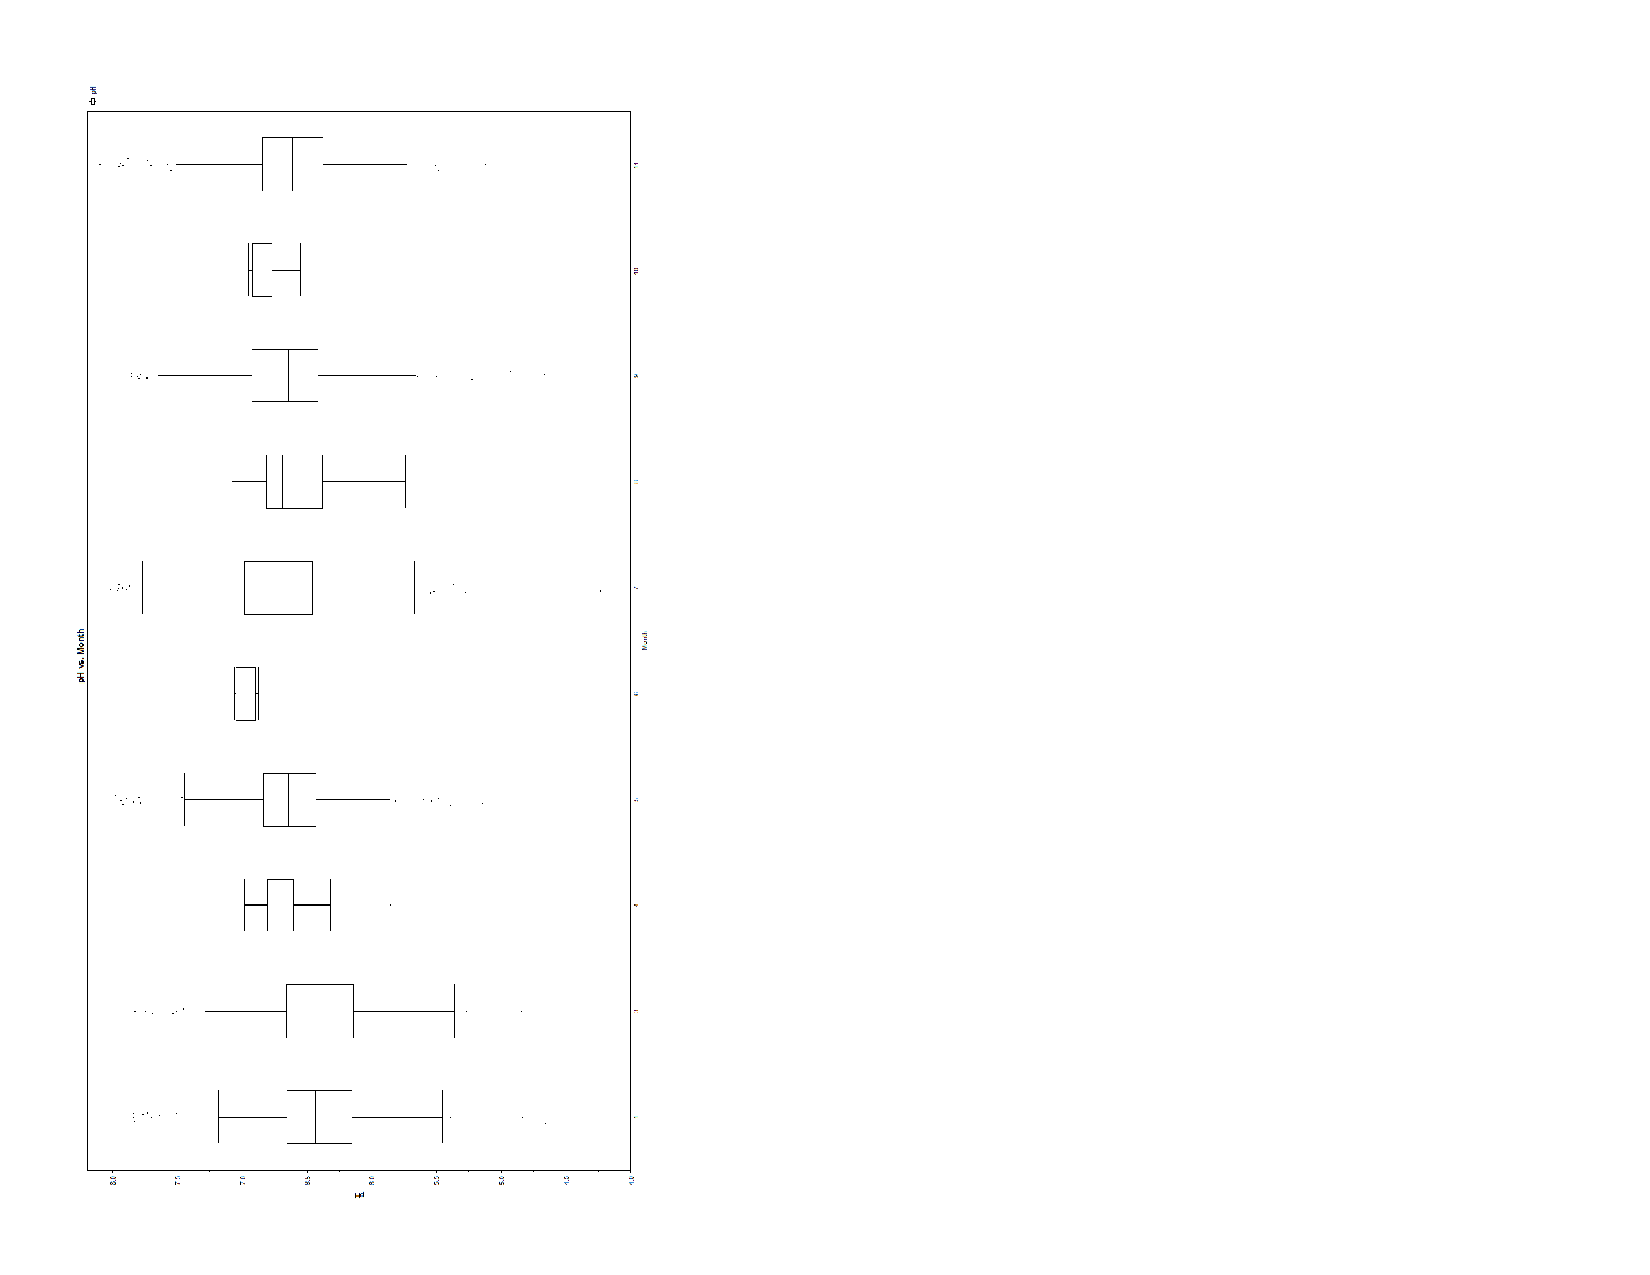
\includepdf[noautoscale,scale=1.45,offset=350 0,pages=-,linktodoc]{figures/CAGraph1}

\phantomsection
\label{CAGraph2}
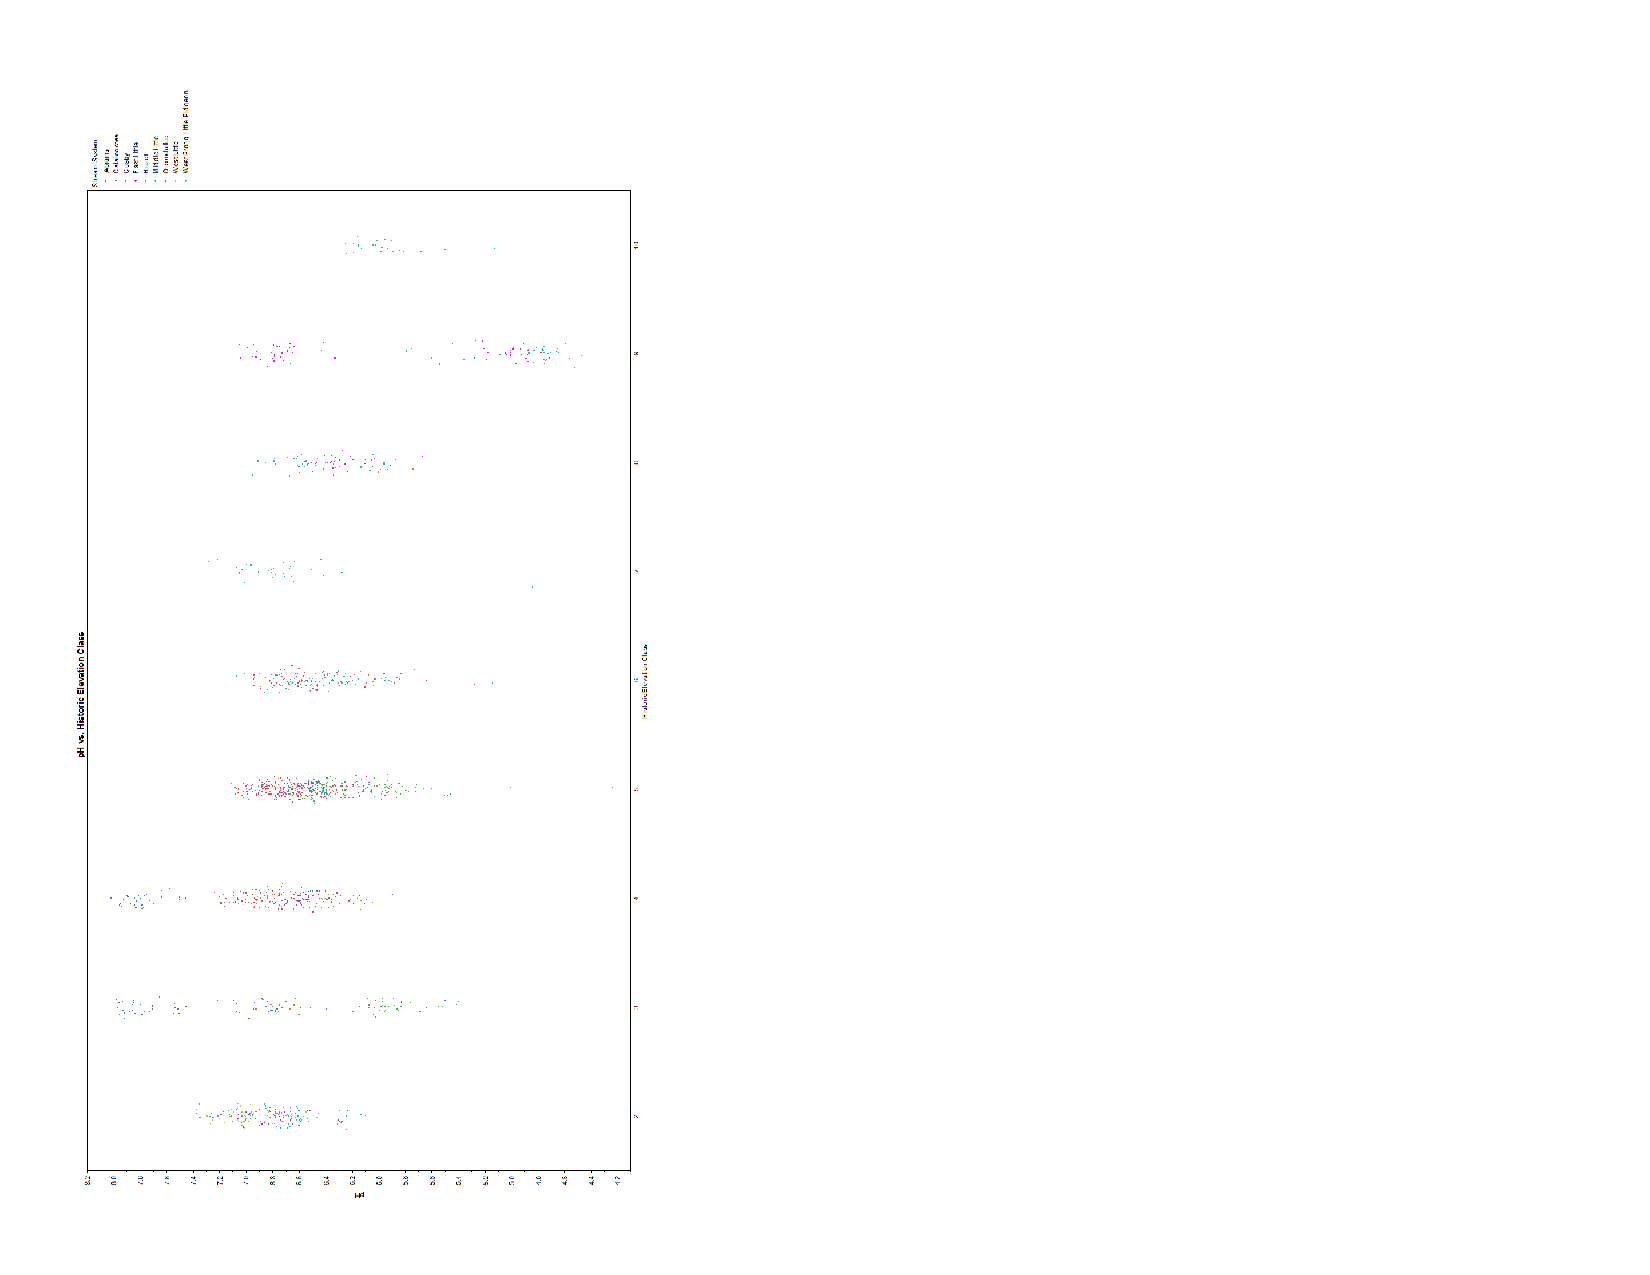
\includepdf[noautoscale,scale=1.45,offset=350 0,pages=-,linktodoc]{figures/CAGraph2}

\phantomsection
\label{CAGraph3}
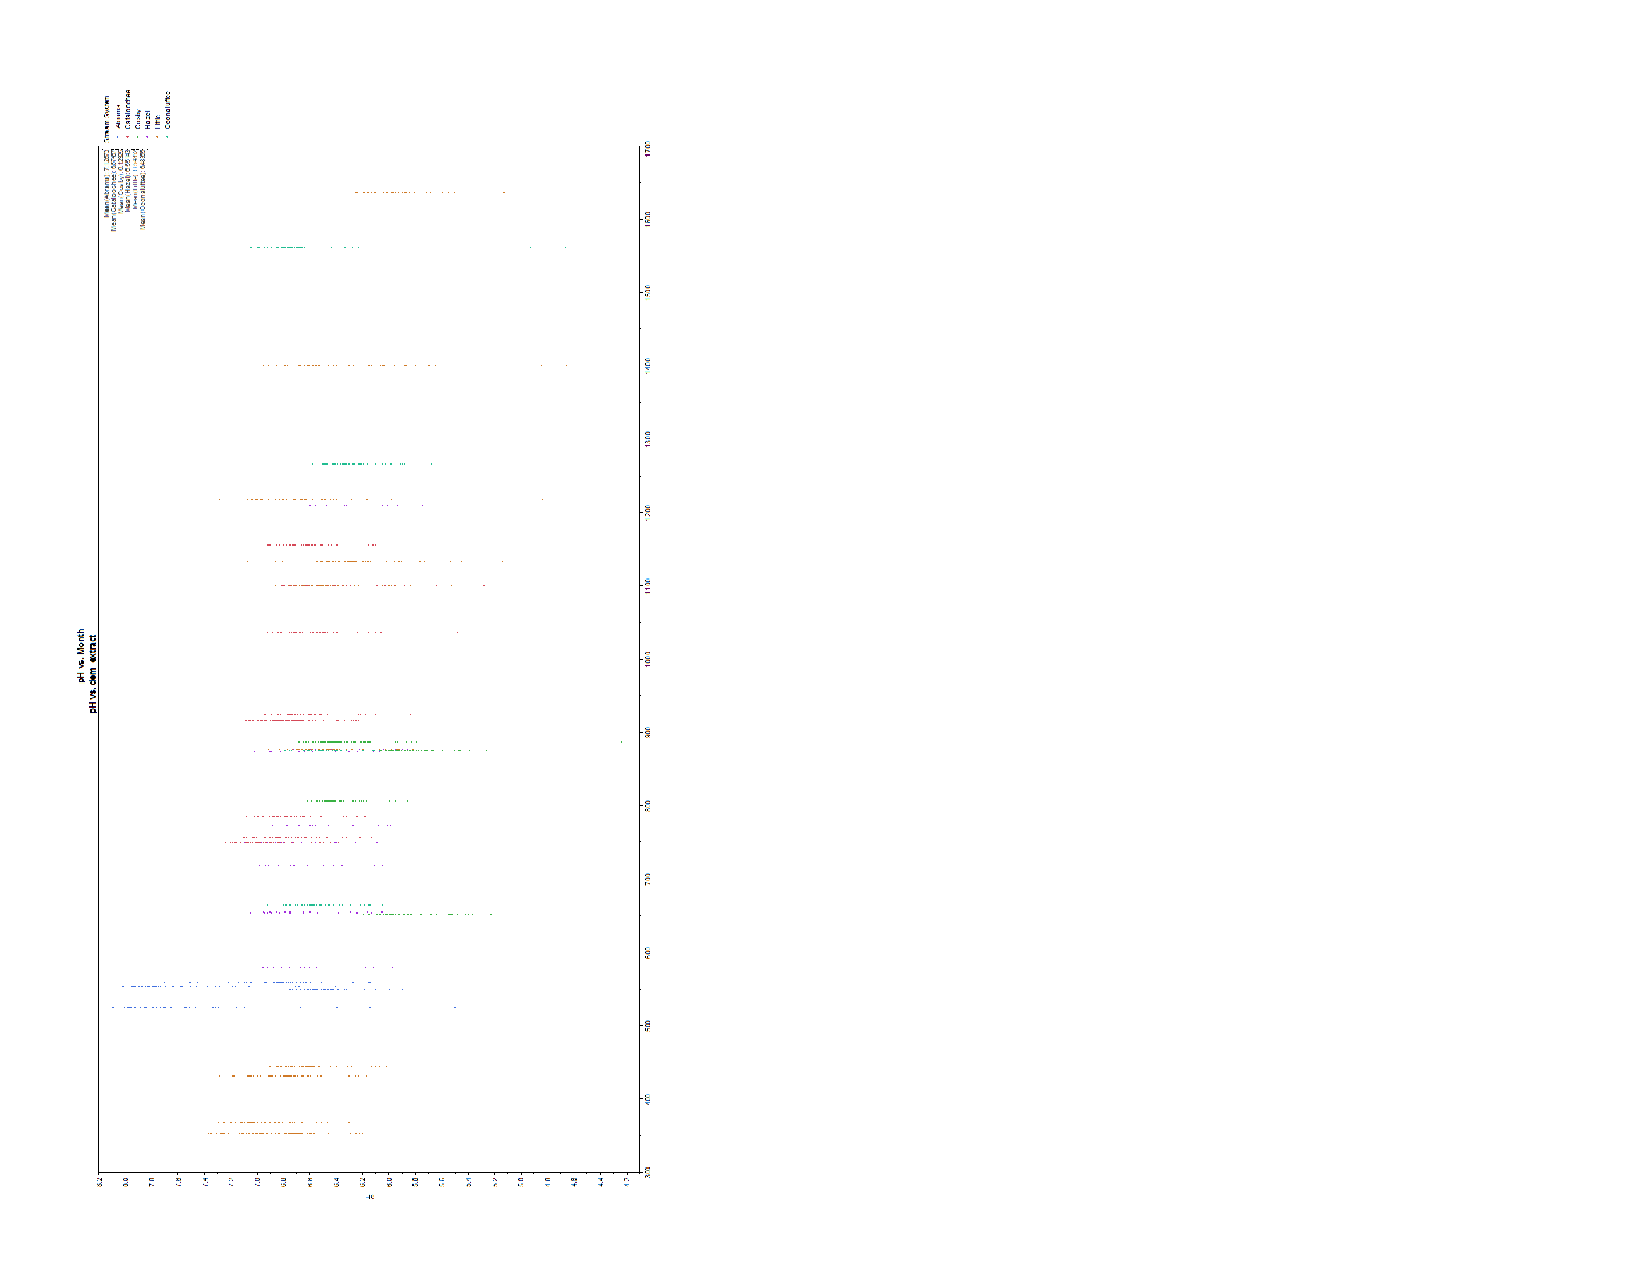
\includepdf[noautoscale,scale=1.45,offset=350 0,pages=-,linktodoc]{figures/CAGraph3}

\phantomsection
\label{CAGraph6}
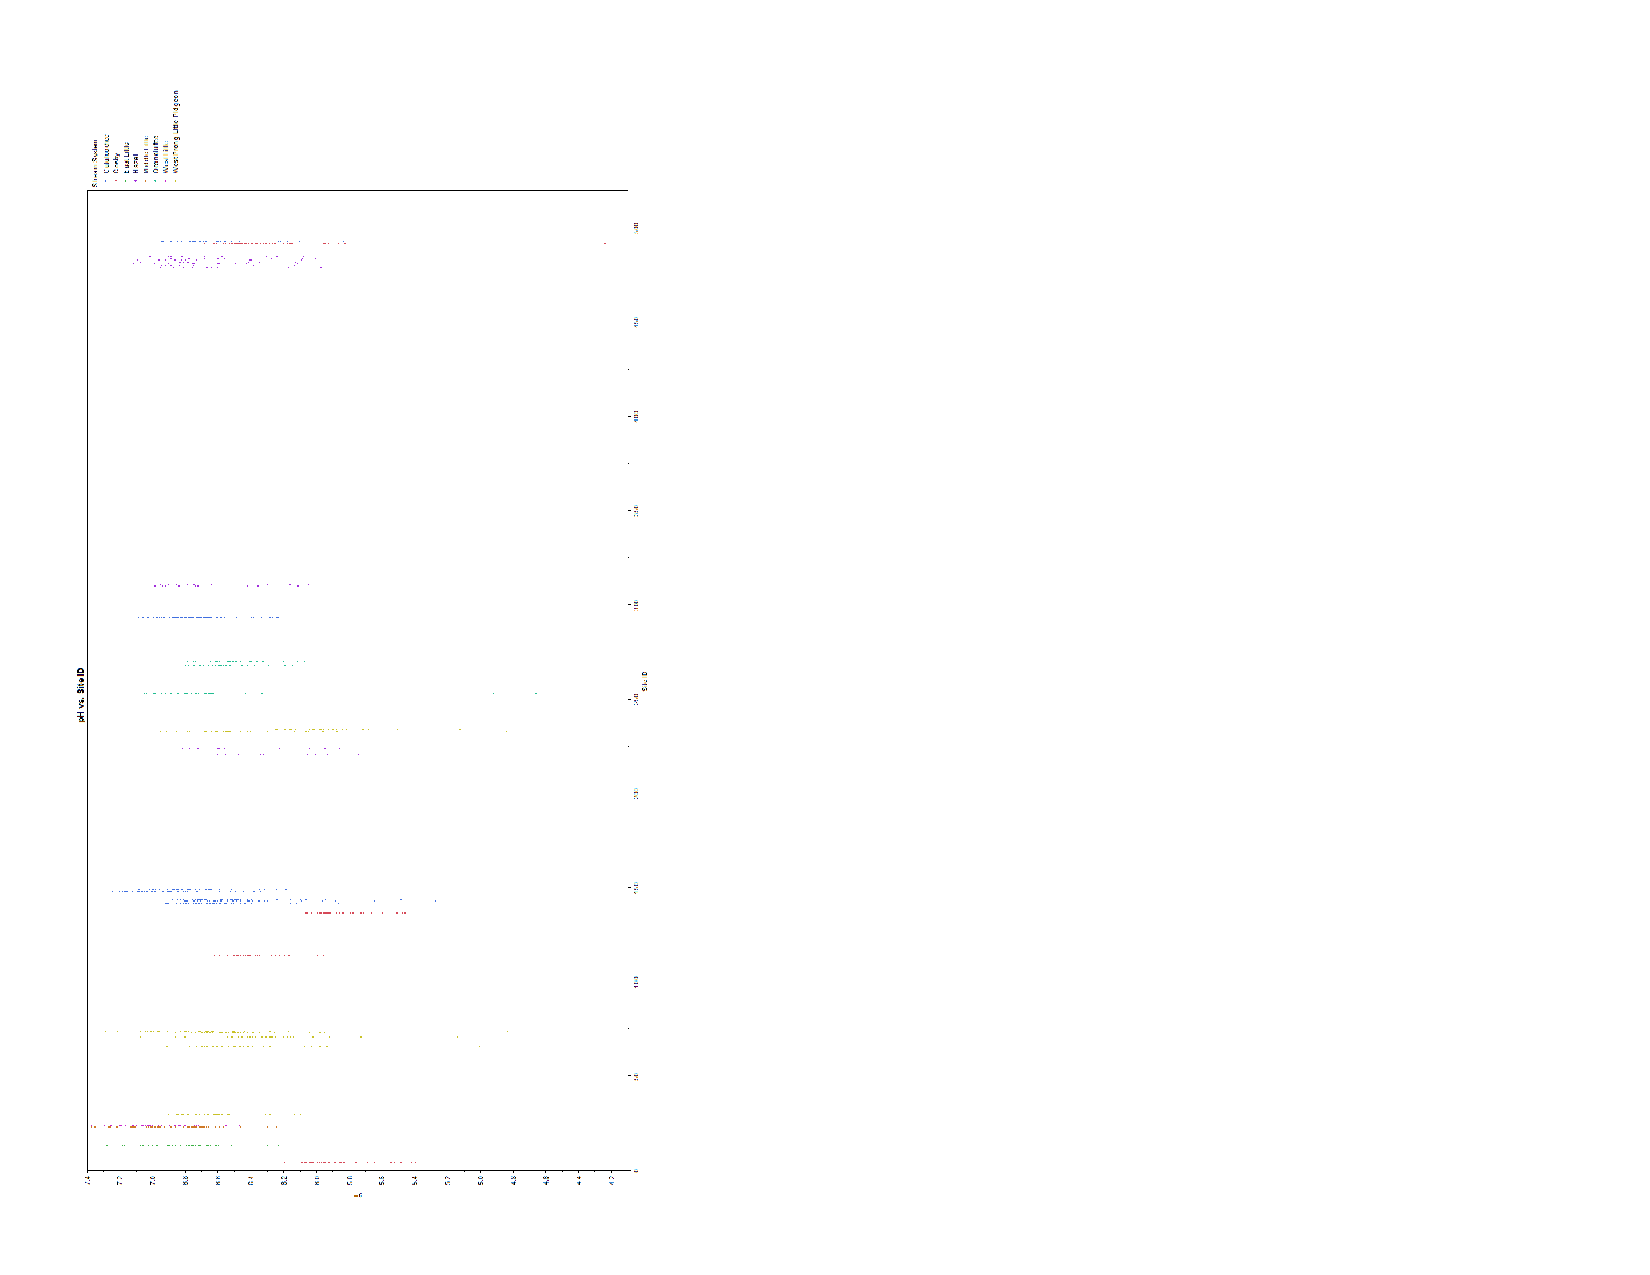
\includepdf[noautoscale,scale=1.45,offset=350 0,pages=-,linktodoc]{figures/CAGraph6}

\phantomsection
\label{CAGraph8}
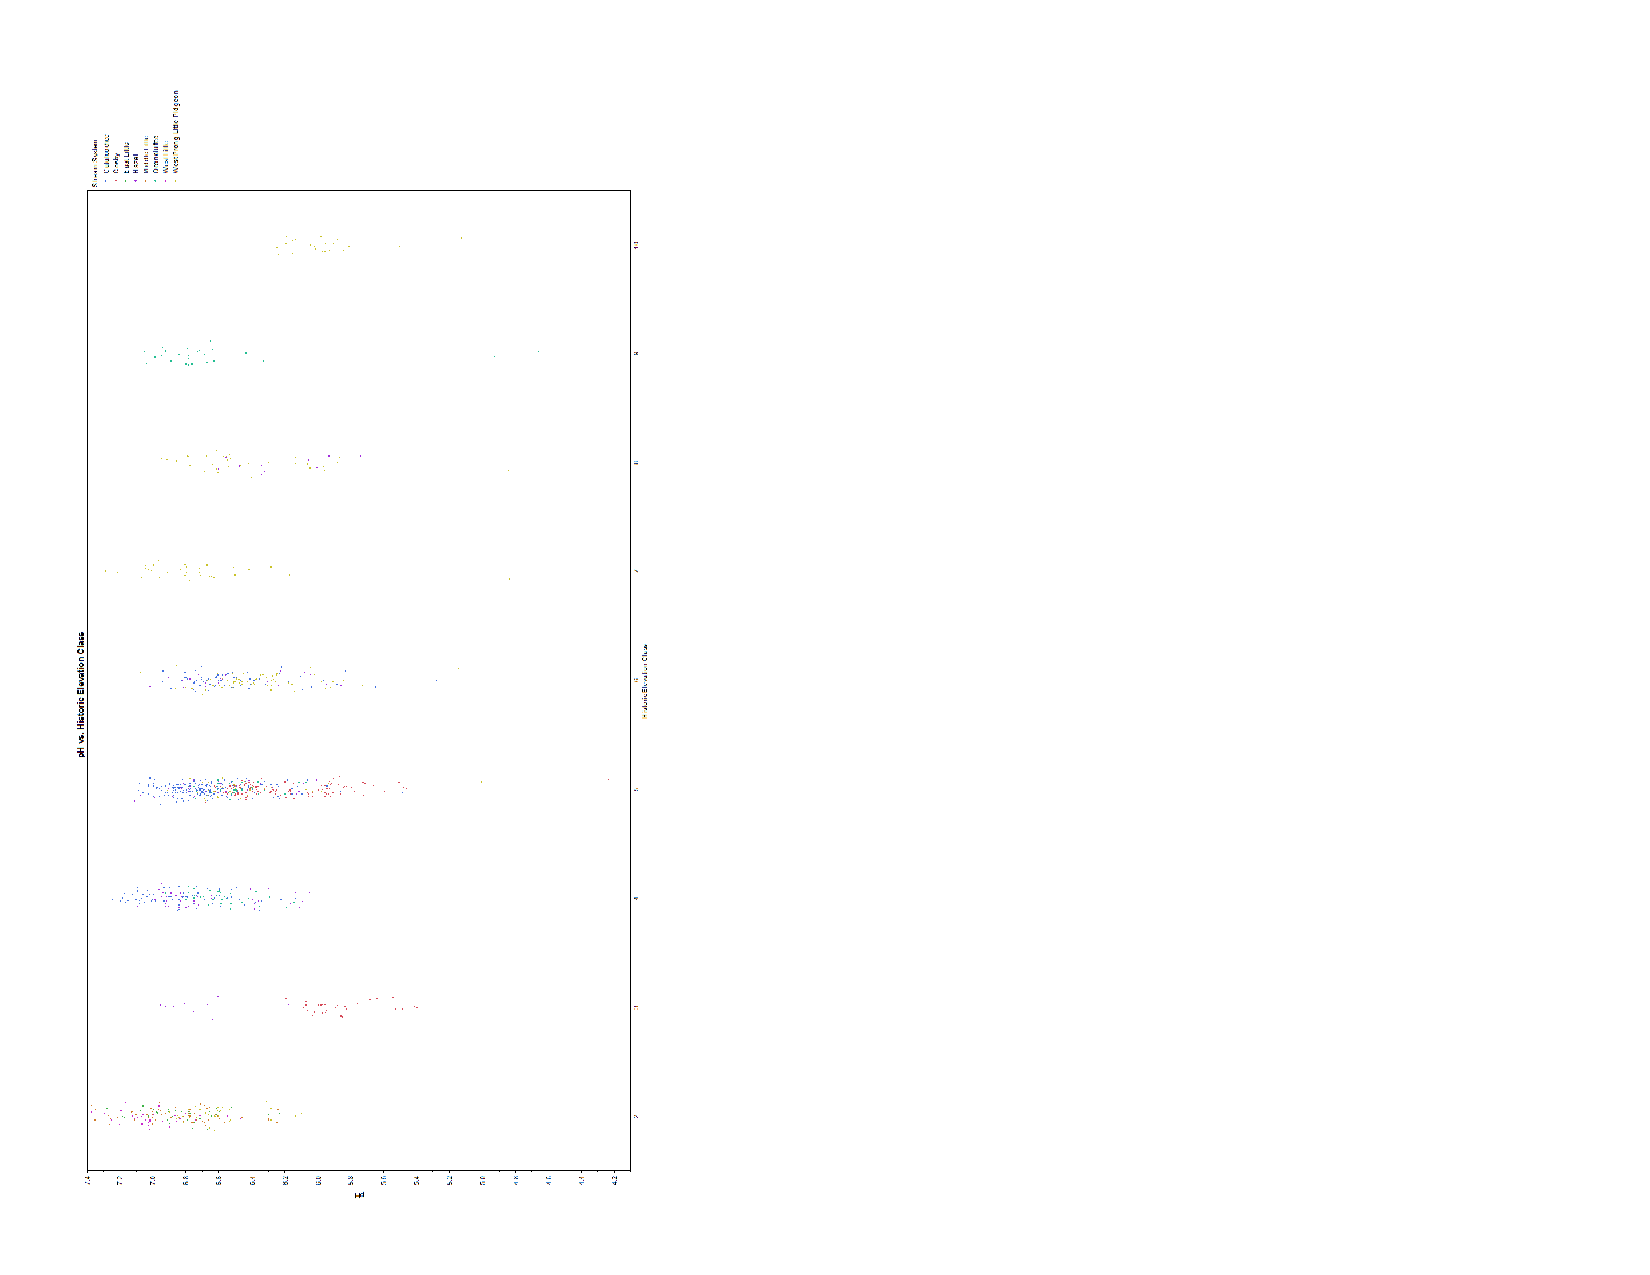
\includepdf[noautoscale,scale=1.45,offset=350 0,pages=-,linktodoc]{figures/CAGraph8}

\phantomsection
\label{CAGraph9}
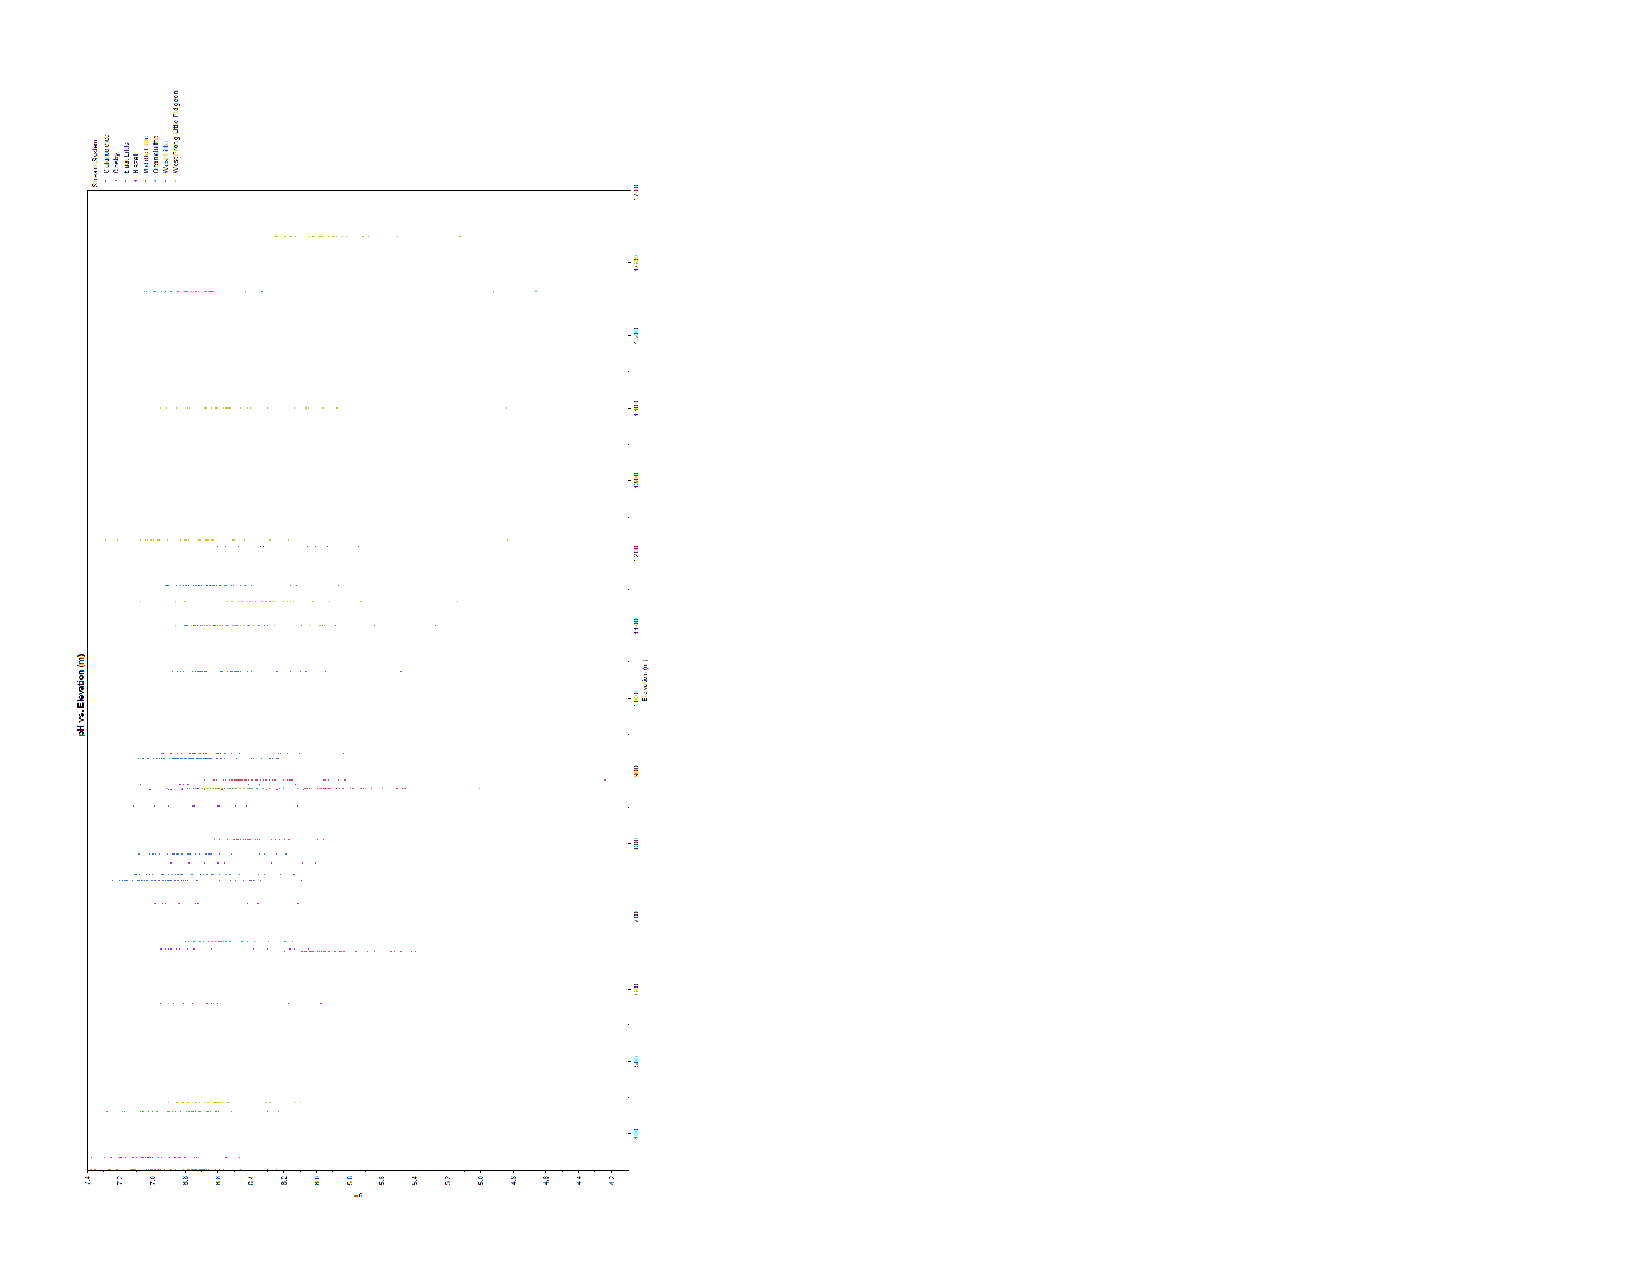
\includepdf[noautoscale,scale=1.45,offset=350 0,pages=-,linktodoc]{figures/CAGraph9}

\phantomsection
\label{CAGraph10}
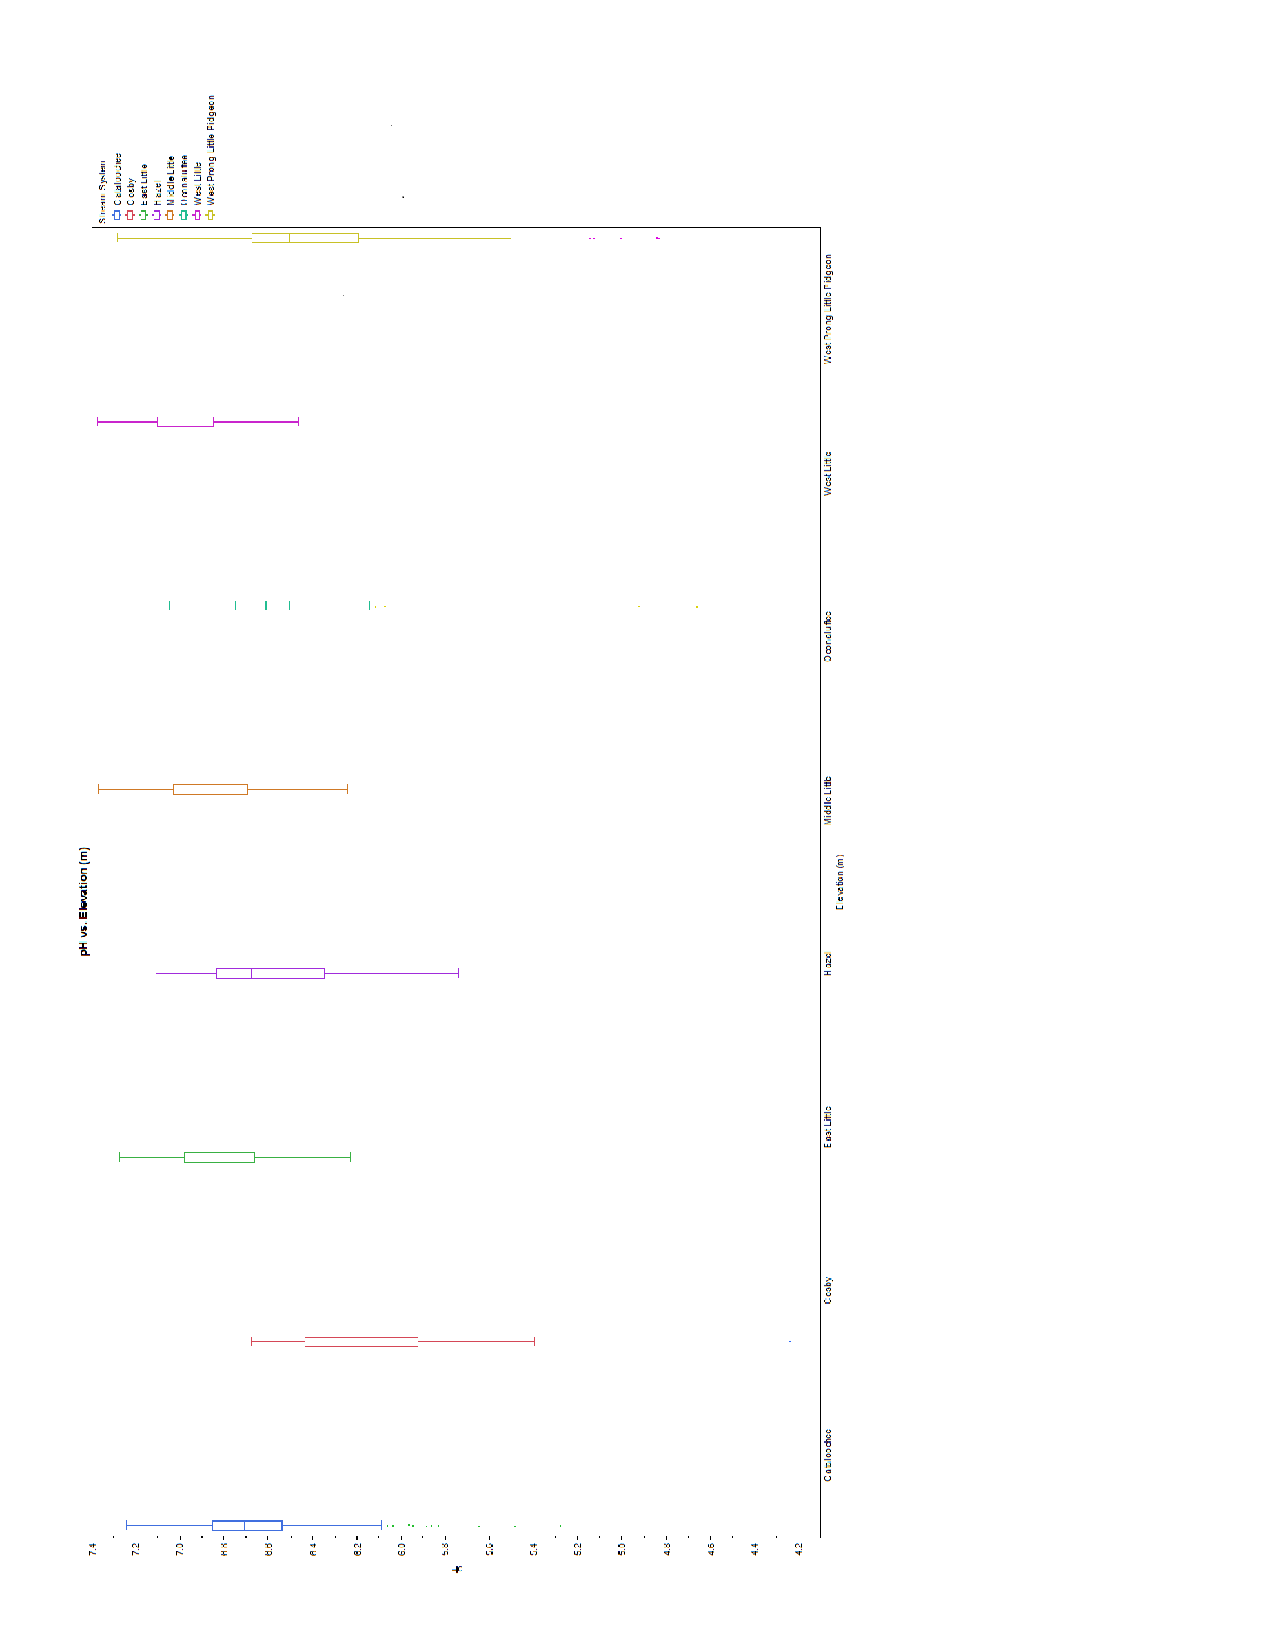
\includepdf[noautoscale,scale=1,offset=100 0,pages=-,linktodoc]{figures/CAGraph10}





















    %%%%%%%%%%%%%%%%%%%%%%%%%%%%%%%%%%%%%%%%%%%%%%%%%%%%%%%%%%%%%%%%%%%%%%%%%%%%%%%%%%%%%%%%%%%%%%%%%%%%%
    % A VITA IS REQUIRED
    %%%%%%%%%%%%%%%%%%%%%%%%%%%%%%%%%%%%%%%%%%%%%%%%%%%%%%%%%%%%%%%%%%%%%%%%%%%%%%%%%%%%%%%%%%%%%%%%%%%%%
    \addToTOC{Vita}
    \chapter*{Vita} \label{ch:vita}
Tim Pobst was born in Nashville, TN on June 1st 1985 to George and Peggy Pobst.  He graduated from Centennial High School near Franklin, TN and was accepted to the University of Tennessee immediately after.  He was undecided for three years before deciding to try for a civil engineering degree and he finished it in spring of 2011.  He stayed at  the University of Tennessee to get a masters degree in environmental engineering under Dr. Schwartz.
\end{document}
